\documentclass[11pt]{article}
\usepackage[T1]{fontenc}
\usepackage{mathpazo}
\renewcommand{\ttdefault}{pcr}
\usepackage{amsmath,amssymb,amsthm,mathtools}
\usepackage[a4paper,margin=27mm]{geometry}
\usepackage{microtype,graphicx,booktabs,array,xcolor}
\usepackage[colorlinks=true,linkcolor=blue!45!black,citecolor=blue!45!black,urlcolor=blue!45!black]{hyperref}
\urlstyle{same}
\setlength{\emergencystretch}{2em}
\pdftrailerid{}
\pdfgentounicode=1
\pdfglyphtounicode{parenleftbig}{0028}
\pdfglyphtounicode{parenrightbig}{0029}
\pdfglyphtounicode{bracketleftbig}{005B}
\pdfglyphtounicode{bracketrightbig}{005D}
\pdfglyphtounicode{braceleftbig}{007B}
\pdfglyphtounicode{bracerightbig}{007D}
\pdfglyphtounicode{vextendsingle}{23D0}
\pdfglyphtounicode{parenleftBig}{0028}
\pdfglyphtounicode{parenrightBig}{0029}
\pdfglyphtounicode{parenleftbigg}{0028}
\pdfglyphtounicode{parenrightbigg}{0029}
\pdfglyphtounicode{bracketleftbigg}{005B}
\pdfglyphtounicode{bracketrightbigg}{005D}
\pdfglyphtounicode{floorleftbigg}{230A}
\pdfglyphtounicode{floorrightbigg}{230B}
\pdfglyphtounicode{ceilingleftbigg}{2308}
\pdfglyphtounicode{ceilingrightbigg}{2309}
\pdfglyphtounicode{braceleftbigg}{007B}
\pdfglyphtounicode{bracerightbigg}{007D}
\pdfglyphtounicode{parenleftBigg}{0028}
\pdfglyphtounicode{parenrightBigg}{0029}
\pdfglyphtounicode{bracketleftBigg}{005B}
\pdfglyphtounicode{bracketrightBigg}{005D}
\pdfglyphtounicode{floorleftBigg}{230A}
\pdfglyphtounicode{floorrightBigg}{230B}
\pdfglyphtounicode{ceilingleftBigg}{2308}
\pdfglyphtounicode{ceilingrightBigg}{2309}
\pdfglyphtounicode{braceleftBigg}{007B}
\pdfglyphtounicode{bracerightBigg}{007D}
\pdfglyphtounicode{parenlefttp}{239B}
\pdfglyphtounicode{parenrighttp}{239E}
\pdfglyphtounicode{bracelefttp}{23A7}
\pdfglyphtounicode{braceleftbt}{23A9}
\pdfglyphtounicode{braceleftmid}{23A8}
\pdfglyphtounicode{braceex}{23AA}
\pdfglyphtounicode{parenleftbt}{239D}
\pdfglyphtounicode{parenrightbt}{23A0}
\pdfglyphtounicode{integraltext}{222B}
\pdfglyphtounicode{integraldisplay}{222B}
\pdfglyphtounicode{uniondisplay}{22C3}
\pdfglyphtounicode{intersectiondisplay}{22C2}
\pdfglyphtounicode{hatwide}{0302}
\pdfglyphtounicode{tildewide}{0303}
\pdfglyphtounicode{radicalbig}{221A}
\pdfglyphtounicode{mapsto}{007C} %

\numberwithin{equation}{section}
\newtheorem{theorem}{Theorem}[section]
\newtheorem{proposition}[theorem]{Proposition}
\newtheorem{lemma}[theorem]{Lemma}
\newtheorem{corollary}[theorem]{Corollary}
\theoremstyle{definition}
\newtheorem{definition}[theorem]{Definition}
\newtheorem{remark}[theorem]{Remark}
\newcommand{\R}{\mathbb R}
\newcommand{\N}{\mathbb N}
\newcommand{\Z}{\mathbb Z}
\newcommand{\E}{\mathbb E}
\newcommand{\one}{\mathbf 1}
\DeclareMathOperator{\OPT}{OPT}
\DeclareMathOperator{\cost}{cost}
\DeclareMathOperator{\diam}{diam}
\DeclareMathOperator{\supp}{supp}
\DeclareMathOperator{\Lip}{Lip}
\DeclareMathOperator{\dist}{dist}
\DeclareMathOperator*{\argmin}{arg\,min}

\title{Squared-logarithmic randomized \(k\)-server\\
on arbitrary metrics}
\hypersetup{pdftitle={Squared-logarithmic randomized k-server on arbitrary metrics},pdfauthor={OpenAI}}
\author{OpenAI}
\date{September 24, 2026}
\begin{document}
\maketitle
\begin{abstract}
We prove that randomized \(k\)-server has competitive ratio
\(O((\log(k+1))^2)\) on every metric space against oblivious request
sequences, matching the known worst-case lower bound. For each metric
and initial configuration, one policy works for all finite request
sequences, including on infinite and unbounded spaces. When the initial
server positions are distinct, no additive term is needed.
\end{abstract}
\tableofcontents
\section{Introduction}\label{sec:introduction}

The \(k\)-server problem asks how to move \(k\) servers in a metric
space when requests arrive one at a time. A request is a point that
must be occupied by a server; the cost is the distance moved.
The offline optimum knows all future requests, whereas an online
policy must decide from the revealed prefix. We determine the sharp
worst-case order of the randomized competitive ratio.

More precisely, let \((X,d)\) be a metric space and let
\(s=(s_1,\ldots,s_k)\in X^k\) be the initial positions of \(k\)
labeled servers. Repeated positions are allowed. To serve \(r_t\),
a policy chooses one server and moves it to \(r_t\), leaving all
others fixed. A server already at \(r_t\) can be chosen at zero cost.
For a finite request sequence \(\sigma\), let
\(\cost_{A,s}(\sigma)\) be a policy's total movement and let
\(\OPT_{X,d,k,s}(\sigma)\) be the minimum such cost with full
knowledge of \(\sigma\). Requests are fixed independently of the
policy's random choices, the usual oblivious-adversary model.

\begin{theorem}\label{thm:main}
There is an absolute constant \(C<\infty\) such that, for every
integer \(k\ge2\), every metric space \((X,d)\) with at least \(k+1\)
points, and every \(s\in X^k\), there exist a randomized online policy
\(A\) and a finite \(B\ge0\) satisfying
\begin{equation}\label{eq:main}
 \E\,\cost_{A,s}(\sigma)
 \le C\bigl(\log(k+1)\bigr)^2\OPT_{X,d,k,s}(\sigma)+B
\end{equation}
for every finite request sequence \(\sigma\).
The constant \(C\) is independent of every property of the metric.
The number \(B\) may depend on \((X,d),k,s\), but not on the sequence
or its length. The same policy serves all finite sequences and
horizons. If the initial positions are distinct, one may take \(B=0\).
\end{theorem}

There is no finiteness, boundedness, or discreteness assumption on
\(X\), and no computational-efficiency claim for the policy.
Throughout, logarithms are natural.

\subsection{Context and previous work}

Manasse, McGeoch, and Sleator introduced the \(k\)-server problem as a
common framework for online service problems
\cite{MMS88,MMS90}. They proved the deterministic lower bound \(k\)
on every metric with more than \(k\) points and conjectured that it is
attainable. Koutsoupias and Papadimitriou established the
\((2k-1)\)-competitive work function algorithm \cite{KP95}.
A recent preprint of Coester, Koutsoupias, and Zbysiński announces a
\(k\)-competitive analysis of that algorithm \cite{CKZ26}.
The present paper concerns the different asymptotic behavior made
possible by randomization against oblivious requests.

Paging, the case of a uniform metric, gave the basic reason to expect
such an improvement. Fiat, Karp, Luby, McGeoch, Sleator, and Young
proved a harmonic lower bound and a \(2H_k\)-competitive randomized
marking algorithm \cite{FKLMSY91}; McGeoch and Sleator attained the
exact bound \(H_k=\sum_{i=1}^k i^{-1}\) \cite{MS91}.
For weighted paging, Bansal, Buchbinder, and Naor obtained the optimal
order \(O(\log k)\) through a fractional primal-dual algorithm and
online rounding \cite{BBN12}. These results formed part of the
evidence for the folklore randomized \(k\)-server conjecture, which
predicted \(O(\log k)\) on every metric.

That conjecture was disproved by Bubeck, Coester, and Rabani
\cite[Theorem~11 and Proposition~8]{BCR23}: there exist
\((k+1)\)-point metrics requiring
competitive ratio \(\Omega(\log^2 k)\), even allowing a fixed additive
constant. Their result must be distinguished from a lower bound
on every metric. The latter developed through the decomposition and
metric Ramsey methods of Karloff, Rabani, and Ravid \cite{KRR94},
Blum, Karloff, Rabani, and Saks \cite{BKRS00}, Bartal, Bollobás,
and Mendel \cite{BBM06}, and Bartal, Linial, Mendel, and Naor
\cite{BLMN05}; Bubeck, Coester, and Rabani ultimately obtained the
sharp universal order \(\Omega(\log k)\)
\cite[Corollary~20]{BCR23}.
Theorem~\ref{thm:main} matches the larger, worst-case lower bound.
It establishes the sharp squared-logarithmic order after the negative
resolution of the original logarithmic conjecture.

The main upper-bound approach passes through hierarchically separated
trees. Bartal introduced probabilistic approximation by these
metrics \cite{Bartal96,Bartal98}, and Fakcharoenphol, Rao, and Talwar
obtained expected distortion \(O(\log n)\) for \(n\)-point metrics
\cite{FRT04}. Recursive allocation methods were developed by
Coté, Meyerson, and Poplawski \cite{CMP08} and by Bansal, Buchbinder,
and Naor \cite{BBN10}. Bansal, Buchbinder, Mądry, and Naor then gave
the first polylogarithmic bound for arbitrary finite metrics,
\(O(\log^2 k\,\log^3 n\,\log\log n)\) \cite{BBMN15}.
Bubeck, Cohen, Lee, Lee, and Mądry achieved \(O(\log^2 k)\) on HSTs
using multiscale entropic regularization \cite{BCLLM18}.
The static embedding reduction yields \(O(\log^2 k\log n)\) on
general finite metrics. Its dependence on \(n\) does not give a
bound in \(k\) alone.
Coester and Cosson recently made the HST and finite-metric bounds
polynomial-time, using a total number of random bits independent of the
request length \cite[Theorem~1 and Corollary~2]{CoesterCosson2026}.
Their general finite-metric ratio retains the factor $\log n$.

Changing the embedding as requests arrive is also an established
direction. The dynamic construction of \cite[Section~4]{BCLLM18}
gives \(O(\log^3 k\log(1+\Delta))\) on finite metrics, where
\(\Delta\) is the ratio
of the largest distance to the smallest positive distance.
Lee's evolving, fusible HST framework used heavy-ball nets to merge
clusters near concentrated mass and introduced a fission potential intended
to pay for later splits \cite[Sections~3.1.2--3.2 and~5.3]{Lee18}.
Its general competitive-ratio claim was withdrawn after a gap in
Section~5.3.2 \cite{LeeErratum}. Heavy-ball protection and accounting
for changing partitions are methodological antecedents of our
construction. Here the partition schedule is driven by the posterior
measure of a hidden comparator; it produces a fixed tree of label
strings. We prove the required edit and retained-anchor travel estimates
in Sections~\ref{sec:partitions} and~\ref{sec:travel}, without invoking
a theorem from the withdrawn argument.

Subtree-rank coordinates, internal supermeasures, and
fractional-to-integral transfer already play central roles in
\cite{BBMN15,BCLLM18}. The use of local ball-mass ratios and their
telescoping across scales has a geometric predecessor in measured
descent \cite[Lemma~1.7 and Section~1.3]{KLMN05}.
The distributional estimates are converted into a single policy
by finite minimax and product compactness.


\subsection{Main ingredients}

We first establish a finite distributional bound. Given a known law
of requests, select one offline optimum for each input and use only
its posterior distributions conditional on the revealed prefix.
This does not reveal the realized future.

The construction starts with partitions of the finite metric at several
distance scales. A point's complete tuple of cell labels identifies a
leaf of a fixed tree. The hidden optimum then gives posterior distributions
of the server counts below each tree vertex. We use those distributions to allocate
fractional server mass on the tree, represent that mass by points of
the original metric, and round it to exactly $k$ servers. Changes of
the partitions and of the representatives must be charged along with
movement of mass through the tree. One logarithm comes from the
partition estimate and one from the allocation estimate; rounding
and realization preserve their product.

For exposition we prove the reusable allocation theorem first, then
construct its partition input. The four components are as follows.

\paragraph{Allocation from subtree count distributions.}
On a fixed separated tree, we maintain fractional subtree amounts
with movement \(O(\log(k+1))\) times that of the hidden comparator.
The amounts dominate the serving requirement and are bounded above
by a constant multiple of the posterior expected counts. They may
park at internal vertices, keeping unused mass above children while
their posterior proportions change. The proof uses convex rank functions
and slowly varying proportions. A separate rule for a nearly dominant
child chooses the allocations to the other children first and gives that child
the remaining parent amount, subject to its cap. This fits all children
within their rank bounds without an additional logarithm.
The resulting allocation theorem applies
to general observed hidden trajectories, independently of the later
metric embedding.

\paragraph{A compact variational potential.}
The partition analysis uses a finite-dimensional minimum over
separated auxiliary sites with positive-part capacity constraints.
Concentration forces a nearly full site near the request.
A feasible relocation of that site makes the optimal integrand
have small positive slope there. Ball-mass ratios and inner
moments then telescope over scales, giving a single logarithm in
the measure-motion budget. All geometric radii in this argument
are fixed numerical multiples of the scale.

\paragraph{Partitions adapted to local mass ratios.}
Heavy balls protect highly concentrated requests. Other requests
use chronological rosters in doubling qualification tiers.
Their first-hit loss depends on a local mass ratio rather than on
one worst-case logarithm at every level. Random retirements keep
the rosters bounded; a separate short-lived auxiliary roster pays
the retirement errors. The resulting finite label sets are fixed
independently of the request horizon.

\paragraph{Moving representatives and rounding.}
Fractional mass parked at a tree vertex is represented by an anchor
in the original metric. Retained anchors can move even when no mass
crosses a tree edge. A normalized affine potential and a pointwise
sum of parked-mass coefficients pay this travel without multiplying
the tree movement by another logarithm. A dynamic balanced-rounding
lemma, allowing correlated parent and child states, incurs only an
absolute loss.

These components give two logarithms in total. The final step removes
the finite-metric additive term by independent episodes and reset
blocks, then uses finite-dimensional separation and compactness.
This yields a single policy on all finite inputs of an arbitrary
metric, including unbounded spaces. A matching simulation handles
repeated initial positions.

\subsection{Organization}

Section~\ref{sec:setup} fixes the probabilistic conventions and the
movement accounting. Sections~\ref{sec:allocation},
\ref{sec:proportions}, and~\ref{sec:allocation-finish} prove the
tree allocation theorem. Section~\ref{sec:pilot} develops the
variational potential, and Section~\ref{sec:partitions} constructs
the changing partitions. Sections~\ref{sec:travel}
and~\ref{sec:rounding} control realization and rounding.
Section~\ref{sec:transfer} proves the uniform-policy conclusion.

The geometric and algorithmic estimates are proved below.
The final passage to arbitrary spaces uses the standard compactness
theorem identified in Section~\ref{sec:transfer}; the worst-case lower
bound is the result of Bubeck, Coester, and Rabani cited above.

\section{Finite laws, posterior motion, and the proof architecture}\label{sec:setup}

We first allow the policy to know a finite input law. This permits
conditional distributions of an offline optimum, while still forbidding
the policy from observing the realized future. The estimate obtained in
this setting must have an additive term uniform in the law and horizon.
Section~\ref{sec:transfer} uses precisely this uniformity to construct
one policy on an arbitrary metric.

\subsection{Matching and lazy simulation}

A configuration is a multiset of \(k\) points, with each repeated
point counted separately. For two configurations \(A=(a_1,\ldots,a_k)\)
and \(C=(c_1,\ldots,c_k)\), put
\[
 \mathsf M(A,C)=\min_{\pi\in S_k}\sum_{i=1}^k d(a_i,c_{\pi(i)}).
\]
This distance ignores the labels when matching configurations; an
actual server retains its label when it moves. A \emph{simulated}
configuration may move several members between requests. Its movement
cost is the matching distance between its successive configurations.
A policy is \emph{strongly lazy} if it does nothing when a server already
occupies the request, and otherwise moves exactly one server to it.

The classical cost-nonincreasing lazy reduction for the same starting
configuration is due to Manasse, McGeoch, and Sleator
\cite[Lemma~1, p.~211]{MMS90}. The matching-potential formulation below
also permits an arbitrary initial mismatch.

\begin{lemma}[Lazy simulation]\label{lem:lazy-simulation}
Suppose a causal sequence of simulated configurations
\(C_0,C_1,\ldots,C_H\) contains the request \(r_t\) at each time
\(t\ge1\). From any actual start \(A_0\), a strongly lazy policy serves
the same requests and satisfies, pathwise,
\[
 \cost(A_0;r_1,\ldots,r_H)
 \le \mathsf M(A_0,C_0)+\sum_{t=1}^H\mathsf M(C_{t-1},C_t).
\]
The conclusion also holds if the matching distances on the right are
replaced by any larger specified movement costs.
\end{lemma}

\begin{proof}
After \(C_t\) is revealed, take a minimum matching from \(A_{t-1}\)
to \(C_t\). If \(A_{t-1}\) does not contain \(r_t\), move the actual
server matched to a chosen occurrence of \(r_t\) in \(C_t\) to that
point. Keeping the same matching after the move shows that
\[
 \text{actual cost at }t+\mathsf M(A_t,C_t)
 \le \mathsf M(A_{t-1},C_t).
\]
If the request was already covered, make no move and the inequality
holds with equality. Composing minimum matchings gives
\[
 \mathsf M(A_{t-1},C_t)
 \le \mathsf M(A_{t-1},C_{t-1})
       +\mathsf M(C_{t-1},C_t).
\]
Summing and discarding the nonnegative final matching distance proves
the claim. Minimum matchings exist because there are only \(k!\)
permutations, even with repeated positions. Fixed orders resolve all
ties, so this procedure is causal.
\end{proof}

The same pathwise inequality applies to any prescribed simulated
trajectory. Causality is needed to obtain an online policy from it;
when comparing two offline optima, only the pathwise inequality is
used.

We use the shorthand
\[
                         \ell=1+\log(k+1).
\]
All unnamed multiplicative constants below are absolute. Constants may
depend on numerical parameters only after those parameters have been
fixed once and for all, independently of \(k\) and the metric.

\begin{proposition}[Finite distributional estimate]\label{prop:finite-law}
There is an absolute \(a<\infty\) with the following property. For every
finite metric \(Y\) of positive diameter, every \(k\ge2\), and every
start \(s\in Y^k\), there is a finite \(D_0=D_0(Y,k,s)\) such that,
for every finite horizon \(H\) and every probability law on \(Y^H\),
there is a causal strongly lazy policy satisfying
\begin{equation}\label{eq:finite-law}
             \E\,\cost\le a\ell^2\E\,\OPT+D_0 .
\end{equation}
The policy may depend on the law and horizon. The number \(D_0\)
does not.
\end{proposition}

Sections~\ref{sec:allocation}--\ref{sec:rounding} prove this
proposition. An additive term in those sections is always bounded by
a fixed finite function of \(Y,k,s\) and the finite structures
constructed from them. It never depends on the law, horizon, number
of histories, or number of updates. We will verify this distinction
again when assembling the estimates.

\subsection{Hidden comparators and the two parts of a posterior update}

Fix the data of Proposition~\ref{prop:finite-law}. For each input,
choose one optimum trajectory of the \(k\) labeled servers, resolving
ties by a fixed order. Such a choice exists: each request has only
\(k\) possible server labels, so a length-\(H\) input has only \(k^H\)
candidate trajectories. The chosen optimum is a hidden random variable
determined by the input. Set
\[
                         Q=\E\,\OPT .
\]
The policy uses conditional laws of this trajectory, not its hidden
realization.

Let \(\mathcal F_t\) contain the request prefix through time \(t\)
and the independent random tape used to construct the partitions.
It is convenient to include that entire tape from time zero. The
rounding procedure will use a separate independent tape that is
excluded from \(\mathcal F_t\). Thus conditioning on \(\mathcal F_t\)
does not alter the true-metric comparator posterior beyond
conditioning on the request prefix.

For any old hidden quantity \(Z_{t-1}\), a step has two logically
different parts:
\[
 \mathcal L(Z_{t-1}\mid\mathcal F_{t-1})
 \xrightarrow{\mathrm{filtering}}
 \mathcal L(Z_{t-1}\mid\mathcal F_t)
 \xrightarrow{\mathrm{drift}}
 \mathcal L(Z_t\mid\mathcal F_t).
\]
Here \(\mathcal L\) denotes a probability law, not the pilot potential
introduced later. During filtering, an affine functional with
coefficients held from time \(t-1\) has zero conditional expected
change. A concave functional has nonpositive conditional expected
change. During drift, the joint conditional law of
\((Z_{t-1},Z_t)\) provides a coupling. For embedded quantities, the
old variable uses the old map and the new variable uses the new map.

All signed filtering estimates are applied over every step, with old
parameters held fixed, \emph{before} selecting resets or partition
edits. In particular, no argument conditions a martingale estimate on
the later event that a reset is necessary.

For probability estimates concerning random radii or retirements, we
use a different conditioning: fix the true input and its comparator
trajectory, and average over the partition tape. The relevant
insertion schedules will then be deterministic. This does not assert
independence after conditioning on the entire tape in \(\mathcal F_t\).

At a fixed finite horizon all relevant random outcomes can be taken
finite. A radius draw need only specify which subset of the finite
space is its ball; a roster lifetime has a finite maximum age.
Only finitely many insertions can occur. More explicitly, preallocate
at most \(H\) insertion slots per level and structure, discretize each radius
at all pairwise distances in \(Y\), and preallocate each entry's
truncated lifetime. This gives a finite-valued relevant tape, even
before the centers of the inserted balls are known. Any unused
portion of an ambient infinite tape is independent and can be ignored;
all fractional states and selected rounding kernels below depend only
on this finite projection and the request prefix. Realizing a kernel
also uses the current rounded state and the independent rounding
randomness. Conditional laws, minimizing choices, and randomized rounding
kernels can therefore be specified
history by history. Arbitrary continuations are assigned to
zero-probability histories.

\subsection{The true-metric measure update}

Write \(x=r_t\), and designate the server moved by the chosen optimum
at this request, including when its movement is zero. Let
\(\mu^{\mathrm{old}}\) be the expected comparator counting measure
at time \(t-1\), conditional on \(\mathcal F_{t-1}\). At the new
conditioning \(\mathcal F_t\), let \(\mu^-\) and \(\mu^+\) be its
counting measures before and after the move, and let \(\nu\) be the
probability law of the designated mover's old position. Then
\begin{equation}\label{eq:measure-update}
 \mu^+=\mu^--\nu+\delta_x,\qquad
 \nu\le\mu^-,\qquad \nu(Y)=1,\qquad
 e_x=\int_Y d(x,y)\,d\nu(y).
\end{equation}
Both counting measures have total mass \(k\), the measure \(\mu^+\)
has at least one unit at \(x\), and
\[
 \E[\mu^-\mid\mathcal F_{t-1}]=\mu^{\mathrm{old}},
 \qquad
 \E\sum_{t=1}^H e_{r_t}=Q.
\]
The expected counting measure of the stationary members is
\(\mu^+-\delta_x=\mu^--\nu\), hence is bounded by \(\mu^+\).
The separate treatment of this stationary measure and the designated
mover will matter in the partition accounting.

\subsection{Scales and a logarithmic telescope}

Balls are closed. Set \(r_0=\diam Y\) and
\[
 r_j=r_0\tau^{-j},\quad 1\le j\le J,\qquad
       40r_J<\min_{p\ne q}d(p,q).
\]
The separation factor \(\tau\ge2\) is a sufficiently large absolute
constant. Its required lower bounds come from tree allocation and
rounding; neither bound depends on \(k,Y,J\). Once it is fixed,
\(J\) depends only on \(Y\).

\begin{lemma}[Ball-mass telescope]\label{lem:scale-logarithms}
Fix \(0<a<b\), a nonnegative measure \(\mu\), and an offset \(c_0\ge0\).
On a consecutive finite interval of scale indices suppose
\[
 c\le A_j:=c_0+\mu(B(x,ar_j))
 \le B_j:=c_0+\mu(B(x,br_j))\le K,
 \qquad c>0.
\]
If \(p\ge1\) is an integer with \(\tau^p a\ge b\), then
\[
                  \sum_j\log(B_j/A_j)\le p\log(K/c).
\]
\end{lemma}

\begin{proof}
Extend \(A_j\) before the coarsest index of the interval by the value
\(K\). Ball inclusion gives \(B_j\le A_{j-p}\) whenever the shifted
index remains in the interval, and the same inequality follows from
\(B_j\le K\) at the coarse boundary. Thus the sum is at most
\(\sum_j(\log A_{j-p}-\log A_j)\). All interior terms cancel, leaving
at most \(p\) coarse-end terms minus at most \(p\) fine-end terms.
Each resulting difference is at most \(\log(K/c)\).
\end{proof}

In every application, \(a,b,c\) are fixed positive constants and
\(K=O(k+1)\), so the bound is \(O(\ell)\). The offset permits its use
with \(1+\mu(B)\) as well as with positive ball masses themselves.
Geometric sums of radii, by contrast, cost an absolute multiple of
their largest radius and introduce no logarithm.

\subsection{Where the two logarithms occur}

The allocation theorem begins with a fixed finite tree and a hidden
trajectory of \(k\) members on its leaves. It constructs subtree
amounts \(q_v\) satisfying
\[
 q_{\mathrm{root}}=k,\qquad
 \sum_{i\text{ child of }v}q_i\le q_v,\qquad
                    q_v\le C_0m_v,
\]
where \(m_v\) is the posterior expected hidden subtree count.
The inequality in conservation allows \emph{parking} at internal
vertices:
\[
                  p_v^\circ=q_v-\sum_iq_i .
\]
All parks together have total mass \(k\). This freedom is useful:
the required leaf still receives at least one unit, but unused mass
need not follow rapidly changing posterior proportions down the tree.
Figure~\ref{fig:parked-tree} illustrates this split and the separate
movement of its representative.

The construction order is important. Partition schedules use only the
true-metric posteriors and chronological ages. They are independent of
the later allocation and rounding. Their bounded simultaneous
occupancy gives a finite set of labels, chosen independently of the
horizon. Full strings of level labels then define a fixed finite
prefix tree. We apply the allocation theorem to that tree, control
the moving representatives using the domination \(q_v\le C_0m_v\),
and round with a further independent tape. Finally
Lemma~\ref{lem:lazy-simulation} returns to the original one-server
movement model.

\begin{figure}[!htbp]
 \centering
 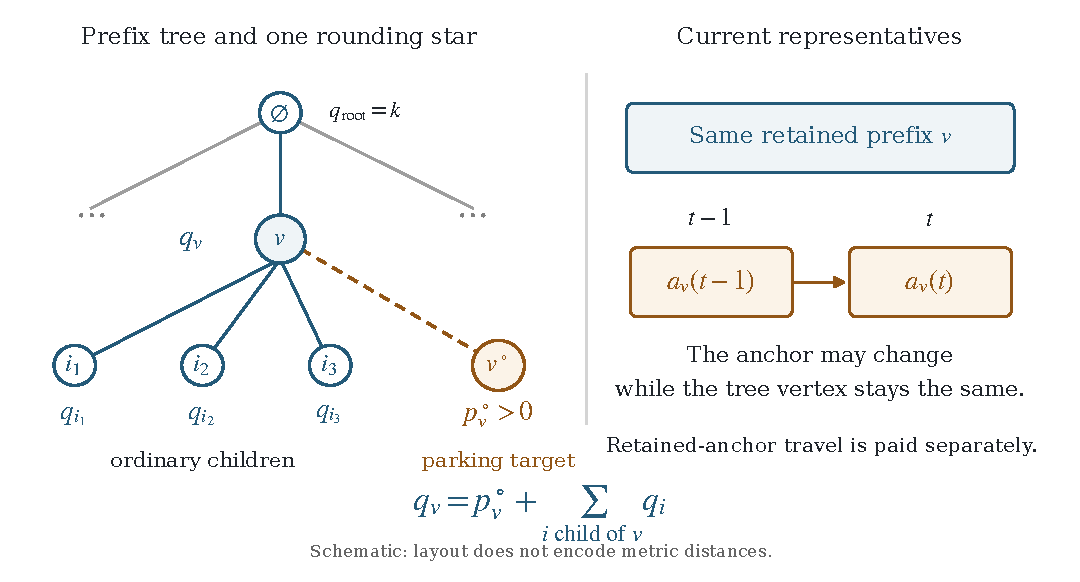
\includegraphics[width=.94\textwidth]{figures/parked_tree.pdf}
 \caption{A subtree amount is split between its children and a park at
 its own vertex. The park is included as one more child target during
 rounding. A fixed tree vertex can have a moving representative in
 the original metric, so its parked mass requires a separate travel
 estimate. The picture records conservation and does not assert that
 the original metric is a Euclidean tree.}
 \label{fig:parked-tree}
\end{figure}

Let \(P\) be expected movement of the mapped hidden comparator on tree
leaves, and put
\[
       V=\E\sum_t\sum_{v\ne\mathrm{root}}
                     r_{|v|-1}|\Delta q_v|.
\]
The main estimates are
\begin{align*}
 P&\le C\ell Q+B_P,\\
 V&\le C\ell P+B_V,\\
 \E\,\cost_{\mathrm{sim}}
   &\le C(V+\ell P+\ell Q)+B_T.
\end{align*}
Their additive terms have the uniform meaning specified above.
Figure~\ref{fig:budget-flow} displays their dependence.

\begin{figure}[!htbp]
 \centering
 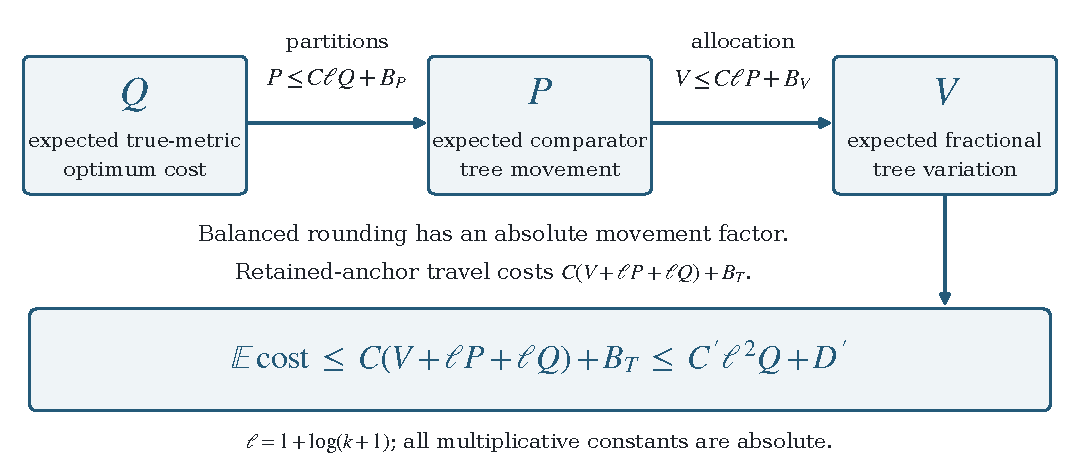
\includegraphics[width=.98\textwidth]{figures/budget_flow.pdf}
 \caption{Movement accounting. The partitions and the tree allocation
 each contribute one logarithm. Rounding has an absolute loss.
 Moving the representatives costs \(O(V+\ell P+\ell Q)\), so it
 preserves the final squared logarithm. All additive terms shown
 are uniform in the finite input law and horizon.}
 \label{fig:budget-flow}
\end{figure}


\section{Allocation on a separated tree: rank data}
\label{sec:allocation}

We first solve an allocation problem on a fixed finite tree.  The allocation
uses conditional distributions of hidden subtree counts.  Convex functions
of their rank probabilities give compatible lower bounds on the amounts
allocated to subtrees.  A small, size-dependent change in the functions
provides the slack needed to move those amounts slowly.

Let $\mathcal T$ be a finite rooted tree whose leaves have depth $J$.
Write $|v|$ for depth and $i\prec v$ when $i$ is a child of $v$.
Fix $r_j=r_0\tau^{-j}$, where $r_0>0$ and $\tau\ge2$.
Write $d_T$ for the leaf metric: distinct leaves with last common
ancestor of depth $j$ have distance $r_j$.  At time $t$ there are $k$
labeled hidden members at leaves,
and a leaf $x_t$ known to $\mathcal F_t$ is required.  Assume that,
conditional on $\mathcal F_t$, at least one hidden member is at $x_t$
with probability one.  Let $N_v(t)$ be the number in the subtree of $v$,
and put $m_v(t)=\E[N_v(t)\mid\mathcal F_t]$.  The expected sum of
the labeled members' successive traveled distances is denoted by $P$;
it includes their movement from time zero.  All conditional distributions
below are available from the observed history.

\begin{theorem}[Dominated tree allocation]\label{thm:allocation}
There are absolute constants $C_0,C_1$ and $\tau_0$ with the following
property.  For $\tau\ge\tau_0$, the observed histories determine amounts
$q_v(t)$ satisfying
\begin{equation}\label{eq:allocation-constraints}
 q_{\mathrm{root}}=k,\qquad
 0\le q_v\le C_0m_v,\qquad
 \sum_{i\prec v}q_i\le q_v,\qquad q_{x_t}\ge1.
\end{equation}
Moreover, with $\ell=1+\log(k+1)$,
\begin{equation}\label{eq:allocation-bound}
 V:=\E\sum_{t\ge1}\sum_{v\ne\mathrm{root}}
       r_{|v|-1}|q_v(t)-q_v(t-1)|
 \le C_1\ell P+D_{\mathcal T}.
\end{equation}
Here sums stop at the chosen finite horizon.  The finite constant
$D_{\mathcal T}$ depends only on the fixed tree, radii, and $k$;
it can be chosen independently of the input law, horizon, and number of
histories.  No initial allocation is prescribed.
\end{theorem}

The proof occupies Sections~\ref{sec:allocation}--\ref{sec:allocation-finish}.

At a vertex $v$, the local task is to distribute its amount $q_v$ among
the children without violating their serving lower bounds.  We construct
child allowances $d_i$, then remove at least $(\sum_i d_i-q_v)_+$ from
them; additional removals leave mass parked at $v$.  The removal choices
must remain stable under posterior fluctuations.  Section~\ref{sec:proportions}
constructs these choices, and Section~\ref{sec:allocation-finish} proves
that the resulting allocations meet their lower bounds and move slowly.

This section supplies the rank lower bounds and the allowances.  It uses
coarse estimates to control changes of the removal rule's parameters,
and finer estimates for the final allowances.  Only the coarse variation
will be multiplied by logarithmic potential slopes; keeping these two
budgets separate preserves the single factor of $\ell$ in the theorem.

Rank coordinates for subtree occupancies also occur in the assignment
polytope of \cite[Section~3.2]{BCLLM18}. Here they are probabilities of
the hidden comparator's occupancies, conditional on the observed history.
For $1\le a\le k$, define the rank probabilities and their filtered values by
\[
 p_{va}(t)=\Pr(N_v(t)<a\mid\mathcal F_t),\qquad
 p^-_{va}(t)=\Pr(N_v(t-1)<a\mid\mathcal F_t).
\]
Thus $\E[p^-_{va}(t)\mid\mathcal F_{t-1}]=p_{va}(t-1)$.
The drift of this coordinate is
$\delta_t p_{va}=p_{va}(t)-p^-_{va}(t)$, rather than its entire change
between successive observations.  For the star at an internal vertex $v$,
put
\begin{equation}\label{eq:star-drift}
 E_v=\E\sum_{t\ge1}\left(
        \sum_{i\prec v}\sum_{a=1}^k|\delta_t p_{ia}|
             +\sum_{a=1}^k|\delta_t p_{va}|\right).
\end{equation}
These local budgets satisfy
\begin{equation}\label{eq:rank-drift-tree}
             \sum_{v\text{ internal}}r_{|v|}E_v\le6P.
\end{equation}
Indeed, for two integer counts $n,n'\in\{0,\ldots,k\}$,
\[
 \sum_{a=1}^k|\one_{\{n<a\}}-\one_{\{n'<a\}}|=|n-n'|.
\]
Use the coupling of successive hidden configurations and conditional
expectation to bound each rank drift by the corresponding indicator
change.  A nonroot vertex of depth $d$ receives weight at most
$r_{d-1}+r_d$ when all stars are summed.  If one labeled member moves
between leaves with last common ancestor of depth $j$, its indicators
change on the two paths strictly below that ancestor.  Its total charge
is at most
\[
 2\sum_{d=j+1}^J(r_{d-1}+r_d)
 \le\frac{2(1+\tau^{-1})}{1-\tau^{-1}}r_j\le6r_j.
\]
The root count is constant.  Summing over the members proves
\eqref{eq:rank-drift-tree}.

\subsection{Explicit rank functions and compatible lower bounds}

\begin{lemma}[Rank functions]\label{lem:rank-functions}
There are absolute constants $p_*,s_*,\epsilon_*>0$, with $p_*<s_*<1$,
and functions $l^\beta:[0,1]\to[0,1]$ for
$3\le\beta\le3+\epsilon_*$ such that:
\begin{enumerate}
\item $l^\beta$ is convex and nonincreasing, equals $1-\beta p$ on
      $[0,p_*]$, is positive on $[0,s_*)$, and is zero on $[s_*,1]$;
\item $l^\beta$ is affine and nonincreasing in $\beta$, and the square
      roots $\sqrt{l^\beta}$ have a common absolute Lipschitz constant;
\item if $g(p)=-\partial_\beta l^\beta(p)$, then
\begin{equation}\label{eq:rank-derivative}
 \frac1{96}l^\beta(p)\le g(p)\le l^\beta(p)
       \qquad(p\in[p_*/4,1]).
\end{equation}
\end{enumerate}
One may take $p_*=1/24$, $s_*=5/8$, and $\epsilon_*=1/100$.
\end{lemma}

\begin{proof}
Set $t_*=s_*-p_*=7/12$ and
\[
 A_*=\frac{18}{7},\qquad c_*'=\frac6{49},\qquad
 d_*'=\frac{1152}{343},\qquad b_*'=c_*'+d_*'t_*=\frac{102}{49}.
\]
For $0\le z\le1/100$ define
\begin{equation}\label{eq:explicit-rank}
 l^{3+z}(p)=
 \begin{cases}
  1-(3+z)p,&0\le p\le p_*,\\
  (s_*-p)^2\bigl[A_*-z(c_*'+d_*'(p-p_*))\bigr],
                                     &p_*\le p\le s_*,\\
  0,&s_*\le p\le1.
 \end{cases}
\end{equation}
The identities
\[
 A_*t_*^2=1-3p_*,\quad 2A_*t_*=3,\quad
 c_*'t_*^2=p_*,\quad -2c_*'t_*+d_*'t_*^2=1
\]
show that both values and first derivatives match at $p_*$.
They also show that $g$ is $p$ on the first interval and
$(s_*-p)^2(c_*'+d_*'(p-p_*))$ on the second.

Writing $x=s_*-p$, the middle expression for $l^{3+z}$ is
\[
            (A_*-zb_*')x^2+zd_*'x^3.
\]
Its two coefficients are nonnegative, with $A_*-zb_*'>2$.
Consequently it is positive before the cutoff, has nonpositive
$p$-derivative, and has positive second derivative.  Its value and
first derivative are zero at the cutoff.  Together with the matching
at $p_*$, this proves global convexity and monotonicity.
On the first interval the function is bounded away from zero, so its
square root has bounded derivative.  On the middle interval its square
root is
$x\sqrt{A_*-zb_*'+zd_*'x}$, which also has bounded derivative,
uniformly in $z$.  The matching and cutoff give the global Lipschitz bound.

For $p\in[p_*/4,p_*]$, the quotient
$g(p)/l^{3+z}(p)=p/(1-(3+z)p)$ lies between $1/96$ and $1$.
On the middle interval the quotient is
\[
 \frac{b_*'-d_*'x}{A_*-zb_*'+zd_*'x},\qquad 0<x\le t_*.
\]
It is at least $c_*'/A_*=1/21$ and at most
$b_*'/(A_*-(1/100)b_*')<1$.  Beyond the cutoff both functions vanish.
This proves \eqref{eq:rank-derivative}.
\end{proof}

Fix also the broader size function
\[
 l^{\mathrm{siz}}(p)=\frac{(3/4-p)_+^2}{(3/4)^2},\qquad
 L_v^\beta=\sum_{a=1}^k l^\beta(p_{va}),\qquad
 M_v=\sum_{a=1}^k l^{\mathrm{siz}}(p_{va}).
\]
Its square root is Lipschitz.  Both kinds of functions vanish at one
and have value one at zero.

The next comparison is a majorization argument in the sense of
Karamata \cite{Karamata32}. We include the convex-hinge proof to specify
the direction of the comparison and the role of the padded coordinates.

\begin{lemma}[Superadditivity]\label{lem:superadditivity}
For every internal vertex $v$ and every allowed $\beta$,
\begin{equation}\label{eq:rank-superadditivity}
 \sum_{i\prec v}L_i^\beta\le L_v^\beta,\qquad
 \sum_{i\prec v}M_i\le M_v\le m_v.
\end{equation}
No independence between child counts is required.
\end{lemma}

\begin{proof}
Suppose there are $d$ children.  Pool their $dk$ rank probabilities
and sort them increasingly, obtaining a vector $x$.
Let $y$ be the parent's $k$ increasingly ordered rank probabilities
followed by $(d-1)k$ ones.  Their total sums agree and equal $dk-m_v$.
If the first $n$ coordinates of $x$ contain $n_i$ coordinates from child
$i$, those coordinates can be chosen as the first $n_i$ of that child.
Since $N_v=\sum_iN_i$, conditional expectation gives
\[
 \sum_{b=1}^n x_b
 =\sum_i\E[(n_i-N_i)_+\mid\mathcal F_t]
 \ge\E[(n-N_v)_+\mid\mathcal F_t]
 =\sum_{b=1}^n y_b.
\]
The last identity also holds for $n>k$, precisely because of the padding.
For every real $b$, an increasing vector $z$ satisfies
\[
       \sum_a(b-z_a)_+
       =\max_{0\le n\le dk}\left(nb-\sum_{a=1}^n z_a\right).
\]
Thus the sum of every convex hinge $(b-p)_+$ on $x$ is no larger
than its sum on $y$.  Affine functions have equal sums.  Every convex
piecewise linear function is an affine function plus a nonnegative
linear combination of these hinges.  Approximating a continuous convex
function by its linear interpolants proves the same comparison for
that function.  Apply it to $l^\beta$ and $l^{\mathrm{siz}}$;
the padded ones contribute zero.  Finally convexity and the endpoint
values give $l^{\mathrm{siz}}(p)\le1-p$, and
$\sum_a(1-p_{va})=m_v$.
\end{proof}

From now on set $c_*=10^{-4}$; thus
$100c_*<l^{\mathrm{siz}}(s_*)=1/36$.  Choose an absolute $c_\beta>0$
so small that
$c_\beta(1+\log(1/c_*))\le\epsilon_*/2$, and define
\begin{equation}\label{eq:vertex-beta}
 \beta_v=3+\frac{c_\beta}{\ell}
                \log\frac{k}{\max(M_v,c_*)}.
\end{equation}
It belongs to $[3,3+\epsilon_*/2]$, because $M_v\le k$ and
$\log(k/c_*)/\ell\le1+\log(1/c_*)$.
The invariant propagated down the tree will be
\begin{equation}\label{eq:allocation-lower-bound}
                         q_v\ge L_v^{\beta_v}.
\end{equation}
Superadditivity gives compatible child lower bounds at the parent's
parameter $\beta_v$.  Since $M_i\le M_v$, the child's own parameter
satisfies $\beta_i\ge\beta_v$, and its required bound is no larger.
The resulting difference is the slack available for choosing slowly
varying child amounts.  We will estimate this difference in terms of
the relative child sizes.
At the root all ranks are zero, $M_{\mathrm{root}}=k$, and the lower
bound is $k$.  At a required leaf $p_{v1}=0$, so the lower bound is
at least one.

\subsection{A rank tracker with a bounded affine potential}

The input to a star may fluctuate substantially when information is
revealed.  The following tracker charges only drift, using signed
filtering changes before it decides whether to refresh.

\begin{lemma}[Rank tracking]\label{lem:rank-tracking}
Let $p_t,p_t^-\in[0,1]$ obey
$\E[p_t^-\mid\mathcal F_{t-1}]=p_{t-1}$, and let
$\mathcal E=\E\sum_t|p_t-p_t^-|$.
If $f\ge0$ has an absolutely bounded Lipschitz constant for $\sqrt f$,
then for $0<\xi<1/2$ there is a held estimate $\widehat f_t$ with
\begin{equation}\label{eq:rank-relative-tracker}
 (1+\xi)^{-1}f(p_t)\le\widehat f_t\le(1+\xi)f(p_t),\qquad
 \E\sum_t|\widehat f_t-\widehat f_{t-1}|
       \le\frac{C}{\xi}(\mathcal E+1).
\end{equation}
In particular zeros are tracked exactly.  A held estimate
$\widehat p_t$ refreshed when $|p_t-\widehat p_{t-1}|>\delta$
has expected number of refreshes at most
$\delta^{-2}(\mathcal E+1)$.
\end{lemma}

\begin{proof}
Initialize a reference $p^\circ=p_0$ and hold $f(p^\circ)$ until
the displayed factor comparison fails, then replace $p^\circ$ by
$p_t$.  With the reference held, use
\[
 \Phi(p;p^\circ)=p(1-p)+(p-p^\circ)^2
              =(1-2p^\circ)p+(p^\circ)^2.
\]
This is affine in $p$, lies in $[0,1]$, and has slope of absolute
value at most one.  At every step, first evaluate its change from
$p_{t-1}$ to $p_t^-$ and then from $p_t^-$ to $p_t$, holding the old
reference.  The former change has conditional expectation zero, and
the latter is at most $|p_t-p_t^-|$.  A reference reset then decreases
$\Phi$ by exactly $(p_t-p^\circ)^2$.  Telescoping gives
\begin{equation}\label{eq:rank-reset-credit}
        \E\sum_{\text{resets}}(p_t-p^\circ)^2\le\mathcal E+1.
\end{equation}

For two nonnegative values $a,b$ failing factor $1+\xi$ comparison,
\[
 (\sqrt a-\sqrt b)^2
 =|a-b|\frac{|\sqrt a-\sqrt b|}{\sqrt a+\sqrt b}
 \ge \frac{\xi}{5}|a-b|.
\]
The inequality includes the case in which exactly one value is zero.
The Lipschitz bound for $\sqrt f$ therefore implies
$(p_t-p^\circ)^2\ge c\xi|f(p_t)-f(p^\circ)|$ at every reset,
proving \eqref{eq:rank-relative-tracker}.  The same potential proves
the absolute-threshold claim, since every reset then releases more
than $\delta^2$.  Filtering was evaluated at every step before the
reset test; no expectation was restricted to a selected reset event.
\end{proof}

Apply the absolute tracker with threshold $p_*/8$ to every child rank.
A rank is called \emph{core} when its held estimate is at most $p_*/2$.
After the update, every core rank has $p\le5p_*/8$, every noncore
rank has $p>3p_*/8$, and every rank with $p<p_*/4$ is core.
Let $K_t$ count the changed core flags in this star at step $t$, and set
\begin{equation}\label{eq:core-data}
 n_i=\#\{a:\text{$a$ is core at $i$}\},\quad
 B_i=\sum_{a\text{ core at }i}p_{ia},\quad
 S=\sum_iB_i,\quad
 f_i^\beta=\sum_{a\text{ noncore at }i}l^\beta(p_{ia}).
\end{equation}
We call \(f_i^\beta\) the \emph{noncore}, or \emph{flex}, contribution.
The core ranks lie in the affine part of every rank function, so
\begin{equation}\label{eq:core-decomposition}
 L_i^\beta=n_i-\beta B_i+f_i^\beta,\qquad
       n_i+\sup_\beta f_i^\beta\le C M_i.
\end{equation}
For the second bound, a core rank contributes at least
$l^{\mathrm{siz}}(5p_*/8)>0$ to $M_i$.  Any positive $l^\beta(p)$
has $p<s_*$, where $l^{\mathrm{siz}}(p)\ge1/36$ and $l^\beta(p)\le1$.
These termwise bounds prove the assertion with an absolute constant.
In particular,
\begin{equation}\label{eq:inactive-rank-vanishing}
 M_i\le10c_*\quad\Longrightarrow\quad
 n_i=0\ \text{ and }\ L_i^\beta=f_i^\beta=0\ \text{for all $\beta$}.
\end{equation}
Also, if the old flags are held while the ranks are filtered and drifted,
the resulting old-flag sum always satisfies $B_i\le n_i^{\mathrm{old}}$,
even if those old flags no longer describe small current probabilities.
This elementary bound will be used at wholesale changes.

\subsection{Coarse data, active epochs, and parameter gaps}

We now describe a schedule local to a star.  Its estimates are computed
from the final, post-filtering and post-drift, ranks on each step.
All elementary term trackers persist throughout the entire process,
including times when a child is inactive and times when the schedule
below is restarted.

Choose a sufficiently small absolute size tolerance $\delta_s>0$,
for example $10^{-3}$.  Track every term of $M_i$ by
Lemma~\ref{lem:rank-tracking} with this tolerance, and let
$\widehat M_i$ be their sum.  A child is either inactive, with $a_i=0$,
or active.  Turn an inactive child on when $\widehat M_i\ge5c_*$,
setting $a_i=\widehat M_i$.  Turn an active child off when
$\widehat M_i\le2c_*$.  Otherwise, during an active period hold $a_i$
until factor $1+\delta_s$ comparison with $\widehat M_i$ fails,
then replace $a_i$ by $\widehat M_i$.  Initialize with the same rules,
using either admissible state in the overlap.  These choices ensure
\begin{equation}\label{eq:active-size-accuracy}
 \begin{gathered}
 0.9M_i\le a_i\le1.1M_i\quad\text{at active children},\qquad
 M_i\ge c_*\quad\text{if active},\\
 M_i\ge10c_*\quad\Longrightarrow\quad\text{active}.
 \end{gathered}
\end{equation}
By \eqref{eq:inactive-rank-vanishing}, an inactive child has no core
ranks or positive rank lower bounds.

We also hold an accurate estimate of $X_v=\max(M_v,c_*)$.
For this purpose take a possibly smaller absolute tolerance $\delta_p$,
track the parent size terms, and clip their sum below at $c_*$,
obtaining $\widehat X_v$.  Hold $H_v$ equal to its last reference value,
refreshing upon failure of factor $1+\delta_p$ comparison.  Then
\[
 (1+\delta_p)^{-2}X_v\le H_v\le(1+\delta_p)^2X_v.
\]
Put
\begin{equation}\label{eq:held-beta-upper}
 X_v^{\mathrm{low}}=\max\{c_*,H_v/(1+\delta_p)^2\},\qquad
 \beta^+=3+\frac{c_\beta}{\ell}\log\frac{k}{X_v^{\mathrm{low}}}.
\end{equation}
Here $X_v^{\mathrm{low}}\le X_v\le k$, and
$X_v^{\mathrm{low}}\ge X_v/(1+\delta_p)^4$.  Thus, for any prescribed
small absolute $\epsilon>0$, choosing $\delta_p$ sufficiently small gives
\begin{equation}\label{eq:beta-upper-error}
       \beta_v\le\beta^+\le\beta_v+\epsilon/\ell.
\end{equation}
The parameter stays in the allowed interval and changes only when
$H_v$ is refreshed.

An \emph{epoch} starts with a \emph{wholesale change}, performed initially
and whenever $\beta^+$ changes or the cumulative $\ell_1$ variation of
the held size vector since the epoch started exceeds $A/100$.
Here $A=\sum_i a_i$ at the start is held for that epoch.  Empty to
nonempty or nonempty to empty changes always start a new epoch.
At a wholesale change, choose a dominant index $o$ if some
$a_o\ge0.85A$ and $A>0$.  It is unique.  Keep that mark until the
next wholesale change.  All other active indices, or all active indices
when there is no mark, are called regular.  With a dominant index the
regular indices are also called sides.  No elementary size or rank
tracker is restarted at an epoch boundary.

During a marked epoch, let $T_{\mathrm{side}}=\sum_{i\ne o}a_i$.
Set $U=T_{\mathrm{side}}$ at its start.  Subsequently hold $U$ until
factor $1+\delta_s$ comparison with $T_{\mathrm{side}}$ fails, then
refresh it to that side total.  This includes transitions to or from zero.
When sides exist set $u=U/A$; otherwise set $u=0$.  For active children
define
\begin{equation}\label{eq:gap-weights}
 h_i=1+\max\{0,\log(A/a_i)\}\quad(i\text{ regular}),\qquad
 h_o=u\quad(o\text{ dominant}).
\end{equation}
The empty active domain needs none of these parameters.

Finally prepare a coarse scale for a marked child.  Independently of
the fine estimates used below, track every child rank value
$l^3(p_{ia})$ with tolerance $\delta_s$, and write its estimate as
$\widehat l^{\mathrm{coarse}}_{ia}$.  With a dominant index set
\begin{equation}\label{eq:dominant-scale-definition}
             D=\sum_{a\text{ noncore at }o}
                       \widehat l^{\mathrm{coarse}}_{oa};
\end{equation}
set $D=0$ when no dominant index exists.  All these term trackers run
on every child and every rank even when their estimates are not currently
used in $D$.

Here is a precise inventory of the coarse charges.  Write
$a_i^-,a_i^+$ for the old and new held sizes on a step, and similarly
for other held quantities; these superscripts in this inventory refer
to step-end states, not to the filtered hidden configuration.
Let $\mathcal W_v$ be the wholesale steps after initialization,
$\mathcal H_v$ the steps at which $H_v$ is refreshed, and
$\mathcal U_v$ the non-wholesale steps at which $U$ is refreshed.
Define the nonnegative charge
\begin{equation}\label{eq:coarse-charge-definition}
\begin{aligned}
 C_{v,t}={}&K_t+
    \sum_{i:a_i^-\ne a_i^+}(a_i^-+a_i^+)
    +\one_{\{t\in\mathcal H_v\}}(H_v^-+H_v^+)\\
 &+\one_{\{t\in\mathcal W_v\}}\sum_i(a_i^-+a_i^+)
    +\one_{\{t\in\mathcal U_v\}}
                    (T_{\mathrm{side}}^-+T_{\mathrm{side}}^+)
    +|D^+-D^-|.
\end{aligned}
\end{equation}
The side totals in this expression use the unchanged dominant mark
on a non-wholesale step.  A wholesale change of $U$, including a
change of mark, is covered by the wholesale total in the preceding term.

\begin{lemma}[Coarse budgets and parameter gaps]\label{lem:parameter-gaps}
The data above satisfy, for an absolute constant $C$ and a finite
$D_v^{\mathrm{data}}$ depending only on the fixed star and $k$,
\begin{equation}\label{eq:coarse-data-budget}
             \E\sum_t C_{v,t}\le C E_v+D_v^{\mathrm{data}}.
\end{equation}
The constant is uniform in the law and horizon.  Every active child obeys
\begin{equation}\label{eq:parameter-gap}
        0\le h_i\le C\ell,\qquad
        \beta_i-\beta_v\ge\frac{c_g h_i}{\ell}
\end{equation}
for an absolute $c_g>0$.  If a dominant index and sides are present,
then $0<u<1/4$, and with $H=1+\log(1/u)$ every side satisfies
$h_i\ge cH$ for an absolute $c>0$.
In addition, $n_i+B_i+\sup_\beta f_i^\beta\le C a_i$ at active
children, and all these quantities vanish at inactive children.
\end{lemma}

\begin{proof}
We give the amortization details because paying a large size on every
small refresh would not suffice.  Lemma~\ref{lem:rank-tracking}, summed
over the fixed collection of size terms, bounds the expected total
variation of their estimates by $CE_v$ plus a fixed initialization
constant.  It bounds $\E\sum_tK_t$ in the same way.  Constants may depend
on the fixed absolute tolerances but never on $k$ or the degree.

For a scalar estimate $x$ held at a reference $b>0$, a factor
$1+\delta$ failure gives
\[
             b+x\le(1+2/\delta)|x-b|.
\]
The last difference is bounded by the variation of $x$ since its previous
reference setting; these intervals are disjoint.  This pays all active
to active changes of $a_i$ and all changes of $H_v$.
Turning a child on after an off period costs its new size, and is paid
by the variation from a previous value at most $2c_*$ to a value at least
$5c_*$.  The first such event may instead use an initialization charge.
For a turn-off, if the last held size exceeds $4c_*$, variation since
that setting pays it because the new estimate is at most $2c_*$.
Otherwise the charge is at most $4c_*$ and is paid by the traversal
from at least $5c_*$ at the start of this on period to at most $2c_*$
at its end.  Each on period and each off period is used only once in
these latter arguments.  They overlap the scalar refresh intervals
only a bounded number of times.  This proves the budget for all
changed-$a_i$ charges.  Clipping the parent sum below at $c_*$ does
not increase its variation, so the same argument applies to $H_v$.

When $\beta^+$ changes, the old and new active totals are at most
$C(X_v^-+X_v^+)\le C(H_v^-+H_v^+)$, and are therefore paid by that
parent refresh.  For a wholesale event from the vector-variation test,
let $R$ be the cumulative variation since the previous epoch started
and let $A$ be that epoch's initial total.  The old total is at most
$1.01A$, the new total is at most $1.01A+R$, and $R>A/100$.
Their sum is consequently at most $203R$.  The intervals of variation
assigned to successive epochs are disjoint.  If $A=0$, the new total
is at most $R$, and the same conclusion holds.  Discarding unused
variation credit when a parent refresh intervenes cannot increase its
total use.  This proves the wholesale budget.

On a fixed marked epoch, variation of $T_{\mathrm{side}}$ is at most
$\sum_i|\Delta a_i|$.  The scalar relative-refresh argument pays every
$U$ refresh by variation since its previous setting.  The actual old
side total is within factor $1+\delta_s$ of that reference, so the
old plus new side totals have the same bound.  A zero crossing is
included: the variation then pays the positive reference or positive
new total.  Setting $U$ at a wholesale change is paid by the wholesale
total.  Thus all its asserted charges are covered.

At a non-wholesale step the dominant index is unchanged.  The variation
of \eqref{eq:dominant-scale-definition} is at most the summed variation
of its coarse term estimates plus $CK_t$: a changed flag inserts or
removes one term, each at most one.  At a wholesale step, its old and
new values are at most $C(a_o^-+a_o^+)$, interpreted as zero when that
mark is absent; this follows from the relative estimates and
\eqref{eq:core-decomposition}.  The wholesale totals pay these changes.
This proves \eqref{eq:coarse-data-budget}.

For the gaps, at every state of an epoch with $A>0$ the current active
total is in $[0.99A,1.01A]$.  In an unmarked epoch every child has
$a_i\le0.86A$.  In a marked epoch the marked size is at least $0.84A$,
and the side total is at most $0.16A$; in particular the mark stays
active.  Therefore every regular child has $a_i\le0.86A$.
By \eqref{eq:active-size-accuracy} and superadditivity,
\begin{equation}\label{eq:size-log-comparison}
 \frac{M_v}{M_i}\ge
 1+\frac9{11}\frac{\sum_{j\ne i,\ a_j>0}a_j}{a_i}
 \ge1+\frac9{11}\left(\frac{0.99A}{a_i}-1\right).
\end{equation}
For $x=A/a_i\ge1/0.86$, the logarithm of the last expression is
at least $c(1+\log x)$ for an absolute $c>0$.  To see the uniformity,
the ratio to $1+\log x$ is continuous and positive on this interval
and tends to one as $x\to\infty$; on a sufficiently large tail it is
at least $1/2$, and on the remaining compact interval it has a
positive minimum.  This proves the regular comparison.
For the dominant child, use the first inequality in
\eqref{eq:size-log-comparison}, the comparisons
$T_{\mathrm{side}}\asymp U$, and $a_o\le1.01A$ to obtain
\[
                 \log(M_v/M_o)\ge cU/A=cu.
\]
Here $u\le(1+\delta_s)0.16<1/4$, so $\log(1+cu)\ge c'u$.
If no sides exist, $u=0$ and the claimed inequality is automatic.

At every active child $M_i\ge c_*$ and $M_v\ge M_i$, so the clipping
in \eqref{eq:vertex-beta} is inactive at both vertices.  Hence
\[
               \beta_i-\beta_v
                  =\frac{c_\beta}{\ell}\log(M_v/M_i),
\]
which proves the gap in \eqref{eq:parameter-gap}.
Active held sizes have an absolute positive lower bound and
$A\le1.1k$, proving $h_i\le C\ell$.  On a side,
$a_i\le T_{\mathrm{side}}\le(1+\delta_s)uA$, whence
\[
 h_i\ge1+\log(1/u)-\log(1+\delta_s)\ge H/2.
\]
The final bounds on core and flex data follow from
\eqref{eq:core-decomposition}, $B_i\le n_i$, and
\eqref{eq:active-size-accuracy}.  Inactivity was addressed in
\eqref{eq:inactive-rank-vanishing}.
\end{proof}

\subsection{Fine caps and their separate budget}

The proportions constructed in the next section will use only the
coarse data above and the raw core sums $B_i$.  The following finer
estimates enter only the final allocations.  Keeping their variation
out of the proportion potentials is necessary for the single factor
of $\ell$ in Theorem~\ref{thm:allocation}.

The parameter gap at a regular child leaves room to track its flex
contribution between $f_i^{\beta_i}$ and $f_i^{\beta_v}$.  A marked
child can have an arbitrarily smaller gap as its side mass tends to
zero.  We therefore use a small upper approximation at that child;
Section~\ref{sec:proportions} explains how this asymmetry changes the
removal rule.

\begin{lemma}[Caps]\label{lem:caps}
Given a sufficiently small absolute $\epsilon_b>0$, the remaining
absolute tolerances can be chosen so that there are caps
$d_i=n_i+b_i$, zero on inactive children, with
\begin{equation}\label{eq:cap-feasibility}
 \begin{aligned}
 f_i^{\beta_i}\le b_i\le f_i^{\beta_v}
                                      &&(i\text{ regular}),\\
 T:=f_o^{\beta_v}\le b_o\le(1+\epsilon_b/\ell)T,
 \qquad c_DT\le D\le C_DT
                                      &&(o\text{ dominant}).
 \end{aligned}
\end{equation}
Here $c_D,C_D>0$ are absolute, fixed independently of
$\epsilon_b$ and the fine tolerances; in particular $D=0$ if and only
if $T=0$.  At every child $d_i\le C M_i\le C m_i$.
Their variation away from wholesale changes satisfies
\begin{equation}\label{eq:fine-cap-budget}
 \E\sum_{t\notin\mathcal W_v}\sum_i|d_i(t)-d_i(t-1)|
          \le C\ell E_v+D_v^{\mathrm{cap}},
\end{equation}
where $D_v^{\mathrm{cap}}$ is uniform in the law and horizon.
At wholesale changes the old plus new caps are bounded by $C$ times
the old plus new active totals.
\end{lemma}

\begin{proof}
For every rank, at both endpoint parameters $3$ and $3+\epsilon_*$,
run separate relative trackers with tolerance $\rho/\ell$, where
$\rho>0$ is a small absolute constant to be selected.
Interpolate their estimates by the convex coefficients expressing
$\beta^+$ between these endpoints, and sum over the current noncore
ranks at child $i$.  Call the result $\widetilde f_i$.
The affinity in $\beta$ and the relative endpoint estimates imply
\[
 (1+\rho/\ell)^{-1} f_i^{\beta^+}
       \le\widetilde f_i\le(1+\rho/\ell)f_i^{\beta^+}.
\]
Every noncore rank has $p>3p_*/8$, so
\eqref{eq:rank-derivative} applies to it.  Together with
\eqref{eq:beta-upper-error}, this yields
\begin{equation}\label{eq:flex-estimate-error}
       |\widetilde f_i-f_i^{\beta_v}|
          \le\frac{e}{\ell}f_i^{\beta_v},\qquad
                      e\le C(\rho+\epsilon).
\end{equation}
For example,
$f_i^{\beta_v}-f_i^{\beta^+}
=(\beta^+-\beta_v)\sum_{\mathrm{noncore}}g(p_{ia})
\le(\epsilon/\ell)f_i^{\beta_v}$.
If the true sum is zero then both endpoint estimates, and therefore
the interpolated sum, are exactly zero, since all the functions have
the same cutoff.

For a regular child, $h_i\ge1$ and the parameter gap gives
\begin{equation}\label{eq:regular-flex-slack}
 f_i^{\beta_i}
 =f_i^{\beta_v}-(\beta_i-\beta_v)
                  \sum_{\mathrm{noncore}}g(p_{ia})
 \le(1-\gamma/\ell)f_i^{\beta_v},
             \qquad \gamma=c_g/96>0.
\end{equation}
Choose an absolute
$0<\lambda_b\le\min\{\gamma/4,\epsilon_b/4,1/4\}$,
and then choose $\rho,\epsilon$ so small that the $e$ in
\eqref{eq:flex-estimate-error} is at most $\lambda_b/4$.
Define
\[
 b_i=(1-\lambda_b/\ell)\widetilde f_i\quad(i\text{ regular}),
 \qquad
 b_o=(1+\lambda_b/\ell)\widetilde f_o\quad(o\text{ dominant}).
\]
For a regular child the upper estimate is at most $f_i^{\beta_v}$,
because $e\le\lambda_b$; the lower estimate is at least
$(1-(\lambda_b+e)/\ell)f_i^{\beta_v}$, which dominates
\eqref{eq:regular-flex-slack}.  For a dominant child,
$(1+\lambda_b/\ell)(1-e/\ell)\ge1$, whereas
$(1+\lambda_b/\ell)(1+e/\ell)\le1+\epsilon_b/\ell$.
This proves the cap comparisons.

On the noncore range \eqref{eq:rank-derivative} also gives
\[
 l^{\beta_v}\le l^3
       =l^{\beta_v}+(\beta_v-3)g
       \le(1+\epsilon_*)l^{\beta_v}.
\]
The coarse tracker defining $D$ therefore satisfies
\[
 (1+\delta_s)^{-1}T\le D
       \le(1+\delta_s)(1+\epsilon_*)T.
\]
These choices give the claimed $c_D,C_D$ and show that their values
precede all fine choices.  The bound $d_i\le C M_i$ follows from
\eqref{eq:core-decomposition} and the relative estimates.

It remains to account for variation.  Lemma~\ref{lem:rank-tracking}
with tolerance $\rho/\ell$ pays the summed variation of all endpoint
estimates by $C\ell E_v$ plus a fixed constant.  On a non-wholesale
step, $\beta^+$ and the dominant mark are unchanged, so their
interpolation coefficients and the factors $1\pm\lambda_b/\ell$
are fixed.  Changes of the noncore sets cost at most $CK_t$, as does
the variation of $n_i$.  An inactive child has zero true endpoint
values and hence zero endpoint estimates; setting its cap to zero
therefore adds no variation beyond the same term and flag changes.
This proves \eqref{eq:fine-cap-budget}.  At a wholesale step,
$d_i^-+d_i^+\le C(a_i^-+a_i^+)$, including zero inactive values,
and summing proves the remaining statement.
\end{proof}

All the additive terms in this section arise from bounded potentials
and bounded initialization charges for a fixed number of rank trackers.
There are only $k$ ranks per vertex of the fixed finite tree.
The term trackers are never reinitialized when an epoch changes or a
tree label reappears.  Thus their total additive allowance is uniform
over every law and horizon.  The coarse allowance
\eqref{eq:coarse-data-budget} and the fine allowance
\eqref{eq:fine-cap-budget} are separate: only the former will be
multiplied by the $O(\ell)$ slopes of the next section's potentials.

The remaining construction starts from the caps $d_i$ and distributes
the required reduction $\bigl(\sum_i d_i-q_v\bigr)_+$ between children.
The star's parameters, flags, and proportion trackers can all be
updated from its own rank inputs before $q_v$ is known.  The actual
allocations are then propagated from the root downwards.

\section{Slow proportions with changing domains}
\label{sec:proportions}

We continue the construction at one fixed star $v$, using the parameters
of Lemmas~\ref{lem:parameter-gaps} and~\ref{lem:caps}.
The caps $d_i$ will be reduced to fit the parent amount.  This section
constructs proportions for those reductions.  The construction depends
only on the star's observed rank posteriors and held parameters; the
parent amount $q_v$ is not an input.

Write $I$ for the active children, and extend all vectors by zero to the
fixed set of children when comparing different times.  Recall that
$B_i$ is the sum of the current rank probabilities over the core flags,
$S=\sum_i B_i$, and inactive children have no core flags.
If a dominant child $o$ is marked, the other active children are called
sides.  For regular children and for a marked child with sides,
respectively, the held parameters satisfy
\begin{equation}\label{eq:proportion-parameter-facts}
\begin{gathered}
  1\le h_i\le C\ell\quad(i\text{ regular}),\qquad
  h_o=u=U/A\in(0,1),\qquad H=1+\log(1/u),\\
  h_i\ge cH\quad(i\text{ a side}),\qquad
  \sum_{i\text{ regular}}e^{-h_i}\le
  \begin{cases} C,&\text{no dominant child},\\ Cu,&\text{a dominant child}.
  \end{cases}
\end{gathered}
\end{equation}
The last assertion follows from $e^{-h_i}\le a_i/A$ and the comparison
of $U$ with the side total.  These facts hold throughout each epoch.
When $I$ is empty there is no proportion to choose.  When $I=\{o\}$,
we use $\alpha_o=1$, $u=h_o=0$, and no side vector.  Both potentials
below are then defined to be zero.  In particular, we never evaluate a
denominator with $u=0$.

\subsection{Removal constraints and the simplex tracker}

Fix a sufficiently small absolute $c_t>0$ and put
$\eta_i=c_t h_i/\ell$.  For a nonempty active domain we require
\begin{equation}\label{eq:alpha-feasibility}
  \alpha_i\ge0,\qquad \sum_{i\in I}\alpha_i=1,
  \qquad S\alpha_i\le(1+\eta_i)B_i\quad(i\in I).
\end{equation}
This is automatic on a singleton domain.

To see the role of the tolerance $\eta_i$, temporarily fix any parent
amount $q_v\ge L_v^{\beta_v}$.  Removing the excess
$R_0=(\sum_i d_i-q_v)_+$ in proportions $\alpha$ would give
$q_i=d_i-R_0\alpha_i$.  The cap bounds and superadditivity imply
\[
 R_0\le\beta_v S+e_o,\qquad
 0\le e_o:=b_o-f_o^{\beta_v}\le\epsilon_b f_o^{\beta_v}/\ell,
\]
where $e_o=0$ without a marked child.  For $S>0$, a regular child's
removal is therefore at most
$(\beta_v+e_o/S)(1+\eta_i)B_i$.  The term $\beta_v B_i$ is
already allowed by the core decomposition
$L_i^{\beta_v}=n_i-\beta_v B_i+f_i^{\beta_v}$.
The parameter gap $\beta_i-\beta_v$ pays the extra coefficient,
provided $S$ is at least a fixed multiple of the dominant flex mass,
which is comparable to $D$.  At the marked child the error $e_o$
itself can be subtracted from its upper cap, since $\alpha_o\le1$.

When $S$ is small relative to $D$, the ratio $e_o/S$ need not be
controlled.  We then choose side removals $\omega_i$ first and give
the marked child the remaining parent amount, capped by $d_o$.
Superadditivity bounds its uncapped remaining amount below by
\[
             L_o^{\beta_v}
                  +\sum_{i\ne o}(\omega_i-\beta_v B_i).
\]
It therefore suffices to bound the total signed shortfall of the side
removals below $\beta_v B_i$ by a small multiple of $uD/\ell$; the
marked child's flex slack pays this error.  The removals must also stay below
$\beta_iB_i$ to preserve the side lower bounds.  The side tracker
below constructs $w$ so that $\omega_i=Dw_i$ has both properties.
Section~\ref{sec:allocation-finish} verifies the two output rules,
including their zero cases, and chooses between them by overlapping
comparisons of $S$ and $D$.

Near dominance also changes the simplex tracker itself.  The marked
child's parameter gap can be only of order $u/\ell$, forcing
$\eta_o=c_tu/\ell$.  Its potential must remain effective as
$u\downarrow0$; the different denominator below ensures this.
We will also normalize its primitive at $\alpha_o=1$, so changing
$u$ costs in proportion to the side sizes rather than the full
dominant size.

On every nonsingleton domain set, for $y\ge0$,
\begin{equation}\label{eq:proportion-denominators}
  F_i(y)=\frac{(h_i+y)^2}{h_i}\quad(i\text{ regular}),
  \qquad F_o(y)=u+Hy(1+y)\quad(o\text{ marked}).
\end{equation}

\begin{lemma}[Uniform denominator estimates]\label{lem:denominators}
For every nonsingleton domain above,
\begin{equation}\label{eq:denominator-estimates}
  \int_0^\infty\frac{dy}{F_i(y)}\le C,
  \qquad
  \sum_{i\in I}\alpha_i F_i\bigl(\log(1/\alpha_i)\bigr)
       \le C\sum_{i\in I}\alpha_i h_i
\end{equation}
for every $\alpha$ in its unit simplex.  A summand at $\alpha_i=0$
means its continuous extension, which is zero.  All constants are
uniform as $u$ tends to zero.
\end{lemma}

\begin{proof}
The regular integral equals $1$.  For the marked child, split at $1$:
\[
 \int_0^1\frac{dy}{u+Hy(1+y)}
   \le \frac{\log(1+H/u)}H,
 \qquad
 \int_1^\infty\frac{dy}{u+Hy(1+y)}\le\frac1H.
\]
Since $\log(1/u)=H-1$ and
$\log(1+H/u)\le H-1+\log(1+H)\le2H$, these bounds are absolute.

For the second assertion put $y_i=\log(1/\alpha_i)$ at positive
coordinates.  If $i$ is regular and $y_i\le4h_i$, its contribution
is at most $25\alpha_i h_i$.  If $y_i>4h_i$, then $h_i\ge1$ and
\[
 e^{-y_i}\frac{(h_i+y_i)^2}{h_i}
       \le C e^{-y_i}y_i^2
       \le C e^{-y_i/2}\le C e^{-h_i}.
\]
Thus the regular tail is at most $C$ without a marked child and at
most $Cu$ with one.  Without a marked child,
$\sum_i\alpha_i h_i\ge1$, which pays this tail.

With a marked child use the elementary inequality
$e^{-y}y(1+y)\le C(1-e^{-y})$, valid for all $y\ge0$.
It follows, including the endpoint $\alpha_o=0$, that
\[
 \alpha_o F_o\bigl(\log(1/\alpha_o)\bigr)
       \le C\{\alpha_o u+H(1-\alpha_o)\}.
\]
By \eqref{eq:proportion-parameter-facts},
$\sum_i\alpha_i h_i$ bounds this last expression up to an absolute
factor.  It also bounds $u$ up to an absolute factor: its dominant
contribution is $\alpha_o u$, and its side contribution is at least
$cH(1-\alpha_o)\ge cu(1-\alpha_o)$.  This pays the regular tail
and completes the proof.
\end{proof}

For held parameters and a nonnegative vector $B$, with
$S=\sum_i B_i$, define
\begin{equation}\label{eq:alpha-primitive}
\begin{aligned}
 g_i^\alpha(a;B)
   &=C_\alpha\ell\int_0^a
       \frac{S-(1+\eta_i)B_i/s}{F_i(\log(1/s))}\,ds
       &&(i\text{ regular}),\\
 g_o^\alpha(a;B)
   &=C_\alpha\ell\int_1^a
       \frac{S-(1+\eta_o)B_o/s}{F_o(\log(1/s))}\,ds,
       &&(o\text{ marked}),\\
 G^\alpha(\alpha;B)&=\sum_{i\in I}g_i^\alpha(\alpha_i;B).
\end{aligned}
\end{equation}
The improper integrals at zero converge by
$y=\log(1/s)$ and Lemma~\ref{lem:denominators}.
Consequently these functions extend continuously to the whole
simplex.  No convexity in $\alpha$ is asserted or needed.

We record the bounds needed when parameters change.  Uniformly in
$\alpha$,
\begin{equation}\label{eq:alpha-input-slopes}
 |G^\alpha(\alpha;B)-G^\alpha(\alpha;\widetilde B)|
       \le C\ell\|B-\widetilde B\|_1.
\end{equation}
Here and below changing $B$ also changes $S$ to its sum.  Indeed the
coefficient of $B_i$ in its own $B_i/s$ integral is bounded by
$C\ell\int_0^\infty dy/F_i(y)$.  The sum of the coefficients of
$S$ in the regular components has absolute value at most
$C\ell\sum_i\alpha_i\le C\ell$, because $F_i\ge h_i\ge1$.
The marked component's $S$ coefficient is bounded by
$C\ell\int_{\alpha_o}^1 ds/(sF_o(\log(1/s)))\le C\ell$.
This proves \eqref{eq:alpha-input-slopes} without a factor depending
on the number of active children.

The component bounds are
\begin{equation}\label{eq:alpha-component-bounds}
\begin{aligned}
 |g_i^\alpha(\alpha_i;B)|
   &\le C\ell(S\alpha_i+B_i) &&(i\text{ regular}),\\
 |g_o^\alpha(\alpha_o;B)|
   &\le C\ell\left(S(1-\alpha_o)+B_{\rm side}+uS\right),
   & B_{\rm side}&=\sum_{i\ne o}B_i.
\end{aligned}
\end{equation}
For the second bound, let $L=\log(1/\alpha_o)$, allowing $L=\infty$.
The change of variables in \eqref{eq:alpha-primitive} gives
\[
 g_o^\alpha(\alpha_o;B)
  =-C_\alpha\ell\int_0^L
       \frac{S(e^{-y}-1)+B_{\rm side}-\eta_o B_o}{F_o(y)}\,dy.
\]
For $0\le y\le L$, the absolute numerator is at most
$S(1-\alpha_o)+B_{\rm side}+\eta_o S$.
Since $\eta_o=c_tu/\ell$, Lemma~\ref{lem:denominators} proves
the bound.  The base point $1$ is responsible for this cancellation;
it permits parameter changes to be charged to side sizes even when
the dominant size is much larger.

\begin{lemma}[Simplex update]\label{lem:alpha-tracker}
Choose $C_\alpha$ sufficiently large after fixing $c_t$.
For any old vector $\alpha^0$ in the same simplex, a global minimizer
\begin{equation}\label{eq:alpha-minimization}
 \alpha^1\in\argmin_\alpha
       \left\{G^\alpha(\alpha;B)+S\|\alpha-\alpha^0\|_1\right\}
\end{equation}
satisfies \eqref{eq:alpha-feasibility} and
\begin{equation}\label{eq:alpha-update-payment}
 S\|\alpha^1-\alpha^0\|_1
       \le G^\alpha(\alpha^0;B)-G^\alpha(\alpha^1;B).
\end{equation}
The same assertions hold with the automatic singleton rule.
\end{lemma}

\begin{proof}
Continuity and compactness give a global minimizer, and comparison
with $\alpha^0$ gives \eqref{eq:alpha-update-payment}.
If $S=0$, then every $B_i=0$, the potential vanishes identically,
and feasibility is automatic.  We may retain $\alpha^0$.
Suppose henceforth that $S>0$ and the domain is nonsingleton.
For a positive coordinate write
\[
 \gamma_i=\frac{C_\alpha\ell}{F_i(\log(1/\alpha_i))}
                  \left(S-\frac{(1+\eta_i)B_i}{\alpha_i}\right)
\]
for the derivative of its primitive.
If $\alpha_i=0$ and $B_i>0$, the inward derivative is $-\infty$:
the negative term has size proportional to
$1/(sF_i(\log(1/s)))$, which tends to infinity as $s\downarrow0$.

There must be a coordinate with derivative less than $-2S$, with
this convention at zero.  Otherwise all zero coordinates have
$B_i=0$, and the inequalities $\gamma_i\ge-2S$ give
\begin{equation}\label{eq:alpha-derivative-contradiction}
 1\le\sum_{\alpha_i>0}\frac{\alpha_i}{1+\eta_i}
       \left(1+\frac{2F_i(\log(1/\alpha_i))}{C_\alpha\ell}\right).
\end{equation}
There is a fixed bound $\eta_i\le\eta_{\max}$, so, with
$T_\alpha=\sum_i\alpha_i h_i$,
\[
 \sum_i\frac{\alpha_i}{1+\eta_i}
    \le1-\frac{c_t}{1+\eta_{\max}}\frac{T_\alpha}{\ell}.
\]
The extra sum in \eqref{eq:alpha-derivative-contradiction} is at
most $CT_\alpha/(C_\alpha\ell)$ by
\eqref{eq:denominator-estimates}.  Choose $C_\alpha$ so this is
less than half the displayed deficit.  Since $T_\alpha>0$ on
every nonsingleton domain, this is a contradiction, however small
$u$ and $T_\alpha$ may be.

If a coordinate violates \eqref{eq:alpha-feasibility}, it is
positive and has strictly positive primitive derivative.  Transfer
a small amount $\varepsilon$ from it to a coordinate whose
derivative is below $-2S$.  These coordinates are distinct and the
transfer stays in the simplex.  The primitive sum decreases at a
rate greater than $2S$, whereas the movement penalty can increase
by at most $2S\varepsilon$.  At a zero receiving coordinate the
one-sided derivative $-\infty$ gives the same strict improvement
for sufficiently small $\varepsilon$.  This contradicts global
minimality and proves feasibility.
\end{proof}

\subsection{The side tracker}

When a dominant child has sides, choose a sufficiently small
absolute $c_w>0$ and define
\[
 \theta_i=\frac{c_w h_i}{\ell},\qquad
 z_i=\frac{a_i}{Ah_i}\quad(i\text{ a side}).
\]
Both numbers are positive.  Fix an absolute $C_w$ larger than
$2\sup_i(\beta^++\theta_i)$, with an additional positive margin.
The supremum is bounded absolutely by
\eqref{eq:proportion-parameter-facts} and the fixed parameter interval.
The side domain is $w_i\ge0$, $\sum_iw_i\le C_w$.
We require
\begin{equation}\label{eq:side-feasibility}
\begin{aligned}
 Dw_i&\le(\beta^++\theta_i)B_i&&\text{always},\\
 Dw_i&\ge\beta^+B_i-\theta_i z_iD&&\text{if }S\le2D.
\end{aligned}
\end{equation}
The total additive slack has the useful bound
\begin{equation}\label{eq:side-slack}
 \sum_{i\text{ side}}\theta_i z_i
      =\frac{c_w}{\ell}\sum_{i\text{ side}}\frac{a_i}{A}
      \le \frac{Cc_wu}{\ell}.
\end{equation}
With no sides, $w$ is the zero vector and all these statements use
empty sums.  When no dominant child is marked, set $D=0$ for the
sole purpose of writing the side movement term.

For fixed side parameters define
\begin{equation}\label{eq:side-primitive}
\begin{aligned}
 g_i^w(w_i;B_i,D)
  &=C'_w\int_0^{w_i}
       \frac{Ds-(\beta^++\theta_i/2)B_i+D\theta_i z_i/2}
            {\theta_i(s+z_i)}\,ds,\\
 G^w(w;B,D)&=\sum_{i\text{ side}}g_i^w(w_i;B_i,D).
\end{aligned}
\end{equation}
These potentials are continuous and affine in $(B,D)$.
For explicit bounds, set $L_i=\log(1+w_i/z_i)$.  Integration gives
\begin{equation}\label{eq:side-primitive-explicit}
 g_i^w=C'_w\left\{
   \frac{D}{\theta_i}(w_i-z_iL_i)
   +\frac{Dz_iL_i}{2}
   -\frac{(\beta^++\theta_i/2)B_iL_i}{\theta_i}
                    \right\}.
\end{equation}
Since $a_i/A<1$ for a side, $h_i=1+\log(A/a_i)$, and therefore
\[
 \log(1+C_w/z_i)
   =\log\left(1+C_wh_i e^{h_i-1}\right)\le Ch_i.
\]
Also $0\le z_iL_i\le w_i$ and
$0\le w_i-z_iL_i\le w_i$.  It follows that
\begin{equation}\label{eq:side-potential-bounds}
\begin{gathered}
 |g_i^w(w_i;B_i,D)|\le C\ell(Dw_i+B_i),\\
 |G^w(w;B,D)-G^w(w;\widetilde B,\widetilde D)|
   \le C\ell\left(\|B-\widetilde B\|_1+|D-\widetilde D|\right).
\end{gathered}
\end{equation}
In the second line the coefficient of $D$ is bounded by
$C\ell\sum_iw_i\le C\ell$, and the coefficient of each $B_i$
is bounded by $C\ell$.  Thus no factor counts the sides.

\begin{lemma}[Side update]\label{lem:side-tracker}
Choose the absolute multiplier $C'_w$ sufficiently large after
fixing the small constants.  For every old vector $w^0$ in the
side domain, a global minimizer
\begin{equation}\label{eq:side-minimization}
 w^1\in\argmin_w\left\{G^w(w;B,D)+D\|w-w^0\|_1\right\}
\end{equation}
satisfies \eqref{eq:side-feasibility}, and
\begin{equation}\label{eq:side-update-payment}
 D\|w^1-w^0\|_1\le G^w(w^0;B,D)-G^w(w^1;B,D).
\end{equation}
This holds for arbitrary nonnegative $B,D$ with $S=\sum_iB_i$,
without a requirement that they arise from ranks.
\end{lemma}

\begin{proof}
Compactness gives existence and comparison with $w^0$ gives the
payment.  Suppose first that $D>0$, and abbreviate
$b=\beta^+$, $\theta=\theta_i$, $z=z_i$, and $s=w_i$.
At an upper violation, $B_i<Ds/(b+\theta)$.  The numerator in
\eqref{eq:side-primitive} is consequently greater than
\[
 \frac{D\theta}{2}\left(\frac{s}{b+\theta}+z\right).
\]
Because $b+\theta$ has an absolute upper bound, a large $C'_w$
makes the primitive derivative greater than $2D$.
The violating coordinate is positive and can be decreased while
remaining in the side domain.  The penalty changes by at most
$D$ times this decrease, a contradiction to minimality.

Having proved upper feasibility, assume $S\le2D$.  Then
\[
 \sum_iw_i\le \max_i(b+\theta_i)\frac{\sum_{i\text{ side}}B_i}{D}
           \le2\max_i(b+\theta_i)<C_w.
\]
Thus every coordinate has room for a small increase.  At a lower
violation, $B_i>D(s+\theta z)/b$.  Substitution makes the same
numerator strictly less than
\[
 -\frac{D\theta}{2}\left(\frac{s}{b}+z\right);
\]
The derivative is therefore less than $-2D$ when $C'_w$ is large.
Increasing this coordinate strictly improves the objective, again
a contradiction.  This proves the lower inequality.

If $D=0$, the upper inequality is automatic.  The lower inequality
is required only when $S=0$, in which case every $B_i=0$ and it
too is automatic.  The potential need not vanish when $D=0<S$,
but minimization and its payment remain valid.  If both $D=S=0$,
the potential vanishes, and retaining the old side vector is allowed.
The empty side domain consists of its unique zero vector.
\end{proof}

\subsection{Adaptive parameters and domains}

The preceding updates will run at every step on which they are
defined, regardless of which output rule is subsequently used.
We now justify their total movement under all the changes from
Section~\ref{sec:allocation}.

We use explicitly the following coarse charges, whose expected
total is at most $CE_v+D_v$ by \eqref{eq:coarse-data-budget}:
the number of changed core flags; the sum of old and new $a_i$
at changed size coordinates; the old and new total active sizes
at wholesale refreshes; the old and new side totals at changes of
$U$; and $|\Delta D|$ off wholesale steps.
Here $D_v$ is finite and may depend on the fixed star and $k$,
but is independent of the input law and horizon.  Absolute constants
may absorb the fixed coarse tolerances.  The finely tracked caps
$b_i$ are not arguments of either proportion potential.

\begin{lemma}[Adaptive proportion movement]\label{lem:adaptive-proportions}
There is a causal update schedule satisfying
\eqref{eq:alpha-feasibility} and \eqref{eq:side-feasibility} after
every step, such that
\begin{equation}\label{eq:proportion-movement}
 \E\sum_{t\text{ not wholesale}}
   \left(S_t\|\alpha_t-\alpha_{t-1}\|_1
        +D_t\|w_t-w_{t-1}\|_1\right)
       \le C\ell E_v+D'_v.
\end{equation}
Vectors are extended by zero to the fixed child set.  The side
term is zero without a dominant child.  The simplex term includes
the automatic singleton state; an empty active domain contributes
zero.  The finite constant $D'_v$ is uniform in the law and horizon.
\end{lemma}

\begin{proof}
We give the schedule and its entire accounting.  All comparisons
below are made on a finite set of child and rank indices.

\paragraph{Filtering and drift precede every update decision.}
At the start of step $t$, hold the old proportion states, old
parameters, old $D$, and old core flags.  First evaluate the
potentials with the filtered old hidden counts, and then with the
new hidden counts under the new conditioning, still using those
old flags and parameters.  With these quantities held, each
potential is affine in the rank probabilities: for $G^w$, its
term linear in the held $D$ is simply constant on these two legs.
The signed expected filtering change is therefore zero.  By
\eqref{eq:alpha-input-slopes} and \eqref{eq:side-potential-bounds},
the absolute drift change is at most $C\ell$ times the sum of
absolute child-rank drifts.  Summed over all steps, its expectation
is at most $C\ell E_v$.  These statements concern all steps
before selecting any refresh or domain-change events.

Denote the input at the end of this evaluation by $\overline B$:
it uses the final rank probabilities and the old flags.  Thus
$\overline B_i\le n_i^{\rm old}$ even if filtering made the
current ranks very different.  We now compute the new flags,
sizes, and all other held parameters by the rules already given.

\paragraph{Wholesale steps.}
At a wholesale step reinitialize the proportion domains, choose
any vector in each new compact domain, and apply the appropriate
minimizing updates; use the automatic rules for empty or singleton
domains.  The absolute old potential, evaluated at
$\overline B$ and old $D$, is at most $C\ell$ times the old
total active size.  To see this for $G^\alpha$, sum
\eqref{eq:alpha-component-bounds} and use
$\sum_i\overline B_i\le\sum_i n_i^{\rm old}\le
C\sum_i a_i^{\rm old}$.  For $G^w$, use
\eqref{eq:side-potential-bounds}, $\|w\|_1\le C_w$, and
$D^{\rm old}\le C\sum_i a_i^{\rm old}$.
The new potential is bounded by the corresponding new total.
Thus the entire potential jump at this step is bounded by its
coarse wholesale charge times $C\ell$.  No movement at this step
is included in \eqref{eq:proportion-movement}.

\paragraph{Preparing a non-wholesale domain change.}
On a non-wholesale step $A$, $\beta^+$, and the presence and
identity of the dominant mark are fixed.  Empty/nonempty active
transitions are wholesale, and a marked dominant coordinate
cannot disappear within its epoch.  Let $I^-$ and $I^+$ be the
old and new active domains.  Define the synthetic input on the
fixed child set by
\begin{equation}\label{eq:synthetic-core-input}
 B_i^*=\begin{cases}B_i^{\rm new},&i\in I^-\cap I^+,\\
                     0,&\text{otherwise},\end{cases}
 \qquad S^*=\sum_iB_i^*.
\end{equation}
If $K_t$ is the number of changed core flags, then
\begin{equation}\label{eq:synthetic-core-errors}
 \|\overline B-B^*\|_1\le K_t,
 \qquad \|B^{\rm new}-B^*\|_1\le K_t,
 \qquad 0\le S^{\rm new}-S^*\le K_t.
\end{equation}
For common indices, the first discrepancy is just the sum over
changed flags, and each rank probability lies in $[0,1]$.
For an index leaving the active domain, all its new flags are
zero, so every old flag there is changed.  For an entering index,
all its old flags were zero, so every new flag there is changed.
These observations prove all three bounds.

Replace $\overline B$ by $B^*$ and old $D$ by $D^{\rm new}$,
holding the old domains and their other parameters.  The input
slope bounds charge this potential change to
$C\ell(K_t+|D^{\rm new}-D^{\rm old}|)$.
Run the minimizing updates on the old domains with inputs
$(B^*,S^*,D^{\rm new})$.  Denote the resulting vectors by
$\alpha^1,w^1$.  Lemmas~\ref{lem:alpha-tracker} and
\ref{lem:side-tracker} apply because their feasibility proofs use
only nonnegativity of these inputs and the held parameter bounds.
They pay
\begin{equation}\label{eq:prepared-movement}
 S^*\|\alpha^1-\alpha^{\rm old}\|_1,
 \qquad D^{\rm new}\|w^1-w^{\rm old}\|_1
\end{equation}
by decreases of the respective potentials.

Next delete departing coordinates and insert zero coordinates at
entering indices.  If $S^*>0$, a departing coordinate has
$B_i^*=0$, so \eqref{eq:alpha-feasibility} forces
$\alpha_i^1=0$.  Deletion and zero insertion then preserve the
simplex and cause no movement.  If $S^*=0$, every $B_i^*=0$,
the alpha potential is zero, and we may redistribute the simplex
mass to any vector in the new nonempty domain at zero weighted
cost.  If $D^{\rm new}>0$, the upper inequality in
\eqref{eq:side-feasibility} forces $w_i^1=0$ at each departing
side.  If $D^{\rm new}=0$, deletion of side coordinates has zero
weighted cost, and their primitive components vanish because
$B_i^*=D^{\rm new}=0$ there.  Inserting a coordinate at zero
always gives zero component potential.  Write $\alpha^2,w^2$
for the vectors on the new domains after this operation.

\paragraph{Changing the held parameters.}
Continue to use $B^*$ and $D^{\rm new}$.  At common regular
coordinates the prepared state satisfies
\begin{equation}\label{eq:prepared-coordinate-bounds}
 S^*\alpha_i^2\le CB_i^*,\qquad
 D^{\rm new}w_i^2\le CB_i^*\quad(i\text{ a side}).
\end{equation}
The assertions also hold at inserted zero coordinates, and at
$S^*=0$ or $D^{\rm new}=0$ with the evident zero left side.
The regular parameters $h_i,\eta_i,F_i$ and, on sides,
$\theta_i,z_i$ change only if $a_i$ changes.  Bound the absolute
old and new component values using
\eqref{eq:alpha-component-bounds},
\eqref{eq:side-potential-bounds}, and
\eqref{eq:prepared-coordinate-bounds}.  Their jump is at most
$C\ell B_i^*\le C\ell n_i^{\rm new}\le C\ell a_i^{\rm new}$,
which is paid by the old-plus-new size charge at that coordinate.
Departing and inserted components have already been seen to give
zero extra jump.

For a change in $u$, the prepared alpha vector satisfies
\[
 S^*(1-\alpha_o^2)\le C B_{\rm side}^*,\qquad
 B_{\rm side}^*\le C\sum_{i\text{ new side}}a_i^{\rm new},
 \qquad S^*\le C A.
\]
The first inequality follows by summing prepared side feasibility
when $S^*>0$ and is automatic when $S^*=0$; the last uses the
new core-size bound and the epoch comparison of total size with
$A$.  Applying the dominant component bound on both sides of
the parameter change shows that its jump is at most
\[
 C\ell\left(B_{\rm side}^*+
                  (u^{\rm old}+u^{\rm new})S^*\right)
 \le C\ell\left(U^{\rm old}+U^{\rm new}\right).
\]
This is a side-total charge, not a dominant-size charge.
It includes the appearance of the first side or disappearance of
the last side.  To spell out these endpoints, on a singleton
domain the potential is zero.  If $S^*>0$, preparation forces
all mass onto $o$ when the common side input is zero, and the
dominant primitive at $\alpha_o=1$ is zero.  If $S^*=0$, the
whole alpha potential is zero.  Thus assigning the singleton
potential to be zero is compatible with the estimates on both
sides of either transition.  The side vector on an empty side
domain is its unique zero vector.

\paragraph{The final update and its movement weight.}
With the new domains and parameters now installed, replace $B^*$
by $B^{\rm new}$, paying at most $C\ell K_t$ by
\eqref{eq:synthetic-core-errors} and the input slope bounds.
Run the two minimizing updates once more, now starting at
$\alpha^2,w^2$ and using the final inputs.  This pays
$S^{\rm new}\|\alpha^{\rm new}-\alpha^2\|_1$ and
$D^{\rm new}\|w^{\rm new}-w^2\|_1$.

The triangle inequality converts these payments to the differences
between the final and old states.  The alpha vectors at all these
substeps have norm one, hence any two are at distance at most two.
The domain-transition movement has weight zero at $S^*$.
Writing $\delta=S^{\rm new}-S^*\ge0$, we obtain
\begin{equation}\label{eq:adaptive-weight-comparison}
\begin{aligned}
 S^{\rm new}\|\alpha^{\rm new}-\alpha^{\rm old}\|_1
 &\le S^*\|\alpha^1-\alpha^{\rm old}\|_1
      +S^{\rm new}\|\alpha^{\rm new}-\alpha^2\|_1+4\delta,\\
 D^{\rm new}\|w^{\rm new}-w^{\rm old}\|_1
 &\le D^{\rm new}\|w^1-w^{\rm old}\|_1
      +D^{\rm new}\|w^{\rm new}-w^2\|_1.
\end{aligned}
\end{equation}
The first error is at most $4K_t$.  The second inequality needs
no change of weight, since both side updates used $D^{\rm new}$.
These statements also cover zero weights and singleton states.

\paragraph{Telescoping and uniformity.}
Let $\mathcal G_t=G_t^\alpha+G_t^w$ after the final update.
On non-wholesale steps the sum of the paid minimizing movements
is at most $\mathcal G_{t-1}-\mathcal G_t$, plus the signed
old-parameter filtering/drift change and the parameter/input
charges just listed.  On wholesale steps the same inequality
holds with no movement term and with the wholesale charge.
Summing over \emph{all} steps retains the zero expected filtering
sum; it does not condition that assertion on an adaptively
selected subset of steps.  Expected drift costs at most
$C\ell E_v$, and all remaining changes cost at most $C\ell$
times the coarse charges.  Equation~\eqref{eq:adaptive-weight-comparison}
therefore gives \eqref{eq:proportion-movement}, apart from the
initial and terminal potential magnitudes.

Those magnitudes have a uniform finite bound.  At a valid state,
$\sum_iB_i\le\sum_i n_i\le Ck$, $D\le Ck$,
$\|\alpha\|_1\le1$, and $\|w\|_1\le C_w$.
The component bounds give $|\mathcal G_t|\le C\ell k$, including
arbitrarily small positive $u$.  Only the fixed collection of
rank and parameter trackers contributes the other finite
initialization allowances.  Their states persist through all
epochs and inactive intervals; no new allowance is assigned when
a label or coordinate returns.  Thus $D'_v$ is independent of
the number of steps, histories, refreshes, and domain changes.
The schedule uses only current observed posteriors and prior
states.  Global minimizers can be selected by fixed tie-breaking
on the compact finite-dimensional domains, so it is causal.
\end{proof}

\section{Feasible outputs and completion of the allocation bound}
\label{sec:allocation-finish}

The proportion vectors now satisfy the constraints needed for the two
removal rules described in Section~\ref{sec:proportions}.  We define the
outputs, choose the absolute constants that preserve every child's lower
bound, and prove their movement estimate.  A hysteresis rule will keep
changes between the two formulas within the same movement budget.

All notation in this section is local to a star with parent \(v\), unless
a sum over stars is displayed.  In particular, \(S=\sum_i B_i\),
\(d_i=n_i+b_i\), and \(T=f_o^{\beta_v}\) when a dominant child \(o\)
exists.  Inactive coordinates, including their caps and outputs, are zero.
We extend proportion vectors by zero to the fixed child set when comparing
two times.  A marked child persists throughout its epoch; changes of its
identity, and transitions between empty and nonempty active sets, occur
only at wholesale steps.

\subsection{The output rules and the choice of constants}

The local data and proportion updates of
Sections~\ref{sec:allocation} and~\ref{sec:proportions} do not use the
current parent allocation.  Perform all of those updates first.  Once
\(q_v\) has been obtained in the top-down traversal, put
\begin{equation}
 R_0=\left(\sum_i d_i-q_v\right)_+.
 \label{eq:required-holes}
\end{equation}
If there is no active child, put every child output equal to zero.
Otherwise there are two possible rules:
\begin{align}
 \text{I:}\qquad &q_i=d_i-R_0\alpha_i\quad\text{for every active }i;
 \label{eq:output-rule-one}\\
 \text{II:}\qquad &q_i=d_i-Dw_i\quad(i\ne o\text{ active}),
 &q_o=\min\left\{d_o,q_v-\sum_{i\ne o}q_i\right\}.
 \label{eq:output-rule-two}
\end{align}
Rule~II is defined only when a dominant child exists.  With no dominant
child we always use Rule~I.  With a dominant child, the allowed ranges are
\begin{equation}
 \text{I requires }S\ge D/2,
 \qquad
 \text{II requires }S\le 2D.
 \label{eq:regime-ranges}
\end{equation}
At initialization and after a wholesale refresh, choose either rule in
its allowed range, with a fixed tie rule.  On other steps retain the old
rule unless it leaves its allowed range.  Thus an I-to-II switch occurs
only at \(S<D/2\), and an II-to-I switch only at \(S>2D\).  The ranges
cover all \(S,D\ge0\), including \(S=D=0\).

We specify the dependencies among the absolute constants before verifying
these formulas.  The rank functions, coarse size tolerances, and parameter
gaps give fixed constants
\[
 3\le\beta_v\le\beta_{\max},\qquad
 0\le h_i/\ell\le H_0,\qquad
 c_DT\le D\le C_DT,
\]
where the last comparison includes the assertion that \(D\) and \(T\)
vanish together.  Write \(c_g\) for the constant in
\eqref{eq:parameter-gap}.  At noncore ranks the parameter derivative is
bounded below by a fixed positive multiple of the rank function.
Consequently there is an absolute \(c_s>0\) such that, for a dominant
child,
\begin{equation}
 L_o^{\beta_v}-L_o^{\beta_o}
   \ge c_s\frac{u}{\ell}T.
 \label{eq:dominant-output-slack}
\end{equation}
Indeed the core contribution to this difference is
\((\beta_o-\beta_v)B_o\ge0\).  Affinity in the parameter and the
derivative comparison give
\(f_o^{\beta_v}-f_o^{\beta_o}
\ge c_f(\beta_o-\beta_v)f_o^{\beta_v}\), and the gap is at least
\(c_g u/\ell\).  This proof also covers \(T=0\) and \(u=0\).

Let \(C_z\) be an absolute constant for which
\eqref{eq:side-slack} reads
\(\sum_{i\ne o}\theta_i z_i\le C_z c_wu/\ell\).
Choose \(c_t,c_w,\epsilon_b>0\) so small that
\begin{gather}
 c_tH_0\le1,\qquad \beta_{\max}c_t\le c_g/4,
 \qquad c_wH_0\le1,\qquad c_w\le c_g/4,
 \label{eq:output-constant-smallness}\\
 C_zc_wC_D\le c_s/2,
 \qquad 4\epsilon_b/c_D\le c_g/4.
 \nonumber
\end{gather}
These choices involve only previously fixed absolute constants.  Next
choose the cap margin \(\lambda_b\), the parameter error \(\epsilon\),
and the fine tracking tolerance \(\rho\) as in Lemma~\ref{lem:caps},
decreasing \(\epsilon\) further so that \(\epsilon\le c_g/4\).
It follows that every side satisfies
\begin{equation}
 \beta^++\theta_i
 \le\beta_v+\frac{\epsilon+c_wh_i}{\ell}
 \le\beta_v+\frac{c_gh_i}{2\ell}
 \le\beta_i.
 \label{eq:side-parameter-room}
\end{equation}
Here \(h_i\ge1\) on regular coordinates.  The cap proof permits arbitrarily
small final choices of \(\epsilon,\rho\) after \(\lambda_b\) is fixed.
The bounded-domain constant \(C_w\) and the potential multipliers in
Section~\ref{sec:proportions} may now be taken sufficiently large.
For instance the required bound on \(C_w\) uses only
\(\beta^++\theta_i\le\beta_{\max}+1\).
This order fixes every local constant independently of \(k\), the degree,
the depth, and the separation ratio \(\tau\).  We choose \(\tau\) only
after proving the local movement estimate.

\begin{lemma}[Feasibility of the outputs]
\label{lem:output-feasibility}
Suppose \(q_v\ge L_v^{\beta_v}\).  The selected output rule satisfies
\[
 L_i^{\beta_i}\le q_i\le d_i\le C M_i\le C m_i,
 \qquad \sum_iq_i\le q_v,
\]
with an absolute constant \(C\).  In particular every child output is
nonnegative.  The conclusions include empty active sets, empty side sets,
and vanishing values of \(S,D,T\).
\end{lemma}

\begin{proof}
Superadditivity at the single parameter \(\beta_v\) gives
\begin{equation}
 q_v\ge L_v^{\beta_v}\ge\sum_iL_i^{\beta_v}.
 \label{eq:parent-lower-for-output}
\end{equation}
Inactive children have no core ranks and no positive lower-bound terms,
so their required lower bounds and their outputs are both zero.
For active children, expand
\(L_i^{\beta_v}=n_i-\beta_vB_i+f_i^{\beta_v}\).
Set \(e_o=b_o-T\) when a dominant child exists, and \(e_o=0\) otherwise.
Lemma~\ref{lem:caps} implies
\begin{equation}
 0\le e_o\le\epsilon_bT/\ell,
 \qquad R_0\le\beta_vS+e_o.
 \label{eq:required-hole-bound}
\end{equation}
To obtain the second inequality, subtract
\eqref{eq:parent-lower-for-output} from \(\sum_i d_i\): regular flex
caps contribute nonpositive errors, and only the dominant cap can
contribute the error \(e_o\).

First consider Rule~I with \(S>0\).  If there is a dominant child,
\eqref{eq:regime-ranges} and \(D\ge c_DT\) give
\begin{equation}
 T\le 2S/c_D,
 \qquad e_o/S\le 2\epsilon_b/(c_D\ell).
 \label{eq:rule-one-flex-comparison}
\end{equation}
The same bound on the error holds with error zero when there is no
dominant child.  At a regular child, \eqref{eq:alpha-feasibility} and
\eqref{eq:required-hole-bound} yield
\[
 R_0\alpha_i
 \le(\beta_v+e_o/S)(1+\eta_i)B_i.
\]
By \(\eta_i=c_th_i/\ell\), \(\eta_i\le1\), and
\eqref{eq:output-constant-smallness},
\begin{align*}
 (\beta_v+e_o/S)(1+\eta_i)-\beta_v
 &\le \beta_{\max}c_t h_i/\ell
       +4\epsilon_b/(c_D\ell)\\
 &\le c_gh_i/(2\ell)
 \le\beta_i-\beta_v.
\end{align*}
Thus \(R_0\alpha_i\le\beta_iB_i\), and the lower cap bound gives
\(q_i\ge n_i-\beta_iB_i+f_i^{\beta_i}=L_i^{\beta_i}\).
For the dominant coordinate use \(\alpha_o\le1\) on the error term:
\[
 R_0\alpha_o
 \le\beta_v(1+\eta_o)B_o+e_o
 \le\beta_oB_o+e_o.
\]
Here \(h_o=u\), so the same small choice of \(c_t\) works even for
arbitrarily small positive \(u\), and gives equality in the relevant
error when \(u=0\).  Since \(b_o-e_o=T\ge f_o^{\beta_o}\), this proves
the dominant lower bound as well.

If \(S=0\) in Rule~I, the presence of a dominant child forces \(D=0\)
by its allowed range, and therefore \(T=e_o=0\).  Without a dominant
child the error is zero by definition.  In either case
\eqref{eq:required-hole-bound} gives \(R_0=0\), so no division by \(S\)
is used: the outputs are their caps.  At regular children the cap lower
bound suffices, and at the dominant child \(B_o=T=0\) gives the claim.
For any nonempty active set, the simplex identity gives
\[
 \sum_iq_i=\sum_i d_i-R_0
          =\min\left\{\sum_i d_i,q_v\right\}\le q_v.
\]
Every hole is nonnegative, so \(q_i\le d_i\); the proved lower bound
ensures nonnegativity.

Now consider Rule~II.  Its side holes satisfy, by
\eqref{eq:side-feasibility} and \eqref{eq:side-parameter-room},
\[
 0\le Dw_i\le(\beta^++\theta_i)B_i\le\beta_iB_i.
\]
The side lower bounds follow from \(b_i\ge f_i^{\beta_i}\), exactly
by subtracting these holes from \(n_i+b_i\).  Write
\(q_o^{\mathrm{rem}}=q_v-\sum_{i\ne o}(d_i-Dw_i)\) for the
uncapped remaining amount.  The upper flex caps on the sides and
\eqref{eq:parent-lower-for-output} imply
\begin{align*}
 q_o^{\mathrm{rem}}
 &\ge L_o^{\beta_v}
        +\sum_{i\ne o}(-\beta_vB_i+Dw_i)\\
 &\ge L_o^{\beta_v}-D\sum_{i\ne o}\theta_i z_i\\
 &\ge L_o^{\beta_v}-C_zc_wC_D\frac{uT}{\ell}
 \ge L_o^{\beta_o}.
\end{align*}
The second line uses the lower inequality of
\eqref{eq:side-feasibility}, which applies because Rule~II has
\(S\le2D\), together with \(\beta^+\ge\beta_v\).  The last line
uses \eqref{eq:dominant-output-slack} and
\eqref{eq:output-constant-smallness}.  Independently,
\(d_o=n_o+b_o\ge n_o+f_o^{\beta_o}\ge L_o^{\beta_o}\).
Taking the smaller of these two admissible dominant amounts preserves
its lower bound.  It also gives the parent budget and the upper cap.

For completeness, when \(D=0\) in Rule~II its range forces \(S=0\),
and the comparison with \(T\) forces \(T=0\).  All side holes vanish
and \eqref{eq:required-hole-bound} gives \(R_0=0\); thus the dominant
cap also fits within the remaining budget.  When there are no sides,
\(u=0\), the side sums are empty, and both rules simply give
\(q_o=\min\{d_o,q_v\}\).  No side denominator or proportion is needed
in this case.  An empty active set was already assigned zero outputs.
Finally the cap estimate \(d_i\le CM_i\), together with
\(M_i\le m_i\), proves the claimed domination in every case.
\end{proof}

\subsection{Paying for changes of rule}

We next bound the cost of the hysteresis rule without assuming that the
absolute variation of the posterior sum \(S\) is small.  Fix a finite
horizon and let \(\mathcal W_v\) be the wholesale steps for this star.
The coarse charge \(C_{v,t}\) in \eqref{eq:coarse-data-budget} pays
core-flag changes, the variation of \(D\), and, on wholesale steps,
the old plus new active size totals.  All of its coefficients are
absolute.  Define the switch charge
\begin{equation}
 J_{v,t}=
 \begin{cases}
 D_t,&t\notin\mathcal W_v\text{ is an I-to-II switch},\\
 S_t,&t\notin\mathcal W_v\text{ is an II-to-I switch},\\
 0,&\text{otherwise}.
 \end{cases}
 \label{eq:switch-charge}
\end{equation}
There is a fixed finite constant \(D_v^{\mathrm{sw}}\), independent
of the hidden-process law and horizon, for which
\begin{equation}
 \E\sum_tJ_{v,t}\le C E_v+D_v^{\mathrm{sw}}.
 \label{eq:switch-budget}
\end{equation}

Here is the full potential accounting for this claim.  At the end of a
step use
\begin{equation}
 \Psi_v=
 \begin{cases}
 D,&\text{a dominant child exists and the rule is I},\\
 S,&\text{a dominant child exists and the rule is II},\\
 0,&\text{no dominant child exists}.
 \end{cases}
 \label{eq:switch-potential}
\end{equation}
Start every step by holding the old rule, mark, flags, and \(D\) fixed.
On this frozen state, the filtering change of \(\Psi_v\) is either
zero or the filtering change of the sum of the old flagged rank
posteriors.  Write \(F_{v,t}\) for this signed change.  The tower
property gives
\begin{equation}
 \E[F_{v,t}\mid\mathcal F_{t-1}]=0.
 \label{eq:switch-filtering-zero}
\end{equation}
On the subsequent drift leg, still with those old data fixed, the
increase is at most the sum of the absolute child-rank drifts at that
step.  Denote this nonnegative sum by \(e_{v,t}\); it has
\(\E\sum_t e_{v,t}\le E_v\).

On a non-wholesale step, changing the core flags changes the old-rule
potential by at most the number of changed flags, since each current
rank posterior lies in \([0,1]\).  Updating \(D\) changes it by at most
\(|\Delta D|\).  The other local updates leave this potential unchanged.
With the new inputs now in place, an I-to-II switch changes the potential
from \(D_t\) to \(S_t<D_t/2\), a drop of at least \(D_t/2\).
An II-to-I switch changes it from \(S_t\) to \(D_t<S_t/2\), a drop
of at least \(S_t/2\).

On a wholesale step we do not claim switch credit.  The old frozen
value of \(S\), even after filtering and drift, is at most the old
number of core flags, and that number is bounded by a constant times
the old active size total.  The old held \(D\) has the same size bound.
The newly chosen potential is likewise bounded by a constant times
the new active size total.  Thus the entire reset of this potential
costs at most \(C C_{v,t}\).  We obtain on every step the single
inequality
\begin{equation}
 \Psi_v(t)-\Psi_v(t-1)
 \le F_{v,t}+e_{v,t}+C C_{v,t}-\tfrac12 J_{v,t}.
 \label{eq:switch-one-step}
\end{equation}
Importantly, \(F_{v,t}\) is included on \emph{every} step before the
wholesale and switch tests; it is never multiplied by the indicator
of an event chosen from the new posteriors.  Taking expectations,
summing, and using \(\Psi_v(t)\ge0\) gives
\eqref{eq:switch-budget} from \eqref{eq:coarse-data-budget}.
The initial value is at most \(Ck\), uniformly over valid states.
This proves the asserted independence of law and horizon for this
additional constant.

\subsection{The local movement estimate}

\begin{lemma}[Movement on a star]
\label{lem:star-movement}
For the outputs above and a fixed star \(v\), there is a finite
\(D_v^{\mathrm{out}}\), depending only on its fixed finite structure
and \(k\), such that
\begin{equation}
 \E\sum_t\sum_{i\text{ child of }v}|q_i(t)-q_i(t-1)|
 \le C_{\mathrm{par}}\E\sum_t|q_v(t)-q_v(t-1)|
       +C\ell E_v+D_v^{\mathrm{out}}.
 \label{eq:star-output-movement}
\end{equation}
Here \(C_{\mathrm{par}}\) and \(C\) are absolute, independent of
\(k\), degree, depth, and \(\tau\).  In fact the output estimates
below allow \(C_{\mathrm{par}}=1\).
\end{lemma}

\begin{proof}
Compare the vectors of holes
\(\zeta_i=d_i-q_i\), adding cap variation at the end.  By
Lemma~\ref{lem:output-feasibility} these vectors are nonnegative.
In Rule~I one has
\begin{equation}
 \zeta=R_0\alpha,
 \qquad \|\zeta\|_1=R_0.
 \label{eq:rule-one-hole-identity}
\end{equation}
In Rule~II let \(\omega_i=Dw_i\) on the sides and
\(W_{\mathrm{side}}=\sum_{i\ne o}\omega_i\).  The definition of the
dominant output gives the exact identities
\begin{align}
 \zeta_i&=\omega_i\quad(i\ne o),&
 \zeta_o&=(R_0-W_{\mathrm{side}})_+,&
 \|\zeta\|_1&=\max\{R_0,W_{\mathrm{side}}\}.
 \label{eq:rule-two-hole-identity}
\end{align}
Indeed before replacing the signed excess by its positive part the
dominant hole equals
\((\sum_i d_i-q_v-W_{\mathrm{side}})_+\), and
\(W_{\mathrm{side}}\ge0\) allows that replacement.  These identities
remain valid when \(D\), \(S\), or the side set vanishes.

Suppress the time index and use superscripts \(-,+\) for old and new
step-end values.  On a non-wholesale step the dominant mark, if any,
is the same at both times.  First suppose both times use Rule~I and
the active sets are nonempty.  Adding and subtracting
\(R_0^+\alpha^-\), and using \(\|\alpha^-\|_1=1\), gives
\begin{equation}
 \|\Delta\zeta\|_1
 \le |\Delta R_0|+R_0^+\|\Delta\alpha\|_1
 \le |\Delta R_0|+C S^+\|\Delta\alpha\|_1.
 \label{eq:hole-movement-one}
\end{equation}
The last bound follows from \eqref{eq:required-hole-bound} and
\eqref{eq:rule-one-flex-comparison}, with the zero case proved in
Lemma~\ref{lem:output-feasibility}.  If the active sets are empty at
both times the hole change is zero.  A change between empty and
nonempty is wholesale and is treated below.

If both times use Rule~II, the positive-part map is 1-Lipschitz, so
\eqref{eq:rule-two-hole-identity} gives
\begin{align}
 \|\Delta\zeta\|_1
 &\le |\Delta R_0|+2\|\Delta\omega\|_1\\
 &\le |\Delta R_0|+2D^+\|\Delta w\|_1
                      +2C_w|\Delta D|.
 \label{eq:hole-movement-two}
\end{align}
For the first line, the change in the side-hole total is at most
\(\|\Delta\omega\|_1\); the other copy is the change of the side
vector itself.  For the second, use
\(\Delta(Dw)=D^+\Delta w+(\Delta D)w^-\) and
\(\|w^-\|_1\le C_w\).  Inserting or deleting a side causes no
extra term because these vectors have been extended by zero.

At an I-to-II switch, \(S^+<D^+/2\), so
\eqref{eq:required-hole-bound} and \(T^+\le D^+/c_D\) show
\(R_0^+\le C D^+\).  The new hole total is at most
\(\max\{R_0^+,C_wD^+\}\le C D^+\).  The old total is \(R_0^-\),
which is at most \(R_0^++|\Delta R_0|\).  Nonnegativity of the
two hole vectors therefore yields
\begin{equation}
 \|\Delta\zeta\|_1\le C D^++|\Delta R_0|.
 \label{eq:hole-downcross}
\end{equation}
At an II-to-I switch, \(S^+>2D^+\), whence
\(D^+\le S^+/2\) and \(R_0^+\le C S^+\).  The old total is
at most \(R_0^-+C_wD^-\), while the new total is \(R_0^+\).
Using \(R_0^-\le R_0^++|\Delta R_0|\) and
\(D^-\le D^++|\Delta D|\) gives
\begin{equation}
 \|\Delta\zeta\|_1
 \le C S^++C_w|\Delta D|+|\Delta R_0|.
 \label{eq:hole-upcross}
\end{equation}
These two arguments bound the full change across a switch without
requiring the unused rule to have held at the preceding inputs.

Finally, positive part is 1-Lipschitz in
\eqref{eq:required-holes}, and therefore
\begin{equation}
 |\Delta R_0|\le\sum_i|\Delta d_i|+|\Delta q_v|,
 \qquad
 \sum_i|\Delta q_i|\le\sum_i|\Delta d_i|+\|\Delta\zeta\|_1.
 \label{eq:cap-parent-variation}
\end{equation}
Combining all the non-wholesale cases gives one useful pointwise
bound, with a single copy of the parent movement:
\begin{align}
 \sum_i|\Delta q_i|
 \le{}& |\Delta q_v|+2\sum_i|\Delta d_i|\nonumber\\
 &+C\left(S^+\|\Delta\alpha\|_1
        +D^+\|\Delta w\|_1+|\Delta D|+J_{v,t}\right).
 \label{eq:output-pointwise-movement}
\end{align}
Only defined tracker terms are included.  In particular they are
zero for an empty active set, and the side term is zero without
sides or a dominant child.

At a wholesale step use the actual output domination directly:
\begin{equation}
 \sum_i|\Delta q_i|
 \le\sum_i(q_i^-+q_i^+)
 \le C\left(\sum_i a_i^-+\sum_i a_i^+\right)
 \le C C_{v,t}.
 \label{eq:wholesale-output-movement}
\end{equation}
There is no per-child or per-epoch initialization charge here; the
sum of sizes is exactly the wholesale quantity already paid.
Take expectations and sum \eqref{eq:output-pointwise-movement} over
non-wholesale steps and \eqref{eq:wholesale-output-movement} over
wholesale steps.  The fine cap budget \eqref{eq:fine-cap-budget},
the proportion budget \eqref{eq:proportion-movement}, the coarse
budget \eqref{eq:coarse-data-budget}, and \eqref{eq:switch-budget}
give \eqref{eq:star-output-movement}.  Cap movement is added once;
it is never used as an input to a potential having an \(O(\ell)\)
input slope.  The coefficient of the parent variation in
\eqref{eq:output-pointwise-movement} is one, which proves the
claimed absolute bound on \(C_{\mathrm{par}}\).
\end{proof}

\subsection{Uniform initialization and the tree sum}

We record why the finite constants just used are uniform over laws
and horizons.  For a fixed star there are finitely many rank trackers,
namely \(k\) ranks per child and the ranks used at the parent.
Each elementary reference potential is
\(p(1-p)+(p-p^\circ)^2\) with \(p,p^\circ\in[0,1]\), and hence
has a fixed bounded range.  Its tracking tolerance is fixed once
\(k\) is fixed.  This bounds all initial and terminal reference
allowances uniformly over the posteriors.  Superadditivity gives
\(\sum_i M_i\le k\); active size totals and core counts are at most
\(Ck\), and \(D\le Ck\).  The coarse refresh accounting thus has
a uniform finite initialization allowance as well.

For the proportion potentials, \(\|\alpha\|_1=1\) and
\(\|w\|_1\le C_w\).  The regular component estimates in
Section~\ref{sec:proportions} sum to \(C\ell k\), and the dominant
component estimate has that same bound uniformly as \(u\) tends
to zero.  The side-potential components sum to
\(C\ell(D\|w\|_1+S)\le C\ell k\).  Their signed terminal
values therefore have a uniform finite lower bound, as required
for their telescopes.  The switch potential is nonnegative and
bounded by \(Ck\).  These bounds use finitely many fixed tracker
coordinates and one pair of endpoints for each telescope, never
the number of histories, requests, or epochs.  Wholesale
reinitializations are paid jumps within those same telescopes.
Trackers remain attached to the fixed vertices even while their
coordinates are inactive; reusing a vertex label never creates a
new unpaid endpoint allowance.

Initialize the star data at time zero with the stated tracking
rules, run the proportion minimizations, and choose a valid regime.
Set \(q_{\rm root}=k\) and propagate the outputs top down.  The root
has \(L_{\rm root}^{\beta_{\rm root}}=k\), since its hidden count
is always \(k\).  Lemma~\ref{lem:output-feasibility} therefore
proves by induction, at initialization and after each step,
\[
 q_v\ge L_v^{\beta_v},\qquad
 0\le q_v\le C_0m_v,\qquad
 \sum_{i\text{ child of }v}q_i\le q_v
\]
for one absolute \(C_0\), enlarging it to cover the root.  At the
required leaf \(x\), its hidden count is at least one almost surely
under the current posterior.  Hence \(p_{x1}=0\),
\(l^{\beta_x}(0)=1\), and \(q_x\ge1\).  All choices have used
only the observed history and its conditional laws.

It remains to sum the movement estimate.  Multiply
\eqref{eq:star-output-movement} for an internal vertex \(v\) by
\(r_{|v|}\), and sum over the fixed finite tree.  Every nonroot
vertex appears exactly once as a child, with weight
\(r_{|v|-1}\), so the left-hand side is the quantity \(V\) in
Theorem~\ref{thm:allocation}.  The root has no movement.  At every
other internal vertex the parent term has weight
\(r_{|v|}=r_{|v|-1}/\tau\).  Thus
\begin{equation}
 V\le \frac{C_{\mathrm{par}}}{\tau}V
        +C\ell\sum_{v\text{ internal}}r_{|v|}E_v
        +D_{\mathrm{tree}},
 \qquad
 D_{\mathrm{tree}}=
    \sum_{v\text{ internal}}r_{|v|}D_v^{\mathrm{out}}<\infty.
 \label{eq:allocation-absorption}
\end{equation}
The rank-drift coupling \eqref{eq:rank-drift-tree} bounds the
middle sum by \(6P\), uniformly for \(\tau\ge2\).  Choose any
absolute \(\tau\ge\max\{2,2C_{\mathrm{par}}\}\); it may be
enlarged later to meet the independent rounding requirement.
Absorbing the first term yields
\[
 V\le 12C\ell P+2D_{\mathrm{tree}}.
\]
The constants multiplying movement have no dependence on the
depth, degree, number of leaves, or \(k\).  The finite additive
constant may depend on the fixed tree, its radii, and \(k\), but
the uniform endpoint bounds above show that it is independent
of the law and horizon.  This proves Theorem~\ref{thm:allocation}.

\section{A compact potential for partition edits}
\label{sec:pilot}

The partitions change with the posterior counting measure.  We will pay
their edits by decreases of a potential, so we must first bound its increases
when a comparator member moves.  A Lipschitz estimate at each scale would
charge the same movement once per level.  The improvement comes from local
concentration: when almost all nearby mass lies close to the request, a
minimizing integrand has a much smaller positive slope there.  The errors
in this slope estimate sum to one logarithm through ball-mass ratios.

The potential is a minimum of linear functions of the measure.  This
makes filtering inexpensive by concavity.  To control physical movement,
we analyze the minimizing functions themselves: concentration forces an
auxiliary site of nearly unit weight near the request, and relocating
that site bounds its displacement.  These two properties give the required
slope estimate.

We use the true-metric measures from Section~\ref{sec:setup}.  Thus, after
the new request $x$ has been revealed,
\begin{equation}
 \mu^+=\mu^- -\nu+\delta_x,\qquad
 \nu\le\mu^-,\qquad \nu(Y)=1,\qquad
 e_x=\int_Y d(x,y)\,d\nu(y),
 \label{eq:pilot-mover}
\end{equation}
and both counting measures have total mass $k$.  The radii are
$r_j=r_0\tau^{-j}$, $1\le j\le J$, with $\tau\ge2$.  The expectation of
the sum of the quantities $e_x$ is $Q$.

\subsection{The finite-dimensional minimization}

A \emph{template} consists of fixed numbers $0<\sigma\le1$, $R\ge256$,
and $L\ge0$.  Put
\[
 D_*=10R,\qquad D_1=10D_*=100R.
\]
All distances in the definitions of the following scalar functions are
dimensionless:
\begin{align}
 b(v)&=\max\{0,\min\{1,2-v/\sigma\}\},\nonumber\\
 a(v)&=\begin{cases}
       \min\{v^2/\sigma^2,1\},&0\le v\le R,\\
       2-v/R,&R\le v\le2R,\\
       0,&v\ge2R,
       \end{cases}\nonumber\\
 G(v)&=\max\{0,\min\{1,v/D_*-1\}\}.
 \label{eq:pilot-bumps}
\end{align}
In particular, $b$ is one on $[0,\sigma]$ and zero on $[2\sigma,\infty)$;
$a$ is one on $[\sigma,R]$; and $G$ is zero on $[0,D_*]$ and one on
$[2D_*,\infty)$.  Their Lipschitz constants are, respectively,
$1/\sigma$, at most $2/\sigma$, and $1/D_*$.  At radius $r$ abbreviate
$a_s(p)=a(d(s,p)/r)$, and use the same convention for $b_s,G_s$.

Let $\mathcal Z_r$ be the set of vectors $z=(z_s)_{s\in Y}$ satisfying
\begin{equation}
 \begin{split}
 &z_s\ge0,\qquad
   \sum_{s\in Y}(z_s-G_s(p))_+\le1\quad(p\in Y),\\
 &d(s,s')\ge5\sigma r
       \quad\text{whenever }s\ne s'\text{ and }z_sz_{s'}>0.
 \end{split}
 \label{eq:pilot-feasible}
\end{equation}
Here $(u)_+=\max\{u,0\}$.  For $g:Y\to[0,1]$ with
$r\Lip(g)\le L$, define
\begin{align}
 F_z^g(p)
   &=(1+g(p))\left(1-\sum_s z_sb_s(p)\right)
       +256\sum_s z_s(1+g(s))a_s(p),
       \label{eq:pilot-integrand}\\
 \mathcal L_r(\mu,g)
   &=r\min_{z\in\mathcal Z_r}\int_Y F_z^g(p)\,d\mu(p).
       \label{eq:pilot-potential}
\end{align}

The two terms in $F_z^g$ favor a site near concentrated mass.  A site at
$s$ cancels part of the residual cost inside $B(s,\sigma r)$, while its
surcharge grows quadratically with distance from $s$ until that distance
reaches $\sigma r$.  The large surcharge makes a site at intermediate
distance from a concentration expensive.  The factors involving $g$
allow a partition edit to lower the contribution of a site near the
request.  We will measure that decrease using the old minimizing site
vector, with $g$ chosen from the partition structures.

The site vector is an auxiliary object, with no prescribed total weight.
Its capacity constraints bound the total weight of nearby sites by one.
The gradual cutoff $G$ will let us move a site and repair those constraints
by reducing neighboring weights.  The separation condition has a different
role: it makes the positive supports of the residual bumps $b_s$ disjoint,
so that this repair has a cost independent of the number of sites.
The template superscript on $\mathcal L_r$ is suppressed when it is fixed.

\begin{lemma}[Compactness, concavity, and uniform bounds]
\label{lem:pilot-compact}
For every nonnegative measure $\mu$ on the finite space $Y$, the minimum
in \eqref{eq:pilot-potential} exists.  For fixed $g$, the function
$\mu\mapsto\mathcal L_r(\mu,g)$ is concave, and
\begin{equation}
 0\le\mathcal L_r(\mu,g)\le2r\mu(Y).
 \label{eq:pilot-size}
\end{equation}
Every feasible integrand satisfies
\begin{equation}
 0\le F_z^g\le514,\qquad
 r\Lip(F_z^g)\le\Lambda:=L+1026/\sigma.
 \label{eq:pilot-global-bounds}
\end{equation}
Moreover, the positive supports of the functions $b_s$ with $z_s>0$
are pairwise disjoint.
\end{lemma}

\begin{proof}
Testing capacity at $p=s$ gives $0\le z_s\le1$.  For each pair with
$d(s,s')<5\sigma r$, the separation condition is exactly the closed
equation $z_sz_{s'}=0$.  Thus $\mathcal Z_r$ is a closed subset of the
finite cube $[0,1]^Y$, containing zero.  It is compact, and the objective
is continuous.  Although this set need not be convex, a minimum therefore
exists.

At every point $p$, the weights of all centers in $B(p,D_*r)$ sum to at
most one, because $G_s(p)=0$ there.  Every center contributing to $a_s(p)$
or $b_s(p)$ lies in that ball.  It follows that
\[
 0\le1-\sum_s z_sb_s(p)\le1,
 \qquad \sum_s z_sa_s(p)\le1.
\]
These inequalities give the bound $514=2+512$ for the integrand, its
nonnegativity, and the lower bound in \eqref{eq:pilot-size}.  Taking
$z=0$ gives the upper bound for the minimum.

If $d(p,q)\le r$, every center contributing at either endpoint belongs
to $B(p,(2R+1)r)\subset B(p,D_*r)$, so all its weights together sum to
at most one.  The residual term in \eqref{eq:pilot-integrand} consequently
has Lipschitz bound $(L+2/\sigma)/r$, and the surcharge term has bound
$1024/(\sigma r)$.  If $d(p,q)>r$, the bound $514$ on the range already
implies the claimed Lipschitz bound, since $\Lambda\ge1026$.  Finally,
if $b_s(p)$ and $b_{s'}(p)$ are both positive, then
$d(s,s')<4\sigma r$, contrary to separation for two positive weights.

For nonnegative measures $\mu_0,\mu_1$ and $0\le\theta\le1$, every
feasible $z$ satisfies
\[
 r\int F_z^g\,d(\theta\mu_0+(1-\theta)\mu_1)
 \ge\theta\mathcal L_r(\mu_0,g)
       +(1-\theta)\mathcal L_r(\mu_1,g).
\]
Taking the minimum proves concavity.  Convexity of $\mathcal Z_r$ was
not used.
\end{proof}

\subsection{The three local optimality estimates}

Fix, for this template, constants satisfying
\begin{equation}
 0<\gamma\le\min\{\sigma/64,1/(1+L)\},
 \qquad 0<\delta\le1/4112.
 \label{eq:pilot-concentration-constants}
\end{equation}
They may be decreased for the applications below.  For a point $x$ and
a measure $\mu$ with $M:=\mu(B(x,\gamma r))>0$, write
\begin{equation}
 h=\frac{\mu(B(x,D_1r)\setminus B(x,\gamma r))}{M},
 \qquad
 t=\frac1M\int_{B(x,\gamma r)}\frac{d(x,p)}r\,d\mu(p).
 \label{eq:pilot-shell-moment}
\end{equation}
In particular $0\le t\le\gamma$.  The shell ratio $h$ measures mass
outside the inner ball, whereas $t$ measures how tightly the inner mass
is centered at $x$.  Both errors matter: even when $h=0$, the mass in
the inner ball need not lie at $x$.  In this subsection $h$ denotes only
the shell ratio, not a partition tier.

\begin{lemma}[Local structure and positive slope]
\label{lem:pilot-local}
Assume $h\le\delta$, and let $z$ be any minimizer in
\eqref{eq:pilot-potential}.  Then the following assertions hold.
\begin{enumerate}
\item A center $s$ with $\sigma r/4\le d(s,x)\le Rr/2$ has $z_s=0$.
\item There is a unique positive center $s$ with $d(s,x)<\sigma r/4$.
      Its weight $z_s$ and normalized displacement $w=d(s,x)/r$ satisfy
      \begin{equation}
       z_s\ge\tfrac34,\qquad
       1-z_s\le\frac{512\gamma}{\sigma^2}t+514h,
       \qquad w\le(5+L)(h+t).
       \label{eq:pilot-local-structure}
      \end{equation}
\item If $d(x,y)<\sigma r/8$, then
      \begin{equation}
       [F_z^g(x)-F_z^g(y)]_+
          \le C_{\mathrm{loc}}(h+t)\frac{d(x,y)}r,
       \label{eq:pilot-local-slope}
      \end{equation}
      where one admissible constant is
      \begin{equation}
       C_{\mathrm{loc}}
       =(L+1024/\sigma)(514+8/\sigma)
           +\frac{1024(5+L)}{\sigma^2}.
       \label{eq:pilot-local-constant}
      \end{equation}
\end{enumerate}
\end{lemma}

\begin{proof}
We perform the calculations in units of $r$; integrals of $F$ therefore
omit the common factor $r$ in the potential.

\emph{Deleting a middle-distance site.}
For $\sigma/4\le d(s,x)/r\le R/2$ and $p\in B(x,\gamma r)$,
the distance $d(s,p)/r$ is at least $\sigma/4-\gamma$ and less than $R$.
Consequently
\[
 a_s(p)\ge(1/4-\gamma/\sigma)^2\ge(15/64)^2.
\]
The support of $b_s$ is inside $B(x,D_1r)$.  The coefficient of $z_s$
in the integral objective is therefore at least
\[
 256\int a_s\,d\mu-2\int b_s\,d\mu
 \ge\left[\frac{225}{16}-2(1+\delta)\right]M>0.
\]
Decreasing a weight preserves both constraints in
\eqref{eq:pilot-feasible}.  A positive such weight would contradict
minimality, proving the first assertion.

\emph{Inserting a unit site.}
Clear all weights at centers in $B(x,5D_*r)$, and put weight one at $x$.
Separation holds, since every retained center is farther than $5D_*r$.
To check capacity, consider a test point $p$ where the new site's
contribution is positive.  Then $d(p,x)<2D_*r$.  Every old center
contributing positively at that test satisfies $d(s',p)<2D_*r$, because
$z_{s'}\le1$ and $G_{s'}(p)<z_{s'}$.  Such a center lies in
$B(x,4D_*r)$ and has been cleared.  The single new contribution is at
most one.  At other tests the new site contributes zero and weights have
only been removed.  Thus the competitor is feasible.

There is at most one positive old site within $\sigma r/4$ of $x$ by
separation; denote its weight by $Z$, taking $Z=0$ if it does not exist.
On the entire inner ball its $b$ value is one.  Every other positive
site has distance greater than $Rr/2$ from $x$ by the first assertion,
so its $b$ value is zero on the inner ball.  The old residual is thus
$1-Z$ there, and the old integrand is at least $1-Z$.  The new integrand
there is at most $512(d(x,p)/r)^2/\sigma^2$, whose integral is at most
$512M\gamma t/\sigma^2$.

All changed bumps are supported in
$B(x,(5D_*+2R)r)\subset B(x,D_1r)$.  Outside the inner ball the increase
is at most $514$ pointwise, by Lemma~\ref{lem:pilot-compact}.  Minimality
of the old vector gives
\begin{equation}
 1-Z\le512\gamma t/\sigma^2+514h
       \le512\gamma^2/\sigma^2+514\delta\le\tfrac14.
 \label{eq:pilot-deficit-proof}
\end{equation}
Here both last summands are at most $1/8$ by
\eqref{eq:pilot-concentration-constants}.  This proves existence,
uniqueness, the weight bound, and the deficit bound in
\eqref{eq:pilot-local-structure}.

\emph{Relocating that site and repairing capacity.}
Write $s$ for this near site and $z=z_s$.  The case $w=0$ already has
the desired displacement bound.  For $w>0$, move its weight from $s$ to
$x$.  Simultaneously replace every other weight $z_i$ with center in
$B(x,5D_*r)$ by $(z_i-q)_+$, where
\[
 q=w/D_*.
\]
If $s\ne x$, the old weight at $x$ is zero by the just-proved uniqueness.
Every other positive center lies beyond $Rr/2$ from $x$, so the moved
site preserves separation.

For a capacity test $p$, put
\[
 A=(z-G_s(p))_+,\quad A'=(z-G_x(p))_+,
 \quad B=\sum_{i\ne s}(z_i-G_i(p))_+.
\]
When $A'\le A$, capacity can only improve.  Otherwise $A'>0$, and
$A'-A\le q$ by the Lipschitz constant of $G$.  The same distance
calculation as above puts every center contributing to $B$ within
$4D_*r$ of $x$, hence among the reduced centers.  If
$b_i=(z_i-G_i(p))_+$, its contribution decreases by exactly
$\min\{q,b_i\}$.  For any nonnegative finite family $(b_i)$,
\begin{equation}
 \sum_i\min\{q,b_i\}\ge\min\{q,\sum_i b_i\}.
 \label{eq:pilot-capacity-repair}
\end{equation}
Indeed, a summand with $b_i\ge q$ proves the inequality immediately;
if none exists, the left side is $\sum_i b_i$.  If $B\ge q$, the
reductions pay the increase $A'-A$.  If $B<q$, all the other
contributions vanish and the remaining contribution satisfies $A'\le z\le1$.
This verifies every capacity test, with no dependence on the number of
sites.

For $p$ in the inner ball put $u=d(s,p)/r$ and $v=d(x,p)/r$.
Both are less than $\sigma$, so the moved site's old and new $a$
values are $u^2/\sigma^2$ and $v^2/\sigma^2$.  The triangle inequality
gives $u^2\ge w^2-2wv+v^2$: if $v\le w$, square $u\ge w-v$;
if $v>w$, the right side $(w-v)^2$ follows from $u\ge v-w$.
Consequently, using $L\gamma\le1$,
\begin{align*}
 (1+g(s))u^2-(1+g(x))v^2
 &\ge (1+g(s))(w^2-2wv)-Lwv^2\\
 &\ge w^2-(4+L\gamma)wv
 \ge w^2-5wv.
\end{align*}
The near site's $b$ value stays one there; all other $b$ values stay
zero; and reducing other weights can only lower their surcharges.
The integral gain on the inner ball is therefore at least
\begin{equation}
 \frac{256zM}{\sigma^2}(w^2-5wt).
 \label{eq:pilot-relocation-gain}
\end{equation}

For completeness, the pointwise loss outside the inner ball has a
bound proportional to $w$, rather than a constant per changed site.
Moving the near site's center changes its residual contribution by at
most $2zw/\sigma$, and its surcharge by at most
$256z(4/\sigma+L)w$.  Thus its total increase is at most $zK_0w$, where
\[
 K_0=1026/\sigma+256L.
\]
The reduction of other weights can only increase the residual.  Since
their positive $b$ supports are disjoint, the residual increase is at
most $2q$ at every point.  All changes vanish outside
$B(x,(5D_*+2R)r)$.  The shell loss is therefore at most
$Mh(zK_0+2/D_*)w$.  Combining this with
\eqref{eq:pilot-relocation-gain} and minimality, and dividing by the
positive quantity $256zMw/\sigma^2$, gives
\[
 w\le5t+\frac{\sigma^2}{256}
                   \left(K_0+\frac{2}{zD_*}\right)h
   \le5t+(5+L)h\le(5+L)(h+t).
\]
For the middle inequality, use $z\ge1/2$, $\sigma\le1$,
$D_*\ge2560$, and
$1026/256+4/(256D_*)<5$.  This proves the last local structural estimate.

\emph{Positive slope at the request.}
Put $v=d(x,y)/r<\sigma/8$.  The near site's $b$ is one at both points,
and all other positive sites have $b=0$ at both points.  The residual
part of $F_z^g(x)-F_z^g(y)$ is consequently at most $L(1-z)v$.
Writing $u=d(s,y)/r$, the near-site surcharge difference has positive
part at most
\[
 \frac{512z}{\sigma^2}(w^2-u^2)_+
 \le\frac{1024w}{\sigma^2}v,
\]
because $(w^2-u^2)_+\le2w|w-u|$.
Every other center contributing an $a$ value at either endpoint is
within $(2R+\sigma/8)r<D_*r$ of $x$.  Capacity at $x$, including the
near site, bounds the total of these other weights by $1-z$.
Their surcharge difference has absolute value at most
$1024(1-z)v/\sigma$.  Altogether,
\[
 [F_z^g(x)-F_z^g(y)]_+
 \le\left[(L+1024/\sigma)(1-z)
              +1024w/\sigma^2\right]v.
\]
Finally \eqref{eq:pilot-deficit-proof} and $\gamma\le\sigma/64$ give
$1-z\le(514+8/\sigma)(h+t)$, and the displacement bound proves
\eqref{eq:pilot-local-slope} with the stated constant.
\end{proof}

\subsection{Summing the drift over scales}

\begin{lemma}[Pilot drift bound]
\label{lem:pilot-drift}
Fix a template and constants as in
\eqref{eq:pilot-concentration-constants}.  At each radius let $g_j$ be
any function with $0\le g_j\le1$ and $r_j\Lip(g_j)\le L$.
For measures satisfying \eqref{eq:pilot-mover},
\begin{equation}
 \sum_{j=1}^J
 [\mathcal L_{r_j}(\mu^+,g_j)
        -\mathcal L_{r_j}(\mu^-,g_j)]_+
 \le C_{\mathrm{dr}}\ell e_x.
 \label{eq:pilot-drift}
\end{equation}
The constant is independent of $Y$, $k$, $J$, and $\tau\ge2$.
For example, set
\begin{align}
 p_0&=\left\lceil\log_2(D_1/\gamma)\right\rceil,\nonumber\\
 C_{\mathrm{dr}}
   &=\frac{2056}{\gamma}+\frac{8224}{\sigma}
       +\frac{2\Lambda p_0}{\delta\log2}
       +2C_{\mathrm{loc}}
                   \left(\frac{p_0}{\log2}+2\gamma\right).
 \label{eq:pilot-drift-constant}
\end{align}
\end{lemma}

\begin{proof}
Let $z^{(j)}$ minimize the old objective at radius $r_j$ and write
$F_j=F_{z^{(j)}}^{g_j}$.  Evaluating the new minimum at this vector yields
\begin{equation}
 \begin{split}
 &\mathcal L_{r_j}(\mu^+,g_j)-\mathcal L_{r_j}(\mu^-,g_j)\\
 &\hspace{15mm}\le r_j\int_Y(F_j(x)-F_j(y))\,d\nu(y)
 \le r_j\int_Y[F_j(x)-F_j(y)]_+\,d\nu(y).
 \end{split}
 \label{eq:pilot-candidate-drift}
\end{equation}
If $e_x=0$, the probability measure $\nu$ is supported at $x$ and the
two counting measures agree.  Assume henceforth $e_x>0$.

The radii smaller than $2e_x/\gamma$ contribute at most
\begin{equation}
 514\sum_{r_j<2e_x/\gamma}r_j
 \le\frac{2056}{\gamma}e_x,
 \label{eq:pilot-small-scales}
\end{equation}
by $\tau\ge2$ and \eqref{eq:pilot-global-bounds}.
At every remaining radius, domination by $\mu^-$ and the definition of
$e_x$ give
\begin{equation}
 M_j:=\mu^-(B(x,\gamma r_j))
 \ge\nu(B(x,\gamma r_j))
 \ge1-\frac{e_x}{\gamma r_j}\ge\tfrac12.
 \label{eq:pilot-inner-mass}
\end{equation}
This is a consecutive range of coarse radii.  Define $h_j,t_j$ there
as in \eqref{eq:pilot-shell-moment} with $\mu=\mu^-$.

We record both scale sums explicitly.  Set
$A_j=\mu^-(B(x,D_1r_j))=(1+h_j)M_j$.  For $u\ge0$,
\begin{equation}
 \min\{1,u\}\le\frac{\log(1+u)}{\log2}.
 \label{eq:pilot-capped-log}
\end{equation}
For $0\le u\le1$ this follows from the chord between the endpoint
values of the concave function $\log(1+u)$, and for $u\ge1$ it follows
from monotonicity.  Since $\tau^{p_0}\gamma\ge D_1$, the mass
$A_j$ is at most $M_{j-p_0}$ whenever that coarser index is in the range.
Assigning the value $k$ to missing coarser masses gives
\[
 \sum_j\log(A_j/M_j)
 \le\sum_j(\log M_{j-p_0}-\log M_j)
 \le p_0\log(2k).
\]
All interior logarithms cancel; at most $p_0$ boundary differences
remain, each between masses in $[1/2,k]$.  This is also the instance of
Lemma~\ref{lem:scale-logarithms} needed here.  Thus
\begin{equation}
 \sum_j\min\{1,h_j\}\le\frac{p_0}{\log2}\log(2k).
 \label{eq:pilot-shell-sum}
\end{equation}

For the moment sum only, order the same radii increasingly as
$\rho_1<\cdots<\rho_n$, with $\rho_{i+1}=\tau\rho_i$, and set
$m_i=\mu^-(B(x,\gamma\rho_i))$, $m_0=0$, and
$\Delta_i=m_i-m_{i-1}$.  Partitioning the $j$th inner ball into the
successive differences of these balls gives
\[
 t_j\le\gamma\sum_{i\le j}
                 \tau^{i-j}\frac{\Delta_i}{m_j}.
\]
The first difference includes the entire first ball; hence this bound
also accounts for any atom already inside that ball.  Since $m_j\ge m_i$
for $j\ge i$, interchanging two finite sums gives
\begin{align}
 \sum_{j=1}^n t_j
 &\le\gamma\sum_{i=1}^n\frac{\Delta_i}{m_i}
                  \sum_{j=i}^n\tau^{i-j}
 \le2\gamma\sum_{i=1}^n\frac{\Delta_i}{m_i}\nonumber\\
 &\le2\gamma\left(1+\log\frac{m_n}{m_1}\right)
 \le2\gamma(1+\log(2k)).
 \label{eq:pilot-moment-sum}
\end{align}
Indeed the first ratio $\Delta_1/m_1$ is one, and, for $i\ge2$,
$\Delta_i/m_i\le\int_{m_{i-1}}^{m_i}du/u$.  Empty scale ranges require
no estimate.

Call a remaining radius bad if $h_j>\delta$.  Because $\delta<1$,
\eqref{eq:pilot-shell-sum} bounds the number of bad radii by
$p_0\log(2k)/(\delta\log2)$.  The global Lipschitz bound gives at most
$\Lambda e_x$ in \eqref{eq:pilot-candidate-drift} at each one.  At a good
radius apply Lemma~\ref{lem:pilot-local} to points with
$d(x,y)<\sigma r_j/8$.  Their total contribution, summed over good
radii and integrated against $\nu$, is at most
\[
 C_{\mathrm{loc}}e_x
 \left[\frac{p_0}{\log2}\log(2k)
                      +2\gamma(1+\log(2k))\right].
\]
Here $h_j=\min\{1,h_j\}$ on good radii.  For each fixed exceptional
point $y$, with $d(x,y)\ge\sigma r_j/8$, use boundedness instead:
\begin{equation}
 \sum_{r_j\le8d(x,y)/\sigma}514r_j
       \le\frac{8224}{\sigma}d(x,y).
 \label{eq:pilot-far-scales}
\end{equation}
Integrating proves that all exceptional terms together cost at most
$8224e_x/\sigma$.  This bound has no factor counting scales.
Combining the estimates, using $1+\log(2k)\le2\ell$ and $\ell\ge1$,
gives precisely \eqref{eq:pilot-drift} with
\eqref{eq:pilot-drift-constant}.
\end{proof}

\subsection{Filtering before selecting edits}

The following formulation will allow both heavy-center edits and the
summably weighted tier edits to use the same drift budget.  It also fixes
the order of conditioning: the filtering estimate is applied at every
step with the old coefficients, before selecting any edits.

\begin{corollary}[Budget for summably weighted templates]
\label{cor:pilot-edits}
Let templates be indexed by a finite or countable set $I$, with fixed
weights $\omega_\alpha\ge0$.  Each template has fixed admissible
parameters and the drift constant $C_{\mathrm{dr},\alpha}$ of
Lemma~\ref{lem:pilot-drift}.  Assume
\[
 A:=\sum_{\alpha\in I}\omega_\alpha<\infty,
 \qquad
 B:=\sum_{\alpha\in I}\omega_\alpha C_{\mathrm{dr},\alpha}<\infty.
\]
At each step, filter and drift the counting measure while keeping the
previous functions $g_{\alpha,j}$ fixed.  Then edit these functions using
the new history, retaining their template bounds.  Suppose the weighted
total potential drop in the edit stage is at least a nonnegative charge
$c_t$, taking $c_t=0$ on steps without edits.  Then
\begin{equation}
 \E\sum_t c_t
 \le B\ell Q+2kA\sum_{j=1}^Jr_j
 \le B\ell Q+\frac{2kr_0A}{\tau-1}.
 \label{eq:pilot-edit-budget}
\end{equation}
In particular, if $A,B$ are absolute constants, the multiplicative
budget is $O(\ell Q)$ and the additive bound is independent of the input
law and horizon.
\end{corollary}

\begin{proof}
Let $\mu_{t-1}$ be the previous post-step posterior counting measure.
The posterior identity is
\[
 \E[\mu_t^-\mid\mathcal F_{t-1}]=\mu_{t-1}.
\]
For every old, $\mathcal F_{t-1}$-measurable function
$g=g_{t-1,\alpha,j}$, concavity gives
\begin{equation}
 \E[\mathcal L_{r_j}(\mu_t^-,g)\mid\mathcal F_{t-1}]
       \le\mathcal L_{r_j}(\mu_{t-1},g).
 \label{eq:pilot-filtering}
\end{equation}
One can see this directly without any assumption on convexity of site
vectors: choose a minimizing vector at $\mu_{t-1}$, use it as a
competitor for each refined posterior, and take its conditional
expectation.  Its objective is linear in the measure and therefore
returns exactly the old objective.

Write $\Phi_{t-1}$ for the weighted total potential after the preceding
step, $\Phi_t^-$ for its value after filtering at old $g$'s, and
$\widehat\Phi_t$ for its value after drift, still at old $g$'s.  Write
$\Phi_t$ for its value after the edits.  The three established bounds
are
\[
 \E\Phi_t^-\le\E\Phi_{t-1},\qquad
 \widehat\Phi_t-\Phi_t^-\le B\ell e_x,
 \qquad \Phi_t\le\widehat\Phi_t-c_t.
\]
All these potentials are nonnegative and at most
$2kA\sum_jr_j$.  The same statements hold for a countable family:
finite partial sums give the filtering inequality by convergence of
nonnegative bounded sums, and the absolute bound by
$2kr_j\omega_\alpha$ for each potential makes the signed differences
summable.  The drift bound sums because its weighted constants sum to
$B$.

Taking expectations, summing in $t$, and using
$\E\sum_t e_x=Q$ proves
$\E\sum_t c_t\le B\ell Q+\E\Phi_0-\E\Phi_T$.
Dropping the nonnegative terminal value and applying
\eqref{eq:pilot-size} yields \eqref{eq:pilot-edit-budget}.
In particular, \eqref{eq:pilot-filtering} was summed over \emph{all}
steps.  It was never conditioned on the event that a later edit was
selected.
\end{proof}

For use in verifying the edit hypothesis, if $z$ is an old minimizer at
the already updated measure $\mu^+$, then
\begin{equation}
 \mathcal L_r(\mu^+,g^{\rm old})
      -\mathcal L_r(\mu^+,g^{\rm new})
 \ge r\int_Y(F_z^{g^{\rm old}}-F_z^{g^{\rm new}})\,d\mu^+.
 \label{eq:pilot-edit-candidate}
\end{equation}
Thus the next section only needs a lower bound on the gain of the old
candidate.  In the tier application the template is fixed across tiers
and $\omega_h=e^{-h}$ for $h=1,2,4,\ldots$.  Since these tiers form a
subset of the positive integers,
$\sum_h e^{-h}\le\sum_{n\ge1}e^{-n}=1/(e-1)$, so both constants in
Corollary~\ref{cor:pilot-edits} are bounded independently of the number
of tiers.

\section{Online partitions and the embedded comparator}
\label{sec:partitions}

Probabilistic tree embeddings use scale partitions to represent a metric
\cite{Bartal96,Bartal98,FRT04}. Local ball-mass ratios and their
logarithmic scale sums are familiar from measured descent
\cite[Lemma~1.7 and Section~1.3]{KLMN05}. Protection by heavy balls
and maintenance of separated nets also appear in Lee's evolving
fusible-HST construction \cite[Sections~3.1.2--3.2]{Lee18}; its
withdrawn competitive-ratio claim is discussed in
Section~\ref{sec:introduction}. Here the changing measure is the
posterior of the hidden comparator. The pilot potentials will pay
the edits induced by maintaining these partitions.

The partitions at distinct scales need not refine one another.  A point's
entire string of scale labels will specify its leaf in a fixed tree.  We
protect requests where the comparator measure is locally concentrated by
large disjoint balls.  At the other scales, chronological rosters of smaller
balls provide a separation estimate whose coefficient depends on the local
mass ratio.  The pilot potentials pay changes to both structures.

We use the finite metric, selected labeled comparator, scales, and filtration
of Section~\ref{sec:setup}.  In particular,
\[
 r_j=r_0\tau^{-j},\qquad r_0=\diam Y,\qquad
 40r_J<\min_{u\ne v}d(u,v),\qquad 1\le j\le J.
\]
All the numerical constants chosen below are absolute.  The constant
\(\tau\) also satisfies the absorption requirements of the allocation and
rounding arguments.  At a request \(x\), the true-metric posterior measures
obey
\begin{equation}\label{eq:partition-mover}
 \mu^+=\mu^--\nu+\delta_x,\qquad
 \nu(Y)=1,\qquad \nu\le\mu^-,\qquad
 e_x=\int d(x,y)\,d\nu(y).
\end{equation}
The selected mover is specified even on a zero move.  In particular every
ball centered at \(x\) has \(\mu^+\)-mass at least one, and
\(\E\sum_t e_{x_t}=Q\).

\begin{proposition}[Embedded comparator cost]\label{prop:embedded-cost}
There are finite alphabets \(\mathcal A_1,\ldots,\mathcal A_J\), depending
only on \(Y,k\) and the fixed constants, and online random maps
\[
 \xi_t:Y\longrightarrow\mathcal A_1\times\cdots\times\mathcal A_J
\]
with the following properties.  Each coordinate cell at level \(j\) has
diameter at most \(40r_j\) and an anchor within \(20r_j\) of all its points.
Thus \(\xi_t\) is injective.  Give the full alphabet tree the leaf distance
\(r_{j-1}\) when the first differing coordinate is \(j\).  For the selected
hidden members \(X_t^1,\ldots,X_t^k\),
\begin{equation}\label{eq:embedded-cost}
 P:=\E\sum_t\sum_{a=1}^k
 d_{\mathcal T}\bigl(\xi_{t-1}(X_{t-1}^a),\xi_t(X_t^a)\bigr)
 \le C\ell Q+D_{\rm part}.
\end{equation}
Here \(C\) is absolute and \(D_{\rm part}<\infty\) is independent of the
input law and its horizon.  A coordinate label common to successive maps
has a fixed anchor, except for the explicit heavy-ball reuse below, when
its anchor moves by at most \(40r_j\).
\end{proposition}

The maps for a given finite input law may use its true-prefix posteriors.
The alphabets and all initialization bounds will be fixed before that law
or its horizon is chosen.  Two forms of conditioning will be kept separate:
pilot potentials use filtering in \(\mathcal F_t\), whereas ball and
retirement probabilities average over the independent partition tape after
fixing the whole true input.

\subsection{Heavy balls and their edit cost}

Use the pilot template of Section~\ref{sec:pilot} with
\(\sigma=1\), \(R=512\), and Lipschitz bound one for \(g\) in scale units.
Let \(D_H=D_1=100R\).  Choose \(\gamma_H,\delta_H>0\) small enough for
Lemma~\ref{lem:pilot-local}, and also with
\(\gamma_H<1/100\), \(\delta_H<1/100\).  They may be decreased further
to meet the absolute requirement in Section~\ref{sec:travel}.
At scale \(r\), call the current request \emph{heavy} when
\begin{equation}\label{eq:heavy-condition}
 \mu^+(B(x,D_Hr))
 \le(1+\delta_H)\mu^+(B(x,\gamma_Hr)).
\end{equation}
Maintain an initially empty center set \(\mathcal H\).  If the request is
heavy and \(d(x,\mathcal H)>8r\), remove all centers within \(100r\) of
\(x\), and insert \(x\).  Otherwise leave \(\mathcal H\) unchanged.
Distance to the empty set is infinite.  Every inserted center receives a
fresh independent uniform radius in \([16r,20r]\), held until its removal.
These radii affect the balls and their labels, but never the center schedule.

Centers in \(\mathcal H\) have pairwise distance greater than \(100r\),
by induction on insertions.  Their balls are therefore disjoint.  If a new
ball intersects an old ball as subsets of \(Y\), reuse that old ball's
label.  Otherwise use a fresh label.  There is at most one intersected old
ball: two such old centers would be at distance at most \(80r\).  Moreover,
an intersected center is within \(40r\) of \(x\), so was removed in this
update.  The reused label's anchor consequently moves by at most \(40r\).
Intersection is meant in the finite metric itself; no geodesic or ambient
ball intersection is needed.  Heavy balls have precedence over every other
structure at the level.  In particular their final key regions are their
entire balls.

Write
\[
 E_x(r)=\{p\in Y:3r<d(p,x)\le120r\}.
\]
First we pay the mass in this annulus at heavy updates.  Let \(\rho_H\)
be zero on \([0,3]\), affine from zero to one on \([3,4]\), and one
thereafter, and set
\[
 g_{\mathcal H}(p)=\rho_H\bigl(d(p,\mathcal H)/r\bigr).
\]
At a heavy update, apply Lemma~\ref{lem:pilot-local} to \(\mu^+\) and
the old \(g\).  The inner mass is at least one and the shell ratio is at
most \(\delta_H\).  Every minimizing pilot configuration has a site
\(s\) with \(d(s,x)<r/4\) and \(z_s\ge1/2\), and no positive sites
at distances in \([r/4,256r]\) from \(x\).  The near site's old \(g(s)\)
is one, because every old center is more than \(8r\) from \(x\), and
its new value is zero.  For every \(p\in E_x(r)\),
\[
 2.75<d(s,p)/r\le120.25,
\]
so its surcharge bump \(a_s(p)\) equals one.  The decrease of this
surcharge is at least \(128r\mu^+(E_x(r))\).

An increase of \(g(p)\) requires removal of a center within \(4r\) of
\(p\), and cannot occur inside \(B(x,3r)\), where the new \(g\) is zero.
Thus every increase is supported at distances in \((3r,104r]\) from
\(x\).  All possible increasing-coefficient sites have zero weight by
the forbidden-site conclusion above.  Only the residual term can increase,
by at most \(r\mu^+(E_x(r))\), since its coefficient lies in \([0,1]\).
Using the old minimizer as a feasible candidate after the edit proves
\[
 \mathcal L_r(\mu^+,g_{\rm old})
 -\mathcal L_r(\mu^+,g_{\rm new})
 \ge127r\mu^+(E_x(r)).
\]
The all-step filtering and drift telescope of
Corollary~\ref{cor:pilot-edits} now gives
\begin{equation}\label{eq:heavy-annulus-budget}
 \E\sum_{t,j:\,\mathcal H_j\text{ updates at }t}
 r_j\mu_t^+(E_{x_t}(r_j))
 \le C\ell Q+D_H'.
\end{equation}
Here and below the constants denoted by \(D\) are finite initialization
bounds depending only on the fixed finite data.  Filtering and drift are
summed at the old parameters on every step, before testing whether an
update occurs; there is no conditioning of the filtering inequality on
the event of an update.

We will use two elementary scale sums repeatedly.  Set
\[
 L_j(x)=\log\frac{\mu^+(B(x,D_Lr_j))}
                         {\mu^+(B(x,\gamma_Lr_j))},
\]
where the absolute constants \(D_L>\gamma_L>0\) will be fixed below.
Lemma~\ref{lem:scale-logarithms}, with inner masses at least one and outer
masses at most \(k\), gives
\begin{equation}\label{eq:partition-log-sums}
 \sum_{j=1}^J L_j(x)\le p_L\log k,
 \qquad
 \#\{j:\text{the request is nonheavy at }j\}
 \le\frac{p_H\log k}{\log(1+\delta_H)}\le C\ell,
\end{equation}
where \(p_L,p_H\) are fixed positive integers satisfying
\(\tau^{p_L}\gamma_L\ge D_L\) and
\(\tau^{p_H}\gamma_H\ge D_H\).  For the second bound every nonheavy
level contributes more than \(\log(1+\delta_H)\) to its heavy-template
logarithmic ratio.  These sums involve one common measure \(\mu^+\) on
the step, so the scale telescope applies.

\begin{lemma}[Heavy edits]\label{lem:heavy-edits}
The expected sum of \(r_j\) times overall level-key changes caused by
heavy edits, evaluated at the hidden members' old physical positions with
the base structures held fixed, is at most \(C\ell Q+D_H''\).
\end{lemma}
\begin{proof}
Let \(\psi\) be the clipped increasing ramp on \([9,10]\).  For each
member at \(p\), add the auxiliary potential
\(r\psi(d(p,\mathcal H)/r)\).  Sum it over members and levels, and
telescope along actual hidden trajectories from one step end to the next.
Its initial value is at most \(k\sum_jr_j\) and it is nonnegative.
We bound an edit charge plus the full-step change of this potential.

Consider first a stationary member \(p\) at an update.  If
\(d(p,x)\le3r\) and an old center lies within \(10r\) of \(p\), both
the old and new heavy balls contain \(p\).  Their intersection forces
reuse, so its key does not change and its potential does not increase.
If no such old center exists, its old potential is \(r\) and its new
potential is zero, paying a possible charge of \(r\).  Outside this
inner ball, all affected old or new balls and all changing ramps lie in
\(B(x,120r)\): a removed center is within \(100r\), its ball has radius
at most \(20r\), and its ramp has range at most \(10r\).  The charge
plus potential increase is at most \(2r\), supported in \(E_x(r)\).

For the designated mover \(y\to x\), its final potential at an update
is zero.  The same argument pays its charge when \(d(y,x)\le3r\).
Otherwise the unpaid amount is at most \(r\), and
\(\sum_{r_j<d(x,y)/3}r_j\le C d(x,y)\).  At a step without an update
there is no edit charge.  On a heavy level a final center is within
\(8r\) of \(x\), so the final potential is again zero.  Only nonheavy
levels can have a positive physical-motion change; at each it is at most
\(d(x,y)\), by the ramp's Lipschitz bound.  Their number is bounded in
\eqref{eq:partition-log-sums}.

The conditional expected stationary counting measure equals
\(\mu^+-\delta_x\), and in particular is bounded by \(\mu^+\).
Consequently \eqref{eq:heavy-annulus-budget} pays the stationary errors,
and the other terms sum to \(C\ell Q\).  Nonnegativity and the stated
initial bound complete the telescope.
\end{proof}

\subsection{Chronological rosters and a fixed alphabet}

For the second pilot template choose \(\sigma>0\) so small that
\(3\sigma<1/8\) and \(10\sigma<\gamma_H\), and put \(R=4D_H\) and
\(D_L=100R\).  Choose \(0<\gamma_L<\sigma\) sufficiently small for
this template in Lemma~\ref{lem:pilot-local}.  The Lipschitz bound used
for its \(g\)'s will be eight in scale units.  In particular
\(\gamma_L<\gamma_H\) and \(D_L>D_H\).

Let
\[
 \mathcal H_k=\{1,2,4,\ldots,2^b\},\qquad
 b=\min\{n\in\N\cup\{0\}:2^n\ge\log k\}.
\]
The symbol \(\mathcal H_k\) denotes the set of tier parameters and is
distinct from the center set \(\mathcal H\).  Smaller tiers have
precedence.  A request qualifies in tier \(h\in\mathcal H_k\) at scale
\(r\) if
\begin{equation}\label{eq:tier-qualification}
 \mu^+(B(x,D_Lr))\le e^h\mu^+(B(x,\gamma_Lr)).
\end{equation}
The last tier always qualifies.  Fix an absolute \(C_K\), to be chosen
large below, and set \(K=K_h=\lceil e^{C_Kh}\rceil\).

Each tier keeps chronological insertion records and a random subroster
of balls used by the partition.  The insertion test below uses only
qualification and chronological ages.  Every entry young enough to
affect that test is deterministically present; later retirement changes
the partition but does not feed back into the insertion schedule.
This lets us estimate separation and retirement probabilities with that
schedule fixed.  The age cutoffs also bound the records relevant to the
test and partition.

Each pair \((j,h)\) has an initially empty chronological roster of
insertions.  The age of an entry centered at \(c\) is the number of
subsequent insertions in that same roster within distance \(20r\) of
\(c\).  Insert \(x\) if and only if it qualifies and there is no
chronological entry of current age less than \(K\) within \(r/2\) of
\(x\).  A noninsertion changes no ages.  These tests inspect the
chronological records, not their realized survival.  Records of age at
least \(K^2\) can be discarded forever: they cannot affect an insertion
test or any future presence.

The \emph{actual} roster used in the partition has the following lifetimes.
An entry is present deterministically at ages \(0,\ldots,K-1\).  At each
increment to an age in \(\{K,\ldots,K^2-1\}\), a still present entry
retires with fresh probability \(1/K\), independently.  It retires
compulsorily on reaching age \(K^2\).  At insertion its persistent radius
\(V\in[r,2r]\) has density
\begin{equation}\label{eq:tier-radius-density}
 f(v)=\frac{\lambda}{r}
       \frac{e^{-\lambda(v/r-1)}}{1-e^{-\lambda}}
       \one_{[r,2r]}(v),
 \qquad \lambda=\log(1+K^2).
\end{equation}
All entry radii and all lifetime trials are mutually independent.  Fresh
tape blocks are indexed by level, structure, and insertion ordinal, not
by the recyclable label slots.  The tier key at a point is the label of
its earliest present covering entry,
if any.  The overall level key is the heavy key if present, otherwise
the first applicable tier key, otherwise a fixed singleton key for that
point.  On a step, do the heavy edit first, followed by the roster edits
in increasing tier order; a roster's retirements and insertion form one
edit.  Each edit is evaluated at the old physical member positions.

Fixing the entire true input makes all comparator posteriors, heavy-center
schedules, roster insertion schedules, and chronological ages deterministic.
The schedules use neither radii nor lifetimes, nor allocation or rounding
states.  In particular conditioning on actual presences still leaves the
entry radii independent with law \eqref{eq:tier-radius-density}.

\begin{lemma}[Local age count]\label{lem:roster-count}
In a subset of \(Y\) of diameter at most \(20r\), there are at most
\(A\) chronological entries of age less than the positive integer \(A\).
In particular the bounds are \(K\) and \(K^2\) at the two age cutoffs,
regardless of how many entries have already retired.
\end{lemma}
\begin{proof}
If there were \(n>A\) such entries, the earliest of them would have
at least \(n-1\ge A\) later insertions within \(20r\) of its center,
contradicting its age.  Repeated centers cause no exception.
\end{proof}

When a request qualifies, its final tier covers \(x\) deterministically.
Indeed an insertion supplies an age-zero center at \(x\); if there is
no insertion, the test supplies an entry of age less than \(K\) within
\(r/2\), and no ages change.  That entry is present and its radius is
at least \(r\).  We shall refer to this as the tier's guaranteed coverage.

\begin{lemma}[Fixed labels and anchors]\label{lem:fixed-alphabet}
The construction can use fixed finite label pools at each level,
independent of the input law and horizon.  Labels can be assigned so that
distinct current records have distinct labels, including shadowed records,
and a freshly chosen label was absent throughout the preceding step and
all earlier intermediate states of the current step.  The sole exception
is the prescribed heavy-ball reuse.  Every point with a given current
label is within \(20r\) of its anchor; its cell has diameter at most
\(40r\).  A label common to consecutive maps has the same anchor or is
a reused heavy label with anchor displacement at most \(40r\).
\end{lemma}
\begin{proof}
Write \(n=|Y|\).  Applying Lemma~\ref{lem:roster-count} to each singleton
shows that a tier has at most \(M=nK^2\) chronological records of age
less than \(K^2\).  Reserve a record's label until that age cutoff,
even if its actual lifetime has ended or its ball is completely shadowed
by earlier structures.  This convention bounds all reserved labels by
\(M\); it does not alter the partition.  During a step at most one new
record is inserted.  The records present at any intermediate time during
two consecutive steps belong to their two starting record sets and at
most two new records, so their total number is at most \(2M+2\).
A pool of \(4M+4\) slots suffices to choose a fresh slot outside this
entire set whenever needed.  A slot released on the previous step is
still excluded on the current step.  This is a finite implementation of
the stated cooldown rule, not a growing list of all historical labels.

The heavy structure has at most \(n\) centers and one insertion per step,
so a separate pool of \(4n+4\) slots works by the same rule, with reuse
allowed precisely for the unique intersected ball.  Use disjoint pools
for different tiers and the heavy structure, and \(n\) additional fixed
singleton labels.  Pool sizes are chosen for every level in advance and
do not depend on the realized center schedule.  A chronological record
that persists keeps its label and center even while shadowed.  Thus any
common slot can only change its anchor by the explicit heavy reuse.

Heavy and tier keys are anchored at their centers, and singleton keys at
their points.  Every key cell is a subset of its defining ball, whose
radius is at most \(20r\); restricting by precedence only shrinks it.
The diameter and anchor bounds follow.  Heavy precedence further implies
that a heavy key's region is its entire ball.  Empty key regions cause
no difficulty; their reserved anchors and slots are still defined.
\end{proof}

\subsection{Separation in the final map}

\begin{lemma}[First hit]\label{lem:first-hit}
Fix a true input, a roster at a fixed step, and points \(x,y\) with
\(d=d(x,y)<r/4\).  The probability that the earliest present ball
covering either point covers exactly one is at most \(Chd/r\).
The expectation is over the partition tape.
\end{lemma}
\begin{proof}
Condition on all presences, leaving the radii independent.  For a center
\(c\), put \(a=\min\{d(c,x),d(c,y)\}\) and
\(p_a=\Pr(V\ge a)\).  The two distances differ by at most \(d\), so
separation requires \(V\in[a,a+d]\), up to endpoints of probability
zero.  If \(r\le a\le2r\), direct integration of
\eqref{eq:tier-radius-density} gives
\[
 f(a)=\frac{\lambda}{r}
       \left(p_a+\frac1{e^\lambda-1}\right).
\]
The density is decreasing, hence
\begin{equation}\label{eq:radius-separation-tail}
 \Pr\bigl(V\in[a,a+d]\bigr)
 \le\frac{\lambda d}{r}
       \left(p_a+\frac1{e^\lambda-1}\right).
\end{equation}
For \(a<r\), use the maximum density at \(r\) and \(p_a=1\);
for \(a>2r\), the left side is zero.  Thus the same bound holds when
an interval crosses a support endpoint.

List the present balls in chronological order and let \(q_i\) be the
probability all balls preceding ball \(i\) miss both points.  The event
that ball \(i\) hits at least one has probability \(p_{a_i}\), so
independence gives
\[
 \sum_i q_i p_{a_i}
 =\Pr(\text{some present ball hits }x\text{ or }y)\le1.
\]
Every potentially hitting center lies within \(2r\) of one of the
points.  Those centers have diameter at most \(4r+d<5r\), and all
present entries have age less than \(K^2\).  There are therefore at
most \(K^2\) candidates by Lemma~\ref{lem:roster-count}.  Multiplying
\eqref{eq:radius-separation-tail} by \(q_i\) and summing gives
\[
 \Pr(\text{separating first hit})
 \le\frac{\lambda d}{r}
       \left(1+\frac{K^2}{e^\lambda-1}\right)
 =\frac{2\lambda d}{r}.
\]
Finally \(\lambda=\log(1+K^2)\le Ch\), since \(C_K\) is an absolute
constant and \(h\ge1\).  The bound is uniform in the conditioned
presences, so it also holds without that conditioning.
\end{proof}

Let \(\xi_{t,j}\) denote the final overall key at level \(j\).
For every fixed input and every \(y\in Y\),
\begin{equation}\label{eq:final-map-separation}
 \E_{\rm tape}\sum_{j=1}^Jr_j
 \one_{\{\xi_{t,j}(x)\ne\xi_{t,j}(y)\}}
 \le C\ell d(x,y).
\end{equation}
To prove this, put \(d=d(x,y)\); the case \(d=0\) is immediate.
The radii \(r_j\le4d\) contribute at most \(C d\) by geometric
summation.  At a larger heavy level a final center lies within \(8r\)
of \(x\), so its ball of radius at least \(16r\) contains both points.
There is agreement regardless of its sampled radius.

At a larger nonheavy level, the centers of heavy balls that could contain
one of the two points lie within \(20r\) of their union, a set of
diameter at most \(40r+d<41r\).  There is at most one such center.
Its uniform radius separates the two points with probability at most
\(d/(4r)\).  Next let \(h_*(j)\) be the first qualifying tier at this
level.  It supplies guaranteed coverage of \(x\).  If no heavy ball
separates the points and no tier through \(h_*(j)\) has a separating
first hit, their overall keys agree: the first structure hitting either
hits both, and such a structure exists by guaranteed coverage.
Lemma~\ref{lem:first-hit} and a union bound therefore give probability
at most
\[
 \frac{Cd}{r}\left(1+\sum_{h\le h_*(j)}h\right)
 \le\frac{Cd}{r}(1+L_j(x)).
\]
Indeed the dyadic sum is less than \(2h_*(j)\), and the first dyadic
value at least \(L_j(x)\) is at most \(2\max\{1,L_j(x)\}\).
After multiplying by \(r\), sum the additive ones only over nonheavy
levels and the logarithms by \eqref{eq:partition-log-sums}.  This proves
\eqref{eq:final-map-separation}.  In particular the argument does not
multiply the number of nonheavy levels by a worst-case tier coefficient;
the individual coefficients telescope through the local mass ratios.

\subsection{Noncoverage and the cost of roster edits}

\begin{lemma}[Tier edits]\label{lem:tier-edits}
The expected sum of \(r_j\) times overall level-key changes due to
roster edits, evaluated at the old physical positions in the stated edit
order, is at most \(C\ell Q+D_L'\).
\end{lemma}
\begin{proof}
For each level and tier use the nonnegative potential
\[
 \Phi_{j,h}=r_j\sum_{a=1}^k
 \one_{\{X^a\text{ is not covered by that tier}\}},
\]
ignoring all other structures in the definition of coverage.  Telescope
from step end to step end, so the potential includes physical movement.
The sum of initial values is at most
\(k|\mathcal H_k|\sum_jr_j\), an allowed fixed initialization bound.

If there is no insertion, the roster has no edit.  Stationary members
give zero potential change, and only the mover \(y\to x\) can increase
the potential.  This requires \(y\) covered and \(x\) uncovered.  It
is impossible in a qualified tier, by guaranteed coverage.  In an
unqualified tier, Lemma~\ref{lem:first-hit} gives expected positive
increase at most \(Chd(x,y)\) when \(r>4d(x,y)\).  For
\(r\le4d(x,y)\), the bound follows from the trivial increase at most
\(r\le4h d(x,y)\).  Unqualification says \(h<L_j(x)\), and
\begin{equation}\label{eq:unqualified-tier-sum}
 \sum_{j=1}^J\sum_{h\in\mathcal H_k:\,h<L_j(x)}h
 \le2\sum_{j=1}^J L_j(x)\le C\ell.
\end{equation}
Thus all noninsertion increases cost at most \(C\ell Q\).

At an insertion, let \(C_a\in\{0,r\}\) be a member's overall key
charge caused by this tier edit at its old position.  Let \(U_-\) be
old tier noncoverage at that position and \(U_+\) final tier
noncoverage at its final physical position.  In particular \(U_+=0\)
for the mover, because the newly inserted ball covers \(x\).  The
following table accounts for the entire quantity
\(C_a+r(U_+-U_-)\).
\begin{center}
\small
\begin{tabular}{p{0.31\linewidth}p{0.30\linewidth}p{0.28\linewidth}}
\toprule
Old tier status & Stationary member & Designated mover \\
\midrule
First covering entry persists &
\(C_a=0\), \(U_-=U_+=0\) &
\(C_a=0\), \(U_-=U_+=0\) \\
\addlinespace
No covering entry &
\(C_a\le r(1-U_+)\), \(U_-=1\); total at most zero &
\(C_a\le r\), \(U_-=1\), \(U_+=0\); total at most zero \\
\addlinespace
First covering entry retires &
\(C_a\le r\), \(U_-=0\), \(U_+\le1\); total at most \(2r\) &
\(C_a\le r\), \(U_-=U_+=0\); total at most \(r\) \\
\bottomrule
\end{tabular}
\end{center}
For the first row, new entries are appended after all existing ones, so
a surviving first coverer keeps the tier key unchanged.  Other structures
are held fixed during this edit.  For the second row, an overall key can
change only if this previously uncovered point becomes covered by the
tier.  These facts also hold when an earlier structure shadows the tier,
in which case its charge may simply be zero.

There is a further zero-error case at a heavy level.  If the old position
lies in \(B(x,\gamma_Hr)\), the final heavy ball already covers it
during all tier edits.  Hence \(C_a=0\).  The new tier ball covers
that position if it is stationary, and covers the final point \(x\)
if it is the mover.  Thus \(U_+=0\) and no retirement error is needed
in this inner ball.

We next bound the probability of the exceptional retirement row.  Fix
the full true input and a point \(p\).  Conditional on the old realized
presences and radii, a pre-edit first coverer at a noncompulsory age can
be removed on this step only by its fresh independent trial, of
probability at most \(1/K\).  For compulsory removal use an
unconditional bound over the tape.  At most \(K^2\) chronological
candidates of age less than \(K^2\) have centers within \(2r\) of
\(p\).  A candidate reaching age \(K^2\) must previously have survived
the \(K^2-K\) trials at ages \(K,\ldots,K^2-1\).  Consequently
\begin{equation}\label{eq:actual-retirement-bound}
 \Pr_{\rm tape}(\text{the old first coverer of }p\text{ retires})
 \le\frac1K+K^2(1-1/K)^{K^2-K}\le\frac{C}{K}.
\end{equation}
The last inequality follows, for example, from
\(K^2(1-1/K)^{K^2-K}\le K^2e^{-(K-1)}\le C/K\).
If \(d(p,x)>22r\), no covering entry can have its age incremented:
its center is within \(2r\) of \(p\) but would have to be within
\(20r\) of \(x\).  The retirement probability is then zero.
The compulsory part of \eqref{eq:actual-retirement-bound} is not asserted
conditional on an observed surviving old roster; it averages over the
independent tape with the chronological schedule fixed.

For an insertion at time \(t\), level \(j\), and tier \(h\), write
\begin{equation}\label{eq:tier-insertion-mass}
 W_{t,j,h}=
 \begin{cases}
 \mu^+\{p:\gamma_Hr<d(p,x)\le D_Hr\},&\text{if heavy},\\
 \mu^+(B(x,D_Lr)),&\text{if nonheavy}.
 \end{cases}
\end{equation}
Although the value at a fixed step and level does not depend on \(h\),
the indices specify the insertion being charged.  The stationary errors
are confined to this region, since \(D_H>22\), and the heavy inner ball
has zero error.  Average \eqref{eq:actual-retirement-bound} first over
the tape with the full input fixed, and then over input continuations
given the true prefix.  The insertion event and \(W_{t,j,h}\) are
fixed by that prefix.  The expected stationary counting measure is
\(\mu^+-\delta_x\le\mu^+\).  Thus the expected stationary error is
at most \(CrW_{t,j,h}/K\).  This averaging statement is conditional
only on the true prefix, not on the complete partition tape in
\(\mathcal F_t\).

At a nonheavy insertion, the mover's error is also covered by
\(CrW_{t,j,h}/K\), since \(W_{t,j,h}\ge\mu^+(\{x\})\ge1\).
At a heavy insertion, its remaining error is at most \(Cr/K\) and
only occurs if \(d(y,x)>\gamma_Hr\).  For each tier,
\[
 \sum_{r_j<d(x,y)/\gamma_H}\frac{Cr_j}{K_h}
 \le\frac{C d(x,y)}{K_h},\qquad
 \sum_{h\in\mathcal H_k}\frac1{K_h}\le C.
\]
Here the fixed factor \(1/\gamma_H\) is absorbed into \(C\).
These mover errors therefore cost at most \(CQ\).  It remains to prove
\begin{equation}\label{eq:insertion-charge-budget}
 \E\sum_{t,j,h:\,\text{insertion}}\frac{r_jW_{t,j,h}}{K_h}
 \le C\ell Q+D_{\mathrm{ins}}.
\end{equation}

\paragraph{An auxiliary short roster.}
We need a potential drop at an insertion to pay the remaining insertion charge.
The insertion test excludes young records near $x$, but an older surviving
ball may still cover $x$.  A potential built from the actual surviving
centers would therefore have no guaranteed change there.  Instead we use
an auxiliary roster containing only entries of age less than $K$.
The insertion test then forces a vacant neighborhood of $x$ before the
new entry arrives.  Random retirement before the age cutoff keeps the
expected increases elsewhere small.

This auxiliary roster uses the same deterministic insertion records and
ages.  An entry starts present at
age zero, has independent retirement probability \(1/\sqrt K\) at
each subsequent age increment, and retires compulsorily at age \(K\).
Its sole output is the deterministic expected function below; it does
not enter the partition.  Let \(\rho_L\) be the clipped increasing ramp on
\([1/8,1/4]\), taking value one at infinity, and set
\begin{equation}\label{eq:short-roster-g}
 g(p)=\E_{\rm short}
       \rho_L\bigl(d(p,\mathcal S)/r\bigr),
\end{equation}
where \(\mathcal S\) is the set of surviving hypothetical centers.
The expectation is over these auxiliary lifetimes, given the
chronological schedule.  The function \(g\) lies in \([0,1]\) and
has \(r\Lip(g)\le8\); it is a deterministic function of the true
prefix, and is unchanged at noninsertions.

At an insertion the test excludes all old centers of age less than
\(K\) within \(r/2\) of \(x\).  Every hypothetical survivor has age
less than \(K\).  Hence before insertion \(g=1\) throughout
\(B(x,r/8)\), while the new age-zero entry gives \(g=0\) there afterward.
Elsewhere couple old and new hypothetical lifetimes by continuing the
old trials.  If the old ramp at \(p\) can increase, a nearest surviving
center within \(r/4\) of \(p\), selected by a fixed tie rule, must
retire.  Its noncompulsory fresh trial has probability \(1/\sqrt K\).
There are at most \(K\) possible compulsory candidates within \(r/4\)
of \(p\) by Lemma~\ref{lem:roster-count}, and a candidate reaching age
\(K\) must have survived \(K-1\) previous trials.  Thus
\begin{equation}\label{eq:short-retirement-bound}
 (g_{\mathrm{new}}(p)-g_{\mathrm{old}}(p))_+
 \le\varepsilon_K:=K^{-1/2}+K(1-K^{-1/2})^{K-1}
 \le C K^{-1/2}.
\end{equation}
The last bound follows by comparing the second term with
\(K\exp(-(K-1)/\sqrt K)\); its ratio to \(K^{-1/2}\) is bounded
over integers \(K\ge2\).  Only centers within \(20r\) of \(x\)
change age.  Therefore positive changes of \(g\) are supported in
\begin{equation}\label{eq:short-positive-support}
 B(x,21r)\setminus B(x,r/8).
\end{equation}
The auxiliary estimate is $O(K^{-1/2})$, whereas the bound used for
actual retirements is $O(K^{-1})$.  The exponentially large choice
of $K_h$ will make the auxiliary error small enough compared with
the insertion gain.

\paragraph{The insertion gain in the pilot.}
Fix an insertion, abbreviate \(W=W_{t,j,h}\), and let \(z\) be an old
minimizer of the second-template pilot at \(\mu^+\) and
\(g_{\mathrm{old}}\).  Its residual
\(R_z(p)=1-\sum_s z_s b_s(p)\) lies in \([0,1]\).  The change of
its objective when \(g\) is edited is exactly
\begin{equation}\label{eq:tier-candidate-change}
 r\int\left[
   \Delta g(p)R_z(p)+256\sum_s z_s\Delta g(s)a_s(p)
 \right]d\mu^+(p).
\end{equation}
At a nonheavy level, its positive part is at most
\(CrW/\sqrt K\).  Indeed the residual increase is supported in
\(B(x,21r)\).  Any increasing-coefficient site lies in that same
ball, and its surcharge support lies in
\(B(x,(21+2R)r)\subset B(x,D_Lr)\).  At any test point the weights
of all sites with nonzero \(a_s\) sum to at most one, by the pilot
capacity constraint and \(2R<D_*\).  Now apply
\eqref{eq:short-retirement-bound} to both terms of
\eqref{eq:tier-candidate-change}.

At a heavy level the same bound holds with the annular definition of
\(W\), rather than the possibly much larger inner mass.  To see this,
every possible increasing-coefficient site satisfies
\(r/8<d(s,x)\le21r\).  Since
\(1/8-\gamma_H>\sigma\) and \(21+\gamma_H<R\), its bump \(a_s\)
equals one throughout \(B(x,\gamma_Hr)\).  Its \(b_s\)-support lies
inside \(B(x,D_Hr)\).  Writing
\(M_H=\mu^+(B(x,\gamma_Hr))\), the coefficient of \(z_s\) in the
old objective, divided by \(r\), is at least
\[
 256M_H-2\mu^+(B(x,D_Hr))
 \ge[256-2(1+\delta_H)]M_H>0.
\]
Deleting that weight preserves both capacity and separation constraints,
so optimality forces \(z_s=0\).  Hence no surcharge increases in
\eqref{eq:tier-candidate-change}; the residual increases only in
\eqref{eq:short-positive-support}, a subset of the heavy annulus in
\eqref{eq:tier-insertion-mass}.  Its positive contribution is again
at most \(CrW/\sqrt K\).

It remains to exhibit the negative contribution.  Put
\(M_L=\mu^+(B(x,\gamma_Lr))\).  Qualification and the definition
of \(W\) give, in both the heavy and nonheavy cases,
\begin{equation}\label{eq:insertion-inner-mass}
 M_L\ge e^{-h}\mu^+(B(x,D_Lr))\ge e^{-h}W.
\end{equation}
There are two exhaustive cases.

If some site \(s\) within \(3\sigma r\) of \(x\) has
\(z_s\ge1/2\), then \(g(s)\) drops from one to zero because
\(3\sigma<1/8\).  On the entire heavy annulus
\(\gamma_Hr<d(p,x)\le D_Hr\), the bump \(a_s(p)\) equals one:
the lower distance is greater than \(\gamma_H-3\sigma>\sigma\)
in scale units, and the upper distance is less than
\(D_H+3\sigma<R\).  Its surcharge drop is at least \(128rW\)
when the request is heavy.  When it is nonheavy, failure of
\eqref{eq:heavy-condition} says that this annulus has mass greater than
\(\delta_H M_H\ge\delta_H M_L\).  The drop is then at least
\(128\delta_HrM_L\ge128\delta_Hre^{-h}W\).

If no such site exists, then for every
\(p\in B(x,\gamma_Lr)\), any contributing \(b_s(p)\) has its
center within \((2\sigma+\gamma_L)r<3\sigma r\) of \(x\), and
has weight less than \(1/2\).  At most one positive site contributes
there, since two centers within \(2\sigma r\) of the same point
would violate their \(5\sigma r\) separation.  It follows that
\(R_z(p)\ge1/2\) on this inner ball.  The unit drop of \(g(p)\)
there gives a residual decrease at least
\(rM_L/2\ge re^{-h}W/2\).

Combining either negative contribution with the established positive
error, and using the old optimum as a candidate for the new minimum,
gives absolute \(c,C>0\) such that
\begin{equation}\label{eq:tier-pilot-drop}
 \mathcal L_r(\mu^+,g_{\mathrm{old}})
 -\mathcal L_r(\mu^+,g_{\mathrm{new}})
 \ge rW\left(ce^{-h}-\frac C{\sqrt K}\right).
\end{equation}
Choose \(C_K\) sufficiently large, once and for all, that for every
\(h\ge1\),
\[
 C e^{-C_Kh/2}\le(c/2)e^{-h},\qquad
 e^{-C_Kh}\le(c/2)e^{-2h}.
\]
Since \(K\ge e^{C_Kh}\), multiplying
\eqref{eq:tier-pilot-drop} by \(e^{-h}\) yields
\begin{equation}\label{eq:weighted-insertion-drop}
 e^{-h}\bigl[
 \mathcal L_r(\mu^+,g_{\mathrm{old}})
 -\mathcal L_r(\mu^+,g_{\mathrm{new}})\bigr]
 \ge(c/2)e^{-2h}rW\ge\frac{rW}{K}.
\end{equation}

For each tier apply Corollary~\ref{cor:pilot-edits} with its held
function \eqref{eq:short-roster-g} and fixed weight \(e^{-h}\).
The template and Lipschitz constants are the same for all tiers, and
\(\sum_{h\in\mathcal H_k}e^{-h}\le\sum_{n\ge1}e^{-n}<\infty\).
Thus the filtering and summed drift budgets remain \(C\ell Q\),
with no factor equal to the number of tiers.  At noninsertions there
is no parameter edit.  At insertions
\eqref{eq:weighted-insertion-drop} pays exactly the desired charges.
The potentials are nonnegative and their total initial value is at most
\(2k\sum_jr_j\sum_he^{-h}\).  This proves
\eqref{eq:insertion-charge-budget}.

Finally sum the per-member case table over all insertions, add the
noninsertion estimate \eqref{eq:unqualified-tier-sum}, and telescope the
noncoverage potentials.  The expected retirement errors are covered by
\eqref{eq:insertion-charge-budget} and the heavy-mover geometric sum.
Their terminal nonnegative values can be discarded.  This proves the
lemma with an initialization bound independent of the law and horizon.
\end{proof}

\subsection{The fixed tree and its posterior interface}

\begin{proof}[Proof of Proposition~\ref{prop:embedded-cost}]
Let \(\mathcal A_j\) be the fixed level alphabet in
Lemma~\ref{lem:fixed-alphabet}, and take the tree of all prefixes of
words in \(\mathcal A_1\times\cdots\times\mathcal A_J\), including
unused words.  Initially the center structures are empty and the map
uses singleton labels.  At every step map a point to its complete
string of final keys.  The last-level cell diameter is at most
\(40r_J\), less than the minimum nonzero distance of \(Y\); hence
last-level cells are singletons, giving injectivity and a requested
leaf with anchor exactly equal to the actual request.

For any two words \(u,v\),
\begin{equation}\label{eq:key-to-tree-charge}
 d_{\mathcal T}(u,v)
 \le\tau\sum_{j=1}^Jr_j\one_{\{u_j\ne v_j\}}.
\end{equation}
Indeed, if their first disagreement is \(j\), the left side is
\(r_{j-1}=\tau r_j\).  For each member on each step, first edit all
level keys at its old physical position, and then move it to its new
position under the final map.  The triangle inequality for key
disagreements bounds the right side of
\eqref{eq:key-to-tree-charge} by the heavy edit charges, all tier edit
charges, and the final-map physical disagreements.  The first two have
budgets \(C\ell Q+D\) by Lemmas~\ref{lem:heavy-edits} and
\ref{lem:tier-edits}.  Only the designated mover has a nonzero final
physical disagreement; \eqref{eq:final-map-separation}, applied after
fixing the true input and hence that member's old position, bounds its
expected charge by \(C\ell d(x,y)\).  Averaging over inputs and
summing proves \eqref{eq:embedded-cost}; \(\tau\) is absolute.

All initialized potentials above are bounded by fixed multiples of
\(k(1+|\mathcal H_k|)\sum_jr_j\).  Their number of time updates never
enters the bound.  The finite pools and the full prefix tree likewise
depend only on \(Y,k\) and the chosen absolute constants.  Consequently
the additive constant is uniform over input laws and horizons.
\end{proof}

For completeness, the coupling used by the allocation theorem is now
fully specified.  Put
\[
 N_v(t)=\#\{a:\xi_t(X_t^a)\text{ has prefix }v\},\qquad
 m_v(t)=\E[N_v(t)\mid\mathcal F_t].
\]
The final map and the requested leaf are available from the observed true
prefix and independent partition tape before virtual service.  The
requested leaf contains the designated comparator member after drift,
with conditional probability one.  The filtering substep at time \(t\)
uses \(N_v(t-1)\) with the \emph{old} map \(\xi_{t-1}\), comparing
its laws given \(\mathcal F_{t-1}\) and \(\mathcal F_t\).  The drift
substep compares that same old-map variable with \(N_v(t)\), both
conditioned on \(\mathcal F_t\), along the hidden labeled coupling
whose expected cost is \eqref{eq:embedded-cost}.  In particular the
allocation drift budgets are paid by this \(P\).  No ball-separation
or survival probability is asserted after conditioning on the complete
tape; those estimates have already been averaged to establish \(P\).

For a finite horizon the partition outcomes can, if desired, be encoded
on a finite probability space: on finite \(Y\), a radius is used only
through its ball subset, so its continuous law has finitely many relevant
outcomes, and only finitely many insertions and lifetime trials occur.
The expected short-roster functions require no additional random
observations.  The construction therefore meets the finite-data
requirements of Theorem~\ref{thm:allocation}.

Apply that theorem once to the fixed full tree.  Its trackers continue
at every vertex when a label becomes unused and later reappears; they
are not restarted when a slot is recycled.  The resulting bound is
\(V\le C\ell P+D_1\) with a single fixed-tree initialization bound.
Partition schedules use only the true-prefix posteriors and
chronological ages, so neither these allocations nor the independent
rounding randomness feed back into the partition construction.

\section{Travel of parked mass}\label{sec:travel}

The allocation theorem controls movement between tree vertices.  A second
cost arises when a vertex retains its key but that key acquires a new
anchor in the metric.  We pay this cost using the comparator mass in the
key, normalized by a slowly updated estimate of its size.  The estimate
is essential: keeping its coefficient fixed during filtering allows us
to use conditional expectation without paying the absolute variation of
a posterior.

Throughout this section the tree, label pools, and maps are those of
Section~\ref{sec:partitions}, and the allocations are supplied by
Theorem~\ref{thm:allocation}.  A state at time $t$ means the state after
all updates for that request.  Write $\mu_t$ for the true-metric posterior
counting measure at this state.  All multiplicative constants below are
absolute.  Additive constants may depend on the fixed finite metric,
$k$, the scales, and the fixed label pools, but not on the input law or
its horizon.

\subsection{Parking and valid representatives}

For every tree vertex, including the root and leaves, define its parked
mass by
\begin{equation}\label{eq:park-definition}
 p_{t,v}^{\circ}=q_{t,v}-\sum_{i\text{ child of }v}q_{t,i}.
\end{equation}
The empty sum at a leaf is zero.  Allocation feasibility makes these
numbers nonnegative.  Telescoping within a subtree gives
\begin{equation}\label{eq:park-subtree-total}
 \sum_{w\text{ descendant of }v}p_{t,w}^{\circ}=q_{t,v},
 \qquad \sum_v p_{t,v}^{\circ}=k,
\end{equation}
where a vertex counts as its own descendant.

\begin{lemma}[Parked variation and witnesses]\label{lem:park-variation}
At every step,
\begin{equation}\label{eq:park-variation}
 \sum_v r_{|v|}\lvert\Delta p_v^{\circ}\rvert
 \le \left(1+\frac1\tau\right)
       \sum_{v\ne\mathrm{root}}r_{|v|-1}\lvert\Delta q_v\rvert.
\end{equation}
If $q_{t,v}>0$, there is a point of $Y$ whose current key string has
prefix $v$.  Such a point is called a validity witness for $v$.  If
$|v|=j\ge1$, every validity witness is within $20r_j$ of the anchor of
the last key of $v$.
\end{lemma}

\begin{proof}
Taking differences in \eqref{eq:park-definition} and using the triangle
inequality gives
\begin{align*}
 \sum_v r_{|v|}\lvert\Delta p_v^{\circ}\rvert
 &\le \sum_v r_{|v|}\lvert\Delta q_v\rvert
     +\sum_v r_{|v|}\sum_{i\text{ child of }v}
                                  \lvert\Delta q_i\rvert\\
 &=\frac1\tau\sum_{v\ne\mathrm{root}}
                 r_{|v|-1}\lvert\Delta q_v\rvert
   +\sum_{i\ne\mathrm{root}}r_{|i|-1}\lvert\Delta q_i\rvert.
\end{align*}
The root term in the first sum vanishes because its allocation is always
$k$.  This proves \eqref{eq:park-variation}, including the root's parked
mass.  The bound $q_{t,v}\le C_0m_{t,v}$ implies $m_{t,v}>0$ whenever
$q_{t,v}>0$.  Since $Y$ is finite, some point mapped below $v$ then has
positive posterior counting mass.  It is a witness.  The anchor-distance
assertion is part of Lemma~\ref{lem:fixed-alphabet}: a level key is a
heavy ball of radius at most $20r_j$, a smaller roster ball, or a
singleton.
\end{proof}

Represent a park at a nonroot vertex by its last key's anchor.  Represent
the root by one fixed point of $Y$.  A balanced integer rounding of
$p_{t,v}^{\circ}$ can be positive only if $p_{t,v}^{\circ}>0$, since the
floor and ceiling of zero are both zero.  Thus the same witness statement
will apply to occupied integer parks in Section~\ref{sec:rounding}.

Let $\Lambda_j^H$ be the fixed pool of heavy-label slots at level $j$.
For $\lambda\in\Lambda_j^H$, let $C_{t,j,\lambda}\subseteq Y$ be the
points currently assigned that level key, and let $a_{t,j,\lambda}$ be
its anchor.  An absent label has empty region and an arbitrary fixed
placeholder anchor.  Heavy precedence and disjointness mean that, when
present, $C_{t,j,\lambda}$ is the entire heavy ball carrying the label.
Set
\begin{equation}\label{eq:label-park-size}
 \begin{aligned}
 b_{t,j,\lambda}
   &=\sum_{\substack{|v|=j\\\text{last key of }v=\lambda}}
                                              p_{t,v}^{\circ},\\
 M_{t,j,\lambda}
   &=\sum_{\substack{|v|=j\\\text{last key of }v=\lambda}}m_{t,v}
     =\mu_t(C_{t,j,\lambda}).
 \end{aligned}
\end{equation}
These definitions use the fixed slots even when they are absent, in
which case both quantities are zero.  In particular,
\begin{equation}\label{eq:label-park-domination}
 0\le b_{t,j,\lambda}\le C_0 M_{t,j,\lambda},\qquad
 \sum_{j,\lambda\in\Lambda_j^H}r_j\lvert\Delta b_{j,\lambda}\rvert
 \le\sum_v r_{|v|}\lvert\Delta p_v^{\circ}\rvert.
\end{equation}
The second inequality follows by grouping fixed vertex coordinates,
then using the triangle inequality.  It also holds across label
disappearance and reuse.

Let $E_{t,j,\lambda}$ be the event that the label is present at both
successive states and its anchor changes.  By
Lemma~\ref{lem:fixed-alphabet}, this is an explicit reuse of a heavy
label at an intersecting new heavy ball.  In particular,
\begin{equation}\label{eq:retained-anchor-distance}
 \one_{E_{t,j,\lambda}}
 d(a_{t-1,j,\lambda},a_{t,j,\lambda})
 \le 40r_j\one_{E_{t,j,\lambda}}.
\end{equation}
The quantity to be bounded is
\begin{equation}\label{eq:anchor-travel-definition}
 T_{\rm anchor}
   =\E\sum_{t,j,\lambda\in\Lambda_j^H}
                  r_j b_{t,j,\lambda}\one_{E_{t,j,\lambda}}.
\end{equation}

\begin{proposition}[Retained-anchor travel]\label{prop:anchor-travel}
There is an absolute constant $C$ and a finite constant $D_{\rm anchor}$,
independent of the input law and horizon, such that
\begin{equation}\label{eq:anchor-travel-bound}
 T_{\rm anchor}\le C\bigl(V+\ell P+\ell Q\bigr)+D_{\rm anchor}.
\end{equation}
Consequently the expected cost of moving the new parked masses with
their retained anchors is at most $40T_{\rm anchor}$.  No multiplicative
constant in this statement depends on the number of levels or on $k$.
\end{proposition}

The proof uses a size tracker and a pointwise estimate for its old
coefficients.  We establish both before analyzing the travel potential.

\subsection{An affine size tracker}

Put $\rho=6/5$.  For each fixed heavy-label slot maintain a reference
$\widehat m_{t,j,\lambda}\in[1,k+1]$ for
$s_{t,j,\lambda}=1+M_{t,j,\lambda}$.  Initially set the reference equal
to $s_{0,j,\lambda}$.  At each subsequent step, after computing the new
membership and posterior size, keep the old reference if
\begin{equation}\label{eq:key-size-comparison}
 \rho^{-1}\widehat m_{t-1,j,\lambda}
       \le s_{t,j,\lambda}
       \le\rho\widehat m_{t-1,j,\lambda};
\end{equation}
otherwise refresh it to $s_{t,j,\lambda}$.  Thus every completed state
satisfies the same comparison with its current reference.  The tracker
continues to run while a slot is absent; recycling a slot does not
restart it.

\begin{lemma}[Size-refresh budget]\label{lem:key-size-refresh}
If $R_{t,j,\lambda}$ denotes a refresh, then
\begin{equation}\label{eq:key-size-refresh-budget}
 \E\sum_{t,j,\lambda\in\Lambda_j^H}
 r_j\bigl(\widehat m_{t-1,j,\lambda}
            +\widehat m_{t,j,\lambda}\bigr)\one_{R_{t,j,\lambda}}
 \le C\ell P+D_{\rm size},
\end{equation}
where $C$ is absolute and $D_{\rm size}$ depends only on the fixed
metric, scales, $k$, and label pools.
\end{lemma}

\begin{proof}
The payment is a tangent gap, equivalently the Bregman divergence
for the convex function $s\log s$ \cite{Bregman67}.
For $u,s\in[1,k+1]$, the tangent at $u$ to $f(s)=-s\log s$ is
\begin{equation}\label{eq:entropy-tangent}
 T_u(s)=f(u)+f'(u)(s-u)=u-(1+\log u)s.
\end{equation}
It is affine in $s$, with slope of absolute value at most $\ell$.  A
refresh $u\to s$ releases
\begin{equation}\label{eq:entropy-refresh-credit}
 T_u(s)-T_s(s)=s\log(s/u)-s+u
       \ge\frac{(s-u)^2}{2\max(s,u)}.
\end{equation}
For completeness, if $s\ge u$ the left side equals
$\int_u^s(s-z)z^{-1}\,dz$, and if $s\le u$ it equals
$\int_s^u(z-s)z^{-1}\,dz$.  Bounding the denominator by
$\max(s,u)$ gives the inequality.  At failure of
\eqref{eq:key-size-comparison},
$|s-u|\ge(1-\rho^{-1})\max(s,u)$, so
\begin{equation}\label{eq:entropy-relative-credit}
 T_u(s)-T_s(s)\ge\frac{(1-\rho^{-1})^2}{4}(s+u)
                         =\frac{s+u}{144}.
\end{equation}

We check the input budget for the weighted sum of these tangents.  Let
$N_{t,j,\lambda}^{\rm key}$ be the actual number of hidden members whose
level-$j$ key at time $t$ is $\lambda$.  Filtering replaces
$\E[N_{t-1,j,\lambda}^{\rm key}\mid\mathcal F_{t-1}]$ by
$\E[N_{t-1,j,\lambda}^{\rm key}\mid\mathcal F_t]$, using the old map
and old reference.  Its signed contribution has conditional expectation
zero.  Drift then replaces this old hidden count by the new count,
with both conditioned on $\mathcal F_t$.

If a member's two mapped leaves first differ at level $j_0$, the
radius sum of its possible level-key disagreements is at most
\begin{equation}\label{eq:key-disagreement-sum}
 \sum_{j\ge j_0}r_j
       \le\frac{r_{j_0-1}}{\tau-1}
       =\frac{d_T(\text{old leaf},\text{new leaf})}{\tau-1}.
\end{equation}
At one level a member changes at most two heavy-slot indicators, one
for the departing key and one for the arriving key.  Applying this
pathwise to the coupled hidden trajectory and then taking conditional
expectations gives
\begin{equation}\label{eq:key-count-drift}
 \E\sum_{t,j,\lambda\in\Lambda_j^H}r_j
 \left|M_{t,j,\lambda}
       -\E[N_{t-1,j,\lambda}^{\rm key}\mid\mathcal F_t]\right|
 \le\frac{2}{\tau-1}P\le2P.
\end{equation}
Thus the tangents' expected total signed input increase is at most
$2\ell P$.

The tangents need not be nonnegative.  Their endpoint values nevertheless
have a uniform bound:
\[
 |T_u(s)|\le(k+1)(1+\ell)
       \qquad(1\le u,s\le k+1).
\]
Write $L_H=\sum_j r_j|\Lambda_j^H|$, a finite quantity fixed before
the input law or horizon is chosen.  The absolute value of the summed
tangent potential is at most $(k+1)(1+\ell)L_H$ at both endpoints.
Telescoping its signed changes over every step, and using
\eqref{eq:entropy-relative-credit}, proves
\eqref{eq:key-size-refresh-budget}, for example with
$C=288$ and
$D_{\rm size}=288(k+1)(1+\ell)L_H$.  Filtering is included on all steps
before the decision to refresh; it is not restricted to the adaptively
chosen refresh events.
\end{proof}

\subsection{A pointwise bound on old parked coefficients}

At a completed state, \eqref{eq:label-park-domination} and the size
comparison give the individual bound
\begin{equation}\label{eq:individual-park-coefficient}
 \frac{b_{j,\lambda}}{\widehat m_{j,\lambda}}
 \le\rho C_0\frac{M_{j,\lambda}}{1+M_{j,\lambda}}
 \le\rho C_0.
\end{equation}
Summing this bound over all levels would introduce the height of the
tree.  The useful additional constraint is that parks at different depths
draw on the same subtree allocations.  All finer parks near a point can
therefore be charged to comparator mass in a slightly larger ball at a
coarser scale.  Meanwhile a heavy ball whose anchor is near that point
contains a smaller ball and bounds the normalization from below.
Comparing these two ball masses will give a logarithmic coefficient sum.

\begin{lemma}[Pointwise parked coefficients]\label{lem:park-coefficients}
Fix any completed fractional state and any $y\in Y$.  At each level
whose heavy-center set has a center within $7r_j$ of $y$, let
$\lambda_j$ be its label.  Such a center is unique.  Then
\begin{equation}\label{eq:pointwise-park-coefficients}
 \sum_{\substack{j:\ d(y,a_{j,\lambda_j})\le7r_j}}
                \frac{b_{j,\lambda_j}}{\widehat m_{j,\lambda_j}}
 \le C\ell,
\end{equation}
with an absolute $C$, independent of the state and the number of levels.
\end{lemma}

\begin{proof}
Call the levels in the sum selected, and abbreviate their numerator to
$b_j$.  Distinct heavy centers at one level are separated by more than
$100r_j$, proving uniqueness.  Their radii are at least $16r_j$;
therefore the selected heavy ball contains $B(y,r_j)$.  Heavy precedence
and the size comparison imply
\begin{equation}\label{eq:park-denominator-lower}
 \widehat m_{j,\lambda_j}
       \ge\rho^{-1}\bigl(1+\mu(B(y,r_j))\bigr).
\end{equation}
Here $\mu$ is the posterior counting measure of the fixed state.

We also have, for every level $j$, the cumulative capacity estimate
\begin{equation}\label{eq:cumulative-park-mass}
 \sum_{\substack{i\ge j\\i\text{ selected}}}b_i
                      \le C_0\mu(B(y,67r_j)).
\end{equation}
To prove it, consider each positive park counted on the left.  At its
depth $i$, a validity witness lies within $20r_i$ of its anchor, hence
within $27r_i$ of $y$.  Group all these parks by their depth-$j$
ancestor $v$.  Their sum in each group is at most $q_v$ by
\eqref{eq:park-subtree-total}.  The group has at least one witness $z$
within $27r_i\le27r_j$ of $y$.  Every point with prefix $v$ shares its
level-$j$ cell with $z$, and that cell has diameter at most $40r_j$.
All such points therefore belong to $B(y,67r_j)$.  Regions of distinct
depth-$j$ prefixes are disjoint, so their posterior counts sum to at
most $\mu(B(y,67r_j))$.  Summing $q_v\le C_0m_v$ proves
\eqref{eq:cumulative-park-mass}.

For an explicit scale summation put, at every level,
\[
 A_j=1+\mu(B(y,67r_j)),\qquad B_j=1+\mu(B(y,r_j)).
\]
Both are between $1$ and $k+1$.  Extend $B_j=k+1$ for $j\le0$.
Since $\tau\ge2$, the fixed offset $p=7$ satisfies $\tau^p\ge67$,
and hence $A_j\le B_{j-p}$.  It follows that
\begin{equation}\label{eq:park-log-telescope}
 \sum_{j=1}^J\log(A_j/B_j)
 \le\sum_{j=1}^J\bigl(\log B_{j-p}-\log B_j\bigr)
 \le p\log(k+1).
\end{equation}
The final inequality cancels the common middle terms; at most $p$
uncancelled positive terms remain, each at most $\log(k+1)$, and the
remaining terms are nonpositive.  This includes $J<p$.

There are at most $p\log(k+1)/\log2$ levels with $A_j>2B_j$.
Their contribution is $O(\ell)$ by
\eqref{eq:individual-park-coefficient}.  Partition the remaining
selected levels into groups
\[
 G_a=\{j:\ j\text{ selected},\ A_j\le2B_j,
                         \ 2^a\le A_j<2^{a+1}\},
 \qquad 0\le a\le\lfloor\log_2(k+1)\rfloor.
\]
For a nonempty group let $j_a$ be its smallest, hence coarsest, index.
By \eqref{eq:park-denominator-lower}, every denominator in this group
is at least $2^{a-1}/\rho$.  By
\eqref{eq:cumulative-park-mass},
\[
 \sum_{j\in G_a}b_j
  \le C_0\mu(B(y,67r_{j_a}))
  =C_0(A_{j_a}-1)\le C_0 2^{a+1}.
\]
Its total coefficient is consequently at most $4\rho C_0$.  There are
at most $1+\log_2(k+1)$ groups, proving
\eqref{eq:pointwise-park-coefficients}.  All these statements hold for
each individual state and point, with no averaging and no conditioning
on a future request.
\end{proof}

\subsection{Paying retained-anchor motion}

\begin{proof}[Proof of Proposition~\ref{prop:anchor-travel}]
Use the clipped ramp
\[
 \kappa(u)=
 \begin{cases}
  0,&u\le4,\\
  (u-4)/3,&4<u<7,\\
  1,&u\ge7.
 \end{cases}
\]
For a completed state define
\begin{equation}\label{eq:anchor-potential}
 \Phi_t=\sum_{j,\lambda\in\Lambda_j^H}
    r_j\frac{b_{t,j,\lambda}}{\widehat m_{t,j,\lambda}}
    \int_{C_{t,j,\lambda}}
           \kappa\!\left(\frac{d(a_{t,j,\lambda},z)}{r_j}\right)
                                                   \,d\mu_t(z).
\end{equation}
This is the posterior expectation of the sum of the same terms over
the hidden members assigned to each key.  The ramp measures mass away
from the anchor.  When a heavy label is reused at a new request, the
concentrated mass is far from its old anchor and close to its new one,
so the anchor change decreases the potential.  Dividing by the held
key size makes this decrease comparable to $r_jb_{t,j,\lambda}$,
the travel charge, rather than to its product with comparator mass.

The potential is nonnegative.  Moreover,
at a completed state the normalized integral is at most $\rho$, so
\begin{equation}\label{eq:anchor-potential-endpoints}
 0\le\Phi_t\le\rho\sum_{j,\lambda\in\Lambda_j^H}r_jb_{t,j,\lambda}
                         \le\rho k r_0.
\end{equation}
The last inequality follows from \eqref{eq:park-subtree-total}, since
each park occurs at just one depth and $r_j\le r_0$.

We now decompose the change of \eqref{eq:anchor-potential} in a specified
order.  This is an accounting order: the current partition and allocation
are already available from the fractional history.  Old parameters are
held until their indicated substep.

\paragraph{Filtering with old membership and all old parameters.}
In the hidden-member expression for $\Phi_{t-1}$ retain the old locations,
old key map, old anchors, old parks, and old references.  Replace
conditioning on $\mathcal F_{t-1}$ by conditioning on $\mathcal F_t$.
The coefficients and the old map are $\mathcal F_{t-1}$-measurable.
Thus the tower property makes this signed potential change have
conditional expectation zero.  We perform this comparison on every
step, before any refresh or anchor event is selected.

\paragraph{Drift to new membership and new locations.}
Use the coupled hidden trajectory, now conditioned on $\mathcal F_t$,
but continue to hold all anchors, parks, and size references at their
old values.  For a member whose level key changes, its total possible
positive change among heavy slots is at most $C r_j$, by
\eqref{eq:individual-park-coefficient} and $0\le\kappa\le1$.
Summing \eqref{eq:key-disagreement-sum} over members and steps pays
these terms by $CP$ in expectation.  This includes changes to heavy
membership caused by partition edits, regardless of physical movement.

For unchanged membership in a heavy key, the same old anchor appears
in both ramp terms.  If the old location is $y$ and the new one is $z$,
then
\begin{equation}\label{eq:anchor-unchanged-key-drift}
 r_j\frac{b^{\rm old}_{j,\lambda}}{\widehat m^{\rm old}_{j,\lambda}}
 \left[\kappa\!\left(\frac{d(a^{\rm old}_{j,\lambda},z)}{r_j}\right)
       -\kappa\!\left(\frac{d(a^{\rm old}_{j,\lambda},y)}{r_j}\right)
 \right]_+
 \le\frac{d(y,z)}3
       \frac{b^{\rm old}_{j,\lambda}}{\widehat m^{\rm old}_{j,\lambda}}
       \one_{\{d(a^{\rm old}_{j,\lambda},y)<7r_j\}}.
\end{equation}
Indeed $\kappa$ is $1/3$-Lipschitz and cannot increase from a point where
it already equals one.  Lemma~\ref{lem:park-coefficients} bounds the
sum of the coefficients on the right by $C\ell$, for every old point
$y$ and the old fractional state.  This pointwise bound remains valid
when that $y$ is sampled in the coupling conditional on the new history;
we require no independence between the old mover and the new request.
Only the designated comparator mover changes physical position on this
step.  Summing \eqref{eq:anchor-unchanged-key-drift} therefore costs at
most $C\ell e_x$ conditionally, and at most $C\ell Q$ in total
expectation.  The entire drift budget is $C(P+\ell Q)$.

\paragraph{Refreshing the size references.}
At this point each integral uses the new key membership and new
posterior locations, but still the old anchor.  For one label write
this integral as $I$, its new size as $M$, and $s=1+M$.  Always
$0\le I\le M$.  At a refresh from $u=\widehat m^{\rm old}$ to $s$ the
change is
\[
 r_j b^{\rm old}I\left(\frac1s-\frac1u\right).
\]
If $s\ge u$ this is nonpositive.  If $s<u$, its positive part is at
most $r_jb^{\rm old}I/s\le r_jb^{\rm old}$.  The old completed state
gives $b^{\rm old}\le\rho C_0 u$ by
\eqref{eq:individual-park-coefficient}.  Hence all positive refresh
jumps are at most a constant times the charge in
\eqref{eq:key-size-refresh-budget}.  This argument does not assume that
the new integral is controlled by the old denominator.

\paragraph{Updating the parked amounts.}
The new size references now satisfy
$\widehat m^{\rm new}\ge(1+M)/\rho$, whether refreshed or retained.
Consequently $I/\widehat m^{\rm new}\le\rho$.  Replacing $b^{\rm old}$
by $b^{\rm new}$ changes the potential by at most
$\rho r_j|\Delta b|$ in absolute value.  Equations
\eqref{eq:label-park-domination} and \eqref{eq:park-variation} give
the expected total budget
\begin{equation}\label{eq:anchor-park-update-budget}
 \rho\E\sum_{t,j,\lambda\in\Lambda_j^H}r_j|\Delta b_{j,\lambda}|
                      \le\rho(1+\tau^{-1})V.
\end{equation}

\paragraph{Updating anchors and collecting the travel payment.}
An absent final key has zero integral and zero new parked mass, so
choosing its placeholder anchor costs nothing.  A newly present key
had $b^{\rm old}=0$: the fresh-label rule ensures that it was absent
from the preceding map.  Its anchor initialization can increase the
potential by at most
\[
 \rho r_j b^{\rm new}=\rho r_j|\Delta b|,
\]
which is another copy of the variation budget
\eqref{eq:anchor-park-update-budget}.  A retained key with unchanged
anchor contributes zero.

It remains to consider a retained moving heavy label at an update for
the request $x$, at radius $r=r_j$.  Its new anchor is $x$, its old
anchor $a$ satisfies $d(a,x)>8r$, and its new key region is the entire
new heavy ball $C$.  Put
\[
 H=\mu_t(B(x,\gamma_H r)).
\]
The served comparator contains $x$, so $H\ge1$.  The new heavy ball
contains this inner ball and is contained in $B(x,D_Hr)$.  The heavy
condition \eqref{eq:heavy-condition} therefore gives
\begin{equation}\label{eq:anchor-heavy-mass-comparison}
 H\le M^{\rm new}_{j,\lambda}=\mu_t(C)\le(1+\delta_H)H,
 \qquad
 \widehat m^{\rm new}_{j,\lambda}
       \le\rho(1+M^{\rm new}_{j,\lambda})
       \le\rho(2+\delta_H)H.
\end{equation}
The last inequality is exactly where the inner mass $H\ge1$ is needed;
it accounts for the added one in the normalization.

On $B(x,\gamma_Hr)$ the old ramp is one because
$d(a,z)>(8-\gamma_H)r>7r$, and the new ramp is zero because
$d(x,z)\le\gamma_Hr<4r$.  Outside this inner ball but inside $C$, the
ramp can increase by at most one, and that region has mass at most
$\delta_H H$.  Hence changing $a$ to $x$ changes the unnormalized
integral by at most $-(1-\delta_H)H$.  With the new park and new
reference already in place, \eqref{eq:anchor-heavy-mass-comparison}
shows that the potential decreases by at least
\begin{equation}\label{eq:retained-anchor-drop}
 \frac{1-\delta_H}{\rho(2+\delta_H)}\,r b^{\rm new}_{j,\lambda}
                         \ge\frac14 r b^{\rm new}_{j,\lambda}.
\end{equation}
Here we used the absolute choices $\gamma_H<1/100$ and
$\delta_H<1/100$.  Thus this payment is uniform even when the retained
park remains at exactly the same tree vertex.

Combining the five substeps, summing signed changes over all times, and
taking expectations yields
\[
 \frac14 T_{\rm anchor}
 \le \E\Phi_0-\E\Phi_T
       +C(P+\ell Q)+C\ell P+C D_{\rm size}+CV.
\]
The filtering contributions have vanished by conditional expectation;
the size-refresh estimate pays their later adaptively selected
consequences.  Use \eqref{eq:anchor-potential-endpoints} and $\ell\ge1$
to obtain \eqref{eq:anchor-travel-bound}, with an additive constant
bounded by $C(D_{\rm size}+kr_0)$.  Finally,
\eqref{eq:retained-anchor-distance} proves the asserted bound for actual
anchor displacement.

The only scale summations used were the geometric sum
\eqref{eq:key-disagreement-sum} and the fixed-offset and dyadic sums in
Lemma~\ref{lem:park-coefficients}.  Their constants are independent of
the height.  The finite label pools enter only the endpoint constant
$D_{\rm size}$, and their persistent tracker states ensure that no
initialization allowance is charged again when a label is recycled.
\end{proof}

\section{Balanced rounding and realization in the metric}\label{sec:rounding}

Balanced subtree rounding with constant movement loss on separated trees
was developed in \cite[Section~5.2]{BBMN15}. The formulation here also
allows internal parks and a prescribed parent total correlated with the
old child counts.

The allocation theorem allows mass to stop at internal vertices.  We round
both subtree amounts and parks, working from the root toward the leaves.
At each vertex the already rounded parent fixes an integer total for its
children and its park.  That total may be correlated with their old counts.
Our local kernel first meets the total in every realized state, then repairs
the coordinate means by exchanges that preserve each state's total.

The resulting integer parks can be matched along the tree.  Parks matched
at different vertices are paid by tree movement; parks matched at the same
vertex require the separate anchor-travel estimate when their representative
has moved.

Throughout this section, the filtration $\mathcal F_t$ contains the request
prefix and the independent partition tape, as in Section~\ref{sec:allocation}.
It excludes a further independent tape used only for rounding.  All fractional
states and anchors at time $t$ are $\mathcal F_t$-measurable.  Write
\[
 p_v^\circ(t)=q_v(t)-\sum_{i\text{ child of }v}q_i(t),
\]
where the sum is empty at a leaf.  We seek integer subtree counts $n_v(t)$ and
integer parks $c_v(t)$ satisfying
\begin{equation}\label{eq:rounding-invariants}
 \begin{aligned}
 n_{\rm root}(t)&=k,&
 n_v(t)&=c_v(t)+\sum_{i\text{ child of }v}n_i(t),\\
 n_v(t)&\in\{\lfloor q_v(t)\rfloor,\lceil q_v(t)\rceil\},&
 \E[n_v(t)\mid\mathcal F_t]&=q_v(t),\\
 c_v(t)&\in\{\lfloor p_v^\circ(t)\rfloor,
                    \lceil p_v^\circ(t)\rceil\},&
 \E[c_v(t)\mid\mathcal F_t]&=p_v^\circ(t).
 \end{aligned}
\end{equation}
These requirements concern conditional means given $\mathcal F_t$ alone.
We do not prescribe the same means after additionally conditioning on the
realized rounded ancestors; such requirements would generally be inconsistent
with their prescribed integer totals.

\subsection{A finite rounding kernel for one star}

\begin{lemma}[Balanced rounding with a prescribed random total]
\label{lem:rounding-star}
Let $a,b\in[0,\infty)^d$, and let $X\in\Z_{\ge0}^d$ be a random vector with
\[
 X_i\in\{\lfloor a_i\rfloor,\lceil a_i\rceil\},
 \qquad \E X_i=a_i.
\]
Put $M=\sum_iX_i$.  Let $N$ be any random integer, arbitrarily correlated with
$X$, such that
\[
 N\in\left\{\left\lfloor\sum_i b_i\right\rfloor,
                 \left\lceil\sum_i b_i\right\rceil\right\},
 \qquad \E N=\sum_i b_i.
\]
There is a randomized kernel from the finite set of states $(X,N)$ to vectors
$X'$ such that, in every state and every outcome of the kernel,
\[
 X'_i\in\{\lfloor b_i\rfloor,\lceil b_i\rceil\},
 \qquad \sum_iX'_i=N.
\]
Its coordinate means, averaged over both the original state and the kernel,
satisfy
\[
                         \E X'_i=b_i.
\]
With
\[
 T=\sum_i|a_i-b_i|,
 \qquad I=\E|N-M|,
\]
the kernel can be chosen to satisfy
\begin{equation}\label{eq:rounding-star-bound}
             \E\|X'-X\|_1\le32T+11I.
\end{equation}
Moreover, for any balanced random total $N$ with the displayed mean, a balanced
vector with total $N$ and coordinate means $b_i$ exists without specifying an
old vector $X$.
\end{lemma}

\begin{proof}
All expectations in this proof are taken under the given joint distribution;
no independence assumption is made.  Set $l_i=\lfloor b_i\rfloor$ and
$u_i=\lceil b_i\rceil$.  Clip $X_i$ into $[l_i,u_i]$, obtaining $Y_i$.
For each coordinate,
\begin{equation}\label{eq:rounding-clip}
                       \E|Y_i-X_i|\le |a_i-b_i|.
\end{equation}
Indeed, if $a_i\le b_i$, upper clipping is impossible.  Lower clipping either
does nothing, or $l_i>\lfloor a_i\rfloor$, in which case every possible $X_i$
is at most $l_i$ and its expected cost is $l_i-a_i\le b_i-a_i$.
If $a_i\ge b_i$, the symmetric argument applies to upper clipping.
This includes integral targets and equality of endpoints.  Summing
\eqref{eq:rounding-clip} gives $\E\|Y-X\|_1\le T$.

For each state, adjust $Y$ within the integer intervals $[l_i,u_i]$ until its
sum equals the actual value of $N$, obtaining $Z$.  The adjustment is always
possible: the sums of allowed vectors comprise every integer between
$\sum_i l_i$ and $\sum_i u_i$, and both endpoint integers of $\sum_i b_i$
lie in that interval.  Increasing coordinates only, or decreasing coordinates
only, as needed, costs exactly $|N-\sum_iY_i|$.  A fixed coordinate order
makes this choice deterministic.  Thus, writing $L=\E\|Z-X\|_1$,
\begin{equation}\label{eq:rounding-preliminary}
 \begin{aligned}
 L&\le \E\|Y-X\|_1+\E\left|N-\sum_iY_i\right|\\
  &\le 2T+I,\\
 D:=\sum_i|\E Z_i-b_i|
  &\le \sum_i|\E Z_i-a_i|+T
   \le L+T\le3T+I.
 \end{aligned}
\end{equation}
Only the means of $Z$ may now be wrong.  Requiring
$\E[X'_i\mid N]=b_i$ would force $N=\sum_i b_i$ on every
positive-probability event.  We instead repair the means under the given
joint law while preserving each state's actual total.

To construct this repair by finite optimization, let
\[
 H=\{i:b_i\notin\Z\},\qquad f_i=b_i-l_i\quad(i\in H),
 \qquad s=\left\lfloor\sum_{i\in H}f_i\right\rfloor.
\]
An allowed vector is specified by a subset $A\subseteq H$ of coordinates
rounded upward.  Its cardinality is $N-\sum_i l_i$, and hence is either $s$
or $s+1$.  If $\sum_{i\in H}f_i$ is integral, only $s$ occurs.  The preliminary
vector $Z$ specifies such a subset $A_0$ in each original state.

For every original state $\omega=(X,N)$ of positive probability, consider all
probability distributions on subsets of the required cardinality for that
state.  Their product is a nonempty compact finite-dimensional set.  A choice
in this product is precisely a randomized kernel that keeps the observed
total $N$ fixed.  Minimize on it
\begin{equation}\label{eq:rounding-repair-objective}
 \E|A\mathbin{\triangle}A_0|
       +10\sum_{i\in H}|\Pr(i\in A)-f_i|.
\end{equation}
Here $|A\mathbin{\triangle}A_0|$ is the number of coordinates changed; it
equals the $\ell_1$ change of the associated integer vectors.  A minimum
exists by continuity.  Let $p_i=\Pr(i\in A)$ at a minimizer.  Since every
outcome has the required total,
\[
                 \sum_{i\in H}p_i=\E N-\sum_i l_i
                                      =\sum_{i\in H}f_i.
\]
Consequently, if a discrepancy remains, there are distinct indices $i,j$
with $p_i>f_i$ and $p_j<f_j$.

First suppose that a supported state-and-subset pair has $i\in A$, $j\notin A$.
On a sufficiently small amount $\varepsilon>0$ of its probability mass replace
$A$ by $A\setminus\{i\}\cup\{j\}$.  This preserves that state's total.  Choose
$\varepsilon$ no larger than the two discrepancies and the mass of this
state-and-subset pair.  The sum of marginal discrepancies falls by
$2\varepsilon$, whereas the first term in
\eqref{eq:rounding-repair-objective} rises by at most $2\varepsilon$.
This contradicts minimality.

In the remaining case, no supported subset contains $i$ without $j$.
Because $p_i>f_i>0$, some supported subset $A$ contains both.  Because
$p_j<f_j<1$, some supported subset $B$ contains neither.  Their cardinalities
differ by at most one.  There must therefore be an index $h\in B\setminus A$:
otherwise $B\subseteq A\setminus\{i,j\}$ would give
$|B|\le|A|-2$.  On equal sufficiently small probability masses
$\varepsilon$ of these two state-and-subset pairs, make the changes
\[
 A\longmapsto A\setminus\{i\}\cup\{h\},
 \qquad
 B\longmapsto B\setminus\{h\}\cup\{j\}.
\]
Each change occurs within its own original state and preserves that state's
total.  The marginal of $h$ does not change, the marginal of $i$ decreases by
$\varepsilon$, and that of $j$ increases by $\varepsilon$.  The Hamming cost
in \eqref{eq:rounding-repair-objective} rises by at most $4\varepsilon$, by
the triangle inequality for symmetric difference.  The discrepancy penalty
falls by $20\varepsilon$.  Again this is a strict improvement.  This argument
allows the two subsets to belong to different original states and different
values of the rounded parent; it does not alter their probabilities or totals.

Thus every minimizer has $p_i=f_i$ for all $i\in H$.  The other coordinates
are fixed integers, so the corresponding vector $X'$ has all required means.
Comparison with the kernel that always keeps $A_0$ gives
\[
                       \E\|X'-Z\|_1\le10D.
\]
Combining with \eqref{eq:rounding-preliminary} proves
\[
 \E\|X'-X\|_1\le L+10D
       \le(2T+I)+10(3T+I)=32T+11I.
\]

For initialization, choose in each state $N$ any allowed subset of the
required size, and minimize the same objective relative to that subset.
The exchange argument still proves that the minimum has the desired means;
it used only the correct mean and the two possible values of $N$.
If $H$ is empty, $N=\sum_i b_i$ and the sole allowed vector is $b$ itself,
so no repair is needed.  This proves the initialization assertion as well.
\end{proof}

\subsection{The joint rounding process}

We apply Lemma~\ref{lem:rounding-star} in a fixed order from the root toward
the leaves.  At an internal vertex $v$, the coordinates of its star are its
ordinary children together with one extra coordinate for its park.  The
target vector is $(q_i)_{i\text{ child of }v}$ together with $p_v^\circ$,
whose sum is $q_v$.  The prescribed integer total is the already generated
$n_v$.  At a leaf simply set $c_v=n_v$.

At time zero, put $n_{\rm root}=k$ and use the initialization assertion
successively at every internal vertex.  The resulting conditional means are
those in \eqref{eq:rounding-invariants}, by induction over the fixed order.
Consistency holds in every outcome, so summing all parks gives exactly $k$.
No movement is charged for this choice of the initial simulated configuration;
its mismatch from the actual starting tuple is charged once below.

Consider an update from $t-1$ to $t$.  The old rounding variables are functions
of $\mathcal F_{t-1}$ and the independent rounding tape.  The fractional
algorithm and the requests do not depend on that tape.  Therefore revealing
$\mathcal F_t$ preserves their conditional distribution from
$\mathcal F_{t-1}$; in particular,
\begin{equation}\label{eq:old-rounding-means}
 \E[n_v(t-1)\mid\mathcal F_t]=q_v(t-1),
 \qquad
 \E[c_v(t-1)\mid\mathcal F_t]=p_v^\circ(t-1).
\end{equation}
Formally, if $U$ denotes the independent rounding tape and
$Z=g(\mathcal F_{t-1},U)$ is one of these variables, its conditional law given
$\mathcal F_t$ is obtained by integrating $g$ over the unchanged law of $U$.
Its dependence on the observed data is already fixed by
$\mathcal F_{t-1}\subseteq\mathcal F_t$.  This also shows why the additional
rounding tape must not affect any of the fractional observations.

Condition now on a fractional history through time $t$.  At a star $v$, use
the joint law of its old child and parking counts and its newly generated
parent count $n_v(t)$.  This is a finite law determined by the known past
kernels and the kernels already used above $v$ at this step.  The parent
count has conditional mean $q_v(t)$ by the top-down induction, while
\eqref{eq:old-rounding-means} supplies the old coordinate means.  The lemma
therefore applies even though this newly generated parent can be correlated
with all the old local counts.  Select a minimizing finite kernel and sample
it at the actual state encountered.  Subsequent stars do not change counts
already assigned, so the induction gives all of
\eqref{eq:rounding-invariants} jointly.

This description defines causal kernels, rather than merely unrelated
couplings at separate times.  Each kernel uses the joint law conditional on
the fractional history, then acts on the realized local state and parent
total.  It need not impose its marginal targets separately on the events
specifying individual ancestor roundings.  At a fixed finite horizon there
are only finitely many relevant request and partition outcomes: on $Y$, a
radius is needed only through the finite ball it defines, and only finitely
many insertion and retirement draws are used.  We can therefore choose one
minimizing kernel at each relevant history without a measurable-selection
issue.  Choices at histories of probability zero can be arbitrary balanced
continuations.  The distributional policy is allowed to depend on the given
law and horizon at this stage.

\begin{proposition}[Rounding and metric realization]\label{prop:rounding}
Assume the fractional allocations and anchors constructed in the preceding
sections, with $\tau\ge22$.  They admit a causal rounding satisfying
\eqref{eq:rounding-invariants} for which
\begin{equation}\label{eq:rounding-global}
 N_{\rm rnd}:=\E\sum_{t=1}^H\sum_{v\ne{\rm root}}
                 r_{|v|-1}|n_v(t)-n_v(t-1)|\le132V.
\end{equation}
Placing the integer parks at their current anchors gives simulated
configurations $S_t$ of exactly $k$ members containing each current request.
There is a matching of consecutive configurations with expected total cost
at most
\begin{equation}\label{eq:rounding-realization}
                         120N_{\rm rnd}+40T_{\rm anchor}.
\end{equation}
Consequently their expected movement is at most
$C(V+\ell P+\ell Q)+D$ for an absolute $C$ and a finite additive term $D$
depending only on the fixed finite structure.
\end{proposition}

\begin{proof}
We first prove the movement estimate in the tree.  For an internal vertex
$v$ and time $t$, define
\[
 T_{v,t}=\sum_{i\text{ child of }v}|\Delta q_i(t)|
                                      +|\Delta p_v^\circ(t)|,
 \qquad
 I_{v,t}=\E[|\Delta n_v(t)|\mid\mathcal F_t].
\]
The local lemma, conditional on $\mathcal F_t$, gives
\[
 \E\left[\sum_{i\text{ child of }v}|\Delta n_i(t)|
                          +|\Delta c_v(t)|\,\middle|\,\mathcal F_t\right]
                                  \le32T_{v,t}+11I_{v,t}.
\]
Since $p_v^\circ=q_v-\sum_iq_i$,
\[
 T_{v,t}\le2\sum_{i\text{ child of }v}|\Delta q_i(t)|
                                          +|\Delta q_v(t)|.
\]
Multiply by $r_{|v|}$, sum over internal vertices and times, and take
expectations.  Every nonroot vertex occurs once as an ordinary child, and
$\Delta q_{\rm root}=0$.  Thus
\begin{equation}\label{eq:rounding-target-sum}
 \E\sum_{t,v\text{ internal}}r_{|v|}T_{v,t}
                                            \le(2+\tau^{-1})V.
\end{equation}
The same weighting of the parent terms gives
\begin{equation}\label{eq:rounding-parent-sum}
 \E\sum_{t,v\text{ internal}}r_{|v|}I_{v,t}
                                       \le\tau^{-1}N_{\rm rnd},
\end{equation}
because the root count is fixed and the internal nonroot vertices are a
subset of all nonroot vertices.  Dropping the nonnegative parking movements
from the local left-hand sides now yields the exact recurrence
\begin{equation}\label{eq:rounding-absorption}
 N_{\rm rnd}\le(64+32/\tau)V+(11/\tau)N_{\rm rnd}.
\end{equation}
All sums are finite.  For $\tau\ge22$ this gives
$N_{\rm rnd}\le(128+64/\tau)V\le132V$, proving
\eqref{eq:rounding-global}.  In particular, initialization of the rounding
does not introduce a new additive variation term.  The same absolute $\tau$
can satisfy this threshold and the allocation theorem's absorption threshold.

We next describe the matching in the tree.  Give the edge entering a nonroot
vertex $v$ length $r_{|v|-1}$.  The consistency identities in
\eqref{eq:rounding-invariants} imply that $n_v(t)$ is the total number of
integer parks in the subtree at $v$.  First match
$\min\{c_v(t-1),c_v(t)\}$ old and new copies at every identical vertex $v$.
The unmatched copies define integer supplies and demands with equal total.
Starting at the leaves, cancel supplies against demands whenever they meet,
and carry the uncancelled copies to the parent.  At the edge entering $v$,
the number of copies carried is exactly $|\Delta n_v(t)|$: the signed
imbalance in that subtree is $\Delta n_v(t)$, and after cancellation all
remaining copies have the same sign.  The root has zero final imbalance.
Following each matched pair's path therefore gives total tree length exactly
\begin{equation}\label{eq:rounding-transport-cost}
                   \sum_{v\ne{\rm root}}r_{|v|-1}|\Delta n_v(t)|.
\end{equation}
This also proves the lower bound for any matching, since each subtree's net
imbalance must cross its entering edge.  Fixing orders for cancellations
makes the chosen matching a function of the current and previous rounded
states.

Every occupied vertex has a current validity witness.  Indeed $c_v(t)>0$
implies $p_v^\circ(t)>0$, since the only balanced rounding of zero is zero.
Hence $q_v(t)>0$, and the allocation domination $q_v(t)\le C_0m_v(t)$ implies
$m_v(t)>0$.  Some point of $Y$ must then have the prefix defining $v$.
This is also the witness assertion of Lemma~\ref{lem:park-variation}.
At a nonroot vertex of depth $j$, its witness is within $20r_j$ of the
vertex's current anchor, by Lemma~\ref{lem:fixed-alphabet}.

Consider a matched old vertex $u$ and new vertex $v$ with $u\ne v$.
Let their last common prefix be $w$ of depth $j$.  If $j\ge1$, choose an
old witness $y_-$ for $u$ and a new witness $y_+$ for $v$.  Write $a_-(z)$
and $a_+(z)$ for an anchor before and after the step, respectively.
Both witnesses use the same depth-$j$ key at $w$ in the two consecutive
maps.  By the fixed-alphabet construction, its two anchors are either equal
or related by an explicit heavy-ball reuse, and in either case
\[
 d(a_-(w),a_+(w))\le40r_j.
\]
The witnesses are within $20r_j$ of the corresponding anchors at $w$.
They are also within $20r_{|u|}$ and $20r_{|v|}$ of the anchors of their own
endpoints.  Since both endpoint radii are at most $r_j$, the triangle
inequality gives
\begin{equation}\label{eq:rounding-distinct-anchors}
 \begin{aligned}
 d(a_-(u),a_+(v))
 &\le20r_{|u|}+20r_j+40r_j+20r_j+20r_{|v|}\\
 &\le120r_j.
 \end{aligned}
\end{equation}
The tree path between distinct endpoints passes through an edge of length
$r_j$: this remains true when $w=u$ or $w=v$, since then the path starts
with the edge to the next depth.  Thus \eqref{eq:rounding-distinct-anchors}
is at most $120$ times this path's tree length.  If $j=0$, both anchors
belong to $Y$, so their distance is at most $\diam(Y)=r_0$.  Their path
crosses an edge of length $r_0$, also when one endpoint is the root.  The
same bound follows.  Only occupied vertices were used in this reasoning;
no assertion about distances associated with nonexistent prefixes is needed.

It remains to pay for the copies matched at one and the same vertex.
The root anchor is fixed, so it contributes zero.  For a nonroot vertex
$v$ of depth $j$, put
$h_v=\min\{c_v(t-1),c_v(t)\}$.  If its anchor moves while both copies
are occupied, its last label is retained across the step.  Only heavy
labels can move in this way, and the displacement is at most $40r_j$.
Write $E_{t,j,\lambda}$ for the event that label $\lambda$ is retained and
moves at this step.  This event and both anchors are
$\mathcal F_t$-measurable.  Since $h_v\le c_v(t)$, regardless of any
correlations created by the matching,
\[
 \E[h_v\one_{E_{t,j,\lambda}}\mid\mathcal F_t]
       \le p_v^\circ(t)\one_{E_{t,j,\lambda}}.
\]
Summing first over all depth-$j$ vertices with last label $\lambda$ turns
the right-hand side into
$b_{t,j,\lambda}\one_{E_{t,j,\lambda}}$, in the notation of
Section~\ref{sec:travel}.  Summing over labels, levels and times pays the
expected cost of all these coincident-vertex matches by $40T_{\rm anchor}$.
Together with \eqref{eq:rounding-transport-cost} and the bound for distinct
vertices, this proves \eqref{eq:rounding-realization}.

Finally let $x$ be the current request.  Its assigned leaf has $q_v\ge1$
by Theorem~\ref{thm:allocation}, so balancedness gives $c_v=n_v\ge1$.
At level $J$, a point assigned to a ball key is within $20r_J$ of that
key's center.  Since $40r_J$ is smaller than the least positive distance
in $Y$, this point equals the center.  A fallback key is anchored at its
point as well.  The anchor of the request leaf is therefore exactly $x$,
and the simulated configuration serves it.  The claimed final estimate now
follows from \eqref{eq:rounding-global}, \eqref{eq:rounding-realization},
and Proposition~\ref{prop:anchor-travel}.
\end{proof}

\subsection{Uniform finite-law synthesis}

We can now complete the distributional statement in the setup.  We give the
additive accounting explicitly because its independence of the horizon is
essential for the transfer in the next section.

\begin{proof}[Proof of Proposition~\ref{prop:finite-law}]
Fix the finite metric $Y$, the server number $k$ and the initial tuple $s$.
Choose the absolute separation factor once, sufficiently large for
Theorem~\ref{thm:allocation} and with $\tau\ge22$.  Fix the scales and the
finite alphabets from Lemma~\ref{lem:fixed-alphabet}.  These choices depend
only on $Y,k$ and the absolute construction parameters.  For a given
finite-support input law at a finite horizon, choose its hidden optimal
trajectory and carry out the partition, allocation, anchor and rounding
constructions.  Their interfaces give absolute constants $C_P,C_A,C_T$ and
finite remainders $D_P,D_A,D_T$ such that
\begin{equation}\label{eq:rounding-budget-summary}
 \begin{aligned}
 P&\le C_P\ell Q+D_P,
       &&\text{by Proposition~\ref{prop:embedded-cost}},\\
 V&\le C_A\ell P+D_A,
       &&\text{by Theorem~\ref{thm:allocation}},\\
 T_{\rm anchor}&\le C_T(V+\ell P+\ell Q)+D_T,
       &&\text{by Proposition~\ref{prop:anchor-travel}}.
 \end{aligned}
\end{equation}
In particular the conditional laws used by the allocation are those of
the hidden members under the final online map.  Filtering keeps the old
map with the old hidden variable, and drift uses the coupled old and new
maps, exactly as required by the first two estimates.  Rounding neither
changes those observations nor supplies information to the partition rules.

Here is a census of the fixed objects and their possible endpoint charges
in \eqref{eq:rounding-budget-summary}.  Let $\mathcal T$ be the full finite
prefix tree, let $d_v$ be the number of children of an internal vertex,
and let $L_j$ be the number of label slots at level $j$.  These numbers can
be large.  They are fixed before the law and horizon are chosen.

\begin{enumerate}
\item At each fixed vertex and rank, the elementary tracking potential is
$p(1-p)+(p-p^\circ)^2\in[0,1]$.  There are finitely many such rank,
flag and endpoint-function trackers, indexed by the $k$ ranks of the
fixed vertices, with the fixed finite number of versions used in the
allocation construction.  Their tolerances, including the tolerances of
order $1/\ell$, have already been fixed.  The resulting initialization and
endpoint charges are finite functions of $k$ and the vertex index, rather
than of a trajectory's number of resets.

At an internal vertex, the sizes, core sums and cap scales are bounded by
fixed multiples of $k$.  The proportion variables have the fixed simplex
or bounded-$\ell_1$ domains used in their definitions.  The primitive bounds
in Section~\ref{sec:proportions} therefore bound the absolute values of
both proportion potentials by a finite quantity, for example
$C\ell k(d_v+1)$ after increasing an absolute constant.  The switching
potential is bounded by $Ck$.  Initial size and epoch charges likewise
involve only these bounded sizes.  Multiplying these finitely many bounds
by their fixed star weights $r_{|v|}$ and by the fixed coefficients in the
local estimates gives a finite common choice of $D_A$.

\item At scale $r_j$, each pilot potential lies in $[0,2r_jk]$.
There is one heavy template and a finite number of tier templates, the
latter with their fixed weights $e^{-h}$.  The heavy distance-ramp and the
tier noncoverage potentials lie in $[0,r_jk]$ for each template.  Their
initial and terminal contributions are bounded by the corresponding
finite sums of $2r_jk$ and $r_jk$ over levels and tiers, with the fixed
coefficients from Section~\ref{sec:partitions}.  Hence $D_P$ can be
chosen uniformly.

\item Each held key size in Section~\ref{sec:travel} is in $[1,k+1]$.
The affine tangent potential to $-s\log s$, evaluated at an argument and
reference in that interval, has absolute value at most
$C(k+1)\ell$.  The normalized travel potential for a level-$j$ label is
nonnegative and at most $Cr_jk$, because its parked-mass coefficient
$b/\widehat m$ is bounded by an absolute constant and its counting
integral is at most $k$.  The sums
\[
 \sum_{j=1}^J L_j r_j(k+1)\ell
       \quad\hbox{and}\quad
 \sum_{j=1}^J L_j r_jk
\]
therefore bound all relevant endpoint terms up to fixed coefficients.
They give a finite common choice of $D_T$, including its size-tracker
initialization charges.

\item The rounding process has no additional variation remainder, by
\eqref{eq:rounding-global}.  Its initial configuration $S_0$ is a multiset
of $k$ points in $Y$.  Consequently the initial minimum matching distance
from $s$ to $S_0$ is at most $k\diam(Y)$, for every rounding outcome.
\end{enumerate}

This list uses persistent state at every fixed slot.  A rank or key tracker
continues through absence and later reappearance of its label; no new
initialization allowance is charged when a slot is reused.  Epoch changes
and normalization refreshes are paid transitions in the preceding
estimates.  The alphabets have bounded size because each tier and scale
has at most $|Y|K^2$ relevant roster entries, with fixed additional slots
for the label exclusion rule.  Fresh random draws at successive insertions
do not create fresh tree vertices or fresh potentials.  Thus the finite
endpoint bounds above hold uniformly over all possible histories, and
are summed over slots and templates once.  The number of histories, the
number of label reuses and the horizon do not enter $D_P,D_A,D_T$.

To make the final combination explicit, put
\[
 C_1=120\cdot132+40C_T,
 \qquad C_2=40C_T,
 \qquad C_*=C_1C_A+C_2.
\]
Proposition~\ref{prop:rounding} and \eqref{eq:rounding-budget-summary} give
\begin{align*}
 \E[\text{simulated movement}]
 &\le C_1V+C_2\ell P+C_2\ell Q+40D_T\\
 &\le C_*\ell P+C_2\ell Q+C_1D_A+40D_T\\
 &\le (C_*C_P+C_2)\ell^2Q
                +C_*\ell D_P+C_1D_A+40D_T,
\end{align*}
where $\ell\ge1$ was used in the last line.  Apply
Lemma~\ref{lem:lazy-simulation} from the actual labeled tuple $s$.
It yields a causal strongly lazy policy serving the same requests, with
expected cost at most this simulated movement plus the initial matching
mismatch.  Thus Proposition~\ref{prop:finite-law} holds with the absolute
constant
\[
                  a=C_*C_P+C_2
\]
and, for example, the finite nonnegative constant
\begin{equation}\label{eq:rounding-finite-additive}
 D_0=C_*\ell D_P+C_1D_A+40D_T+k\diam(Y).
\end{equation}
All three remainders can be enlarged to nonnegative uniform bounds from the
census above.  Formula~\eqref{eq:rounding-finite-additive} consequently
depends only on the fixed metric, $k$, the start and the fixed construction;
it is independent of the input law and horizon.  Repeated starting
positions cause no change, since both simulated configurations and the
matching simulation treat repeated points as separate copies.
\end{proof}

\section{One policy on an arbitrary metric space}
\label{sec:transfer}

Proposition~\ref{prop:finite-law} produces a policy for each input law on
a fixed finite metric.  We now remove that dependence in three steps.
First, repeated independent episodes remove the additive term when the
starting points are distinct.  A finite separation argument then gives
one policy for any finite collection of inputs.  Finally, product compactness gives one policy for all finite inputs,
even when the metric space is infinite. We spell out the finite
separation argument and the closed constraints used in compactness.

Throughout this section, let $a$ be the absolute constant in
Proposition~\ref{prop:finite-law}, and put
\begin{equation}
 \ell=1+\log(k+1),\qquad c_{\mathrm{tr}}=2a+1,
 \qquad \alpha=c_{\mathrm{tr}}\ell^2.
 \label{eq:transfer-alpha}
\end{equation}
We may enlarge the additive constant of that proposition to ensure
$D_0(Y,k,s)\ge0$.  Its independence of the input law and horizon is
essential below.

\subsection{Removing the finite-metric additive constant}

\begin{lemma}[Episode amplification]
\label{lem:amplification}
Let $Y$ be a finite metric space, let $k\ge2$, and let
$s=(s_1,\ldots,s_k)\in Y^k$ have distinct entries.  For every
finite-support probability law $\lambda$ on finite request sequences in
$Y$, there is a causal randomized policy $A_\lambda$ starting from $s$
such that
\begin{equation}
 \E_{\sigma\sim\lambda}\E\bigl[\cost_{A_\lambda,s}(\sigma)\bigr]
 \le \alpha\,
      \E_{\sigma\sim\lambda}\bigl[\OPT_s(\sigma)\bigr].
 \label{eq:additive-free-law}
\end{equation}
The policy can be strongly lazy.  The constant $c_{\mathrm{tr}}$ in
\eqref{eq:transfer-alpha} is the same for all $Y$, $s$, and $\lambda$.
\end{lemma}

\begin{proof}
Write $Q=\E_{\lambda}\OPT_s(\sigma)$.  We first make the episode length
deterministic without changing $Q$.  Let
\[
 L=\max\bigl(1,\max_{\sigma\in\supp\lambda}|\sigma|\bigr).
\]
Extend each nonempty sequence to length $L$ by repeating its last
request; extend an empty sequence by $L$ repetitions of $s_1$.
Denote the resulting law on $Y^L$ by $\bar\lambda$.  For every original
sequence $\sigma$ and its extension $\bar\sigma$,
\begin{equation}
 \OPT_s(\bar\sigma)=\OPT_s(\sigma).
 \label{eq:padding-optimum}
\end{equation}
Indeed, restriction of any service of $\bar\sigma$ to its original
prefix gives the lower bound.  An optimal service of a nonempty
$\sigma$ ends with a server at its last request and can serve the
extension at zero extra cost.  An empty sequence and its extension both
have optimum zero.  A causal policy designed for $L$ requests can be
run on the original sequence and stopped when that sequence ends; its
actions on this prefix are identical to its actions on the extension.
Thus it is enough to prove the claim for $\bar\lambda$ and then
truncate.  The policy need not be told the actual stopping time in
advance.

If $Q=0$, every sequence of positive probability has optimum zero.
An optimum is attained because there are only $k^L$ possible strings of
server labels.  A zero-cost service cannot move any server to a
different point, so every request lies among $s_1,\ldots,s_k$.
Any strongly lazy policy therefore has zero cost on the law, proving
\eqref{eq:additive-free-law}.  We henceforth assume $Q>0$.

Set
\[
 \Delta=\diam(Y),\qquad
 \delta=\min\{d(y,z):y,z\in Y,\ y\ne z\}>0,
 \qquad R=\left\lfloor\frac{k\Delta}{\delta}\right\rfloor+1.
\]
The distinct starting points ensure $\Delta>0$.  The reset word is
$R$ consecutive copies of $(s_1,\ldots,s_k)$, of length $Rk$.
For every $\rho=(x_1,\ldots,x_L)\in\supp\bar\lambda$, choose one
optimal labeled service from $s$, resolving ties by the lexicographic
order of its chosen server labels.  Write $C_t(\rho)\in Y^k$ for its
configuration after request $t$, and $j_t(\rho)$ for its chosen label.
Here $C_0(\rho)=s$; a label is designated even when the move is zero.
Define its reverse word to be
\begin{equation}
 \rho^{\leftarrow}
  =\bigl(C_{L-1,j_L}(\rho),C_{L-2,j_{L-1}}(\rho),
              \ldots,C_{0,j_1}(\rho)\bigr).
 \label{eq:reverse-word}
\end{equation}
Starting at $C_L(\rho)$, this word can be served by moving labels
$j_L,j_{L-1},\ldots,j_1$ in that order.  Before undoing step $t$ the
configuration is exactly $C_t(\rho)$, and its designated move returns
it to $C_{t-1}(\rho)$.  This verifies legality and returns the labeled
tuple exactly to $s$, at total cost $\OPT_s(\rho)$.  The assertion also
covers zero moves.  The reset word then has zero comparator cost.

Fix an integer $N\ge1$.  Sample $N$ independent words
$\rho_1,\ldots,\rho_N$ from $\bar\lambda$, and concatenate, for each
$i$, its forward word $\rho_i$, its reverse word
$\rho_i^{\leftarrow}$, and the reset word.  This is a finite-support
law on words of the fixed length $N(2L+Rk)$.  All its requests are
functions of the sampled forward words and the fixed optimal services;
in particular, the law is fixed independently of the online policy's
randomness.  Following the chosen optimal service and then its reverse
in every episode gives
\begin{equation}
 \E\OPT_s(\text{concatenated experiment})\le 2NQ.
 \label{eq:episode-comparator}
\end{equation}
Proposition~\ref{prop:finite-law}, followed if necessary by
Lemma~\ref{lem:lazy-simulation} with zero initial mismatch, gives a
strongly lazy causal policy $\mathcal A_N$ for this experiment with
\begin{equation}
 \E\cost_{\mathcal A_N,s}(\text{experiment})
       \le 2a\ell^2NQ+D_0(Y,k,s).
 \label{eq:episode-total}
\end{equation}
As usual, specify arbitrary causal strongly lazy continuation rules at
histories having probability zero under the experiment law.

Let $F_i$, $H_i$, and $Z_i$ be the costs of $\mathcal A_N$ during the
forward word, reverse word, and reset word of episode $i$,
respectively.  Let $A_i$ be its configuration at the end of that reset
word, and define
\[
 M_i=\mathsf M(A_i,s),\qquad M_0=0.
\]
We claim, pathwise, that
\begin{equation}
 M_i\le Z_i\qquad(1\le i\le N).
 \label{eq:reset-mismatch}
\end{equation}
If a complete reset cycle has zero movement, the configuration stays
constant throughout that cycle and covers every one of the $k$
distinct points $s_1,\ldots,s_k$.  Since there are exactly $k$ servers,
its multiset of positions is the starting multiset.  Strong laziness
keeps this multiset fixed throughout all remaining reset cycles.
Consequently, if $M_i>0$, every reset cycle contains a positive move.
Each such move has length at least $\delta$, because all positions
are in $Y$.  Therefore
\[
 Z_i\ge R\delta>k\Delta\ge\mathsf M(A_i,s)=M_i.
\]
If $M_i=0$, \eqref{eq:reset-mismatch} follows from nonnegativity.
The argument requires equality only of multisets, not of the labels
occupying the distinct starting points.

We extract a policy for one forward word.  Before receiving any actual
requests, choose $I$ uniformly from $\{1,\ldots,N\}$.  Conditional on
$I=i$, generate $i-1$ fictitious independent forward words from
$\bar\lambda$, together with their fixed reverse and reset words.
Using fresh internal randomness independent of these words, simulate
$\mathcal A_N$ from $s$ through that entire fictitious prefix.  This
produces its internal state and a virtual configuration at the start
of forward episode $i$.  For each actual request, now give that
request to the virtual policy as its next request.  Follow its virtual
configurations from the real initial tuple $s$ by the strongly lazy
simulation in Lemma~\ref{lem:lazy-simulation}.

This defines a causal policy: the fictitious prefix is internal
randomness independent of the actual input, the boundary of episode
$i$ is known from $i$, $L$, and $R$, and the virtual continuation uses
only the actual requests already received.  Neither the remainder of
the actual word nor its reverse word needs to be generated.  After
$L$ actual requests, an arbitrary strongly lazy rule extends this
policy to all longer inputs.

When the actual forward word is sampled from $\bar\lambda$,
conditional on $I=i$, the virtual evolution through that word has the
same law as the evolution of $\mathcal A_N$ through forward episode
$i$ in the experiment.  The true simulation starts with mismatch
$M_{i-1}$ under this identification, where $M_0=0$ for $i=1$.
Lemma~\ref{lem:lazy-simulation} and \eqref{eq:reset-mismatch} give
\begin{align}
 \E\cost_{\mathrm{extracted},s}(\rho)
 &\le \frac1N\sum_{i=1}^N\E(F_i+M_{i-1}) \notag\\
 &\le \frac1N\left(\sum_{i=1}^N\E F_i
                    +\sum_{i=1}^{N-1}\E Z_i\right) \notag\\
 &\le \frac1N\E\cost_{\mathcal A_N,s}(\text{experiment}) \notag\\
 &\le 2a\ell^2Q+\frac{D_0(Y,k,s)}N.
 \label{eq:finite-n-amplification}
\end{align}
In the third line, the charged forward and preceding reset blocks are
disjoint parts of the experiment; reverse-block costs and the last
reset-block cost are nonnegative uncharged terms.  Truncating to an
original unpadded sequence can only reduce this expected cost.

Finally take
\[
 N=\max\left(1,
      \left\lceil\frac{D_0(Y,k,s)}{\ell^2Q}\right\rceil\right).
\]
Then \eqref{eq:finite-n-amplification} is at most
$(2a+1)\ell^2Q$, as asserted.  This is a finite choice of $N$ for the
given law; no limiting policy is used here.  The metric-dependent
numbers $R$ and $N$ affect only the auxiliary experiment and not the
coefficient in \eqref{eq:additive-free-law}.
\end{proof}

\subsection{A single policy for a finite collection of inputs}

For this and the next subsection fix an arbitrary metric space $X$
and a distinct starting tuple $s\in X^k$.  Write $[k]=\{1,\ldots,k\}$.
A decision history at time $t$ consists of the request prefix
$(x_1,\ldots,x_t)$ and the previously chosen server labels
$(j_1,\ldots,j_{t-1})$.  These data determine the current labeled
configuration.  A behavioral policy assigns a probability vector on
$[k]$ to every such history and samples its next label from that vector.
It has no horizon parameter.

\begin{lemma}[Finite separation and behavioral conversion]
\label{lem:finite-minimax}
For every finite collection $\sigma_1,\ldots,\sigma_m$ of finite
request sequences in $X$, there is a behavioral policy $p$ from $s$
satisfying
\begin{equation}
 \E\cost_{p,s}(\sigma_i)\le\alpha\OPT_s(\sigma_i)
       \qquad(1\le i\le m).
 \label{eq:finite-family-bound}
\end{equation}
Its behavioral choices can be defined on all decision histories in $X$.
\end{lemma}

\begin{proof}
There is nothing to prove for an empty collection.  Otherwise let $Y$
be the finite submetric containing all starting points and all points
appearing in the sequences.  It has positive diameter.  Every server
position during a legal service is an initial position or a previously
requested point: each permitted move is to the current request.
Therefore passing from $X$ to $Y$ changes neither the legal label
strings nor their costs, and
\begin{equation}
 \OPT_{Y,s}(\sigma_i)=\OPT_{X,s}(\sigma_i).
 \label{eq:finite-restriction-optimum}
\end{equation}

Let $\mathcal H_0$ be the finite set of decision histories whose request
prefix is a nonempty prefix of some $\sigma_i$, with every possible
previous label string included.  This is the finite distributional minimax principle associated with
Yao \cite{Yao77}, applied to excess cost. A deterministic policy on this set is
a map $\pi:\mathcal H_0\to[k]$.  There are finitely many such maps;
write their set as $\mathcal D$.  For each $\pi\in\mathcal D$, put
\[
 v(\pi)_i=\cost_{\pi,s}(\sigma_i)-\alpha\OPT_s(\sigma_i),
 \qquad
 K=\left\{\sum_{\pi\in\mathcal D}\theta_\pi v(\pi):
       \theta_\pi\ge0,\ \sum_{\pi\in\mathcal D}\theta_\pi=1\right\}.
\]
The set $K\subseteq\R^m$ is compact, being the continuous image of a
finite-dimensional compact simplex, and is convex.

We claim $K\cap(-\R_{\ge0}^m)\ne\varnothing$.  If not, minimize the
continuous function
\[
 f(z)=\sum_{i=1}^m\max(z_i,0)^2
\]
over $K$, and let $z_*$ be a minimizer.  Put
$w_i=\max((z_*)_i,0)$.  The supposed disjointness implies $w\ne0$.
For every $z\in K$ the segment $z_*+t(z-z_*)$, $0\le t\le1$, lies in
$K$.  The right derivative of $f$ along this segment at $t=0$ is
nonnegative.  Since the scalar function $u\mapsto\max(u,0)^2$ is
differentiable, including at zero, this says
\[
 2w\mathbin{\cdot}(z-z_*)\ge0.
\]
It follows that
\begin{equation}
 w\mathbin{\cdot}z\ge w\mathbin{\cdot}z_*
    =\sum_i w_i^2>0\qquad(z\in K).
 \label{eq:finite-separation}
\end{equation}
Normalize $w$ to the probability weights
$\lambda_i=w_i/(\sum_jw_j)$ on the target sequences.
Lemma~\ref{lem:amplification}, applied on $Y$, supplies a randomized
causal policy with nonpositive expected excess cost for this law.

Every randomized causal policy, restricted to this finite history set,
has its vector of expected excess costs in $K$.  To see this directly,
fix its internal random tape, independent of requests.  Run the fixed
tape on each of the finitely many request prefixes.  This determines
a deterministic rule at histories compatible with those runs; assign
arbitrary choices at incompatible histories.  The resulting member of
$\mathcal D$ reproduces its actions on every $\sigma_i$.
There are only finitely many possible rules, so their probabilities
form a convex combination of the vectors $v(\pi)$.  Each event defining
such a rule is a finite combination of events for choices on fixed
finite inputs and is measurable.  Consequently the expected excess
for the law with weights $\lambda_i$ is strictly positive by
\eqref{eq:finite-separation}, a contradiction.  This proves the claim.
Choose weights $\theta_\pi$ whose convex combination lies in the
nonpositive orthant.  Sampling $\pi$ with these weights at the start
would give \eqref{eq:finite-family-bound}.

For later compactness we convert this finite mixture to behavioral
choices, without placing any law on requests. This is the
perfect-recall conversion of mixed to behavioral strategies
\cite{Kuhn53}; the formula below makes its request-independent
meaning explicit.  At a history
$h=((x_1,\ldots,x_t),(j_1,\ldots,j_{t-1}))\in\mathcal H_0$, let
\[
 \mathcal D(h)=\{\pi\in\mathcal D:
   \pi((x_1,\ldots,x_u),(j_1,\ldots,j_{u-1}))=j_u
                    \text{ for every }u<t\},
 \qquad Z(h)=\sum_{\pi\in\mathcal D(h)}\theta_\pi.
\]
If $Z(h)>0$, define
\begin{equation}
 p_h(j)=\frac{\displaystyle
          \sum_{\substack{\pi\in\mathcal D(h)\\\pi(h)=j}}
               \theta_\pi}{Z(h)}\qquad(j\in[k]).
 \label{eq:behavioral-conversion}
\end{equation}
If $Z(h)=0$, choose any probability vector, for example one concentrated
on label $1$.  Induction along a fixed request sequence shows that the
probability of each label prefix under these choices is the total
$\theta$-weight of policies consistent with that prefix.  Indeed, when
this weight is positive the next factor in
\eqref{eq:behavioral-conversion} is exactly the ratio of the extended
prefix weight to the old weight; when it is zero the prefix is
unreachable.  Thus the complete label strings, and therefore their
costs, have the same law as in the original mixture on each $\sigma_i$.
Set $p_h$ arbitrarily at histories outside $\mathcal H_0$ to obtain the
asserted policy on all of $X$.  Formula~\eqref{eq:behavioral-conversion}
conditions only on consistency of past choices along a specified
request prefix, not on an assumed distribution of requests.
\end{proof}

\subsection{Compactness over all finite histories}

\begin{lemma}[One policy for all finite inputs]
\label{lem:compact-policy}
For every metric space $X$ and every distinct tuple $s\in X^k$, there
is a single randomized causal policy $A_s$ such that
\begin{equation}
 \E\cost_{A_s,s}(\sigma)\le\alpha\OPT_s(\sigma)
       \qquad\text{for every finite request sequence }\sigma\text{ in }X.
 \label{eq:all-inputs-distinct}
\end{equation}
For each fixed input its decisions and cost are measurable functions
of its internal randomness.  Neither its rule nor its randomization
depends on an eventual horizon.
\end{lemma}

\begin{proof}
The set of all decision histories is
\[
 \mathcal H=\bigcup_{t\ge1}\bigl(X^t\times[k]^{t-1}\bigr).
\]
Let
\[
 \Delta_k=\{(p(1),\ldots,p(k))\in[0,1]^k:
                       \textstyle\sum_{j=1}^kp(j)=1\},
 \qquad \mathcal P=\prod_{h\in\mathcal H}\Delta_k.
\]
Thus a point of $\mathcal P$ specifies a behavioral policy at all
histories. Each factor $\Delta_k$ is compact, so Tychonoff's theorem
makes $\mathcal P$ compact in the product topology
\cite[Chapter~5, Theorem~13]{Kelley55}; see also \cite{Tychonoff35}.
This application uses the usual set-theoretic
choice principle and permits an arbitrary index set $\mathcal H$.

First record the exact dependence of a fixed-input expected cost on
these coordinates.  For $\sigma=(x_1,\ldots,x_m)$ and a label string
$j=(j_1,\ldots,j_m)\in[k]^m$, let $c_s(\sigma,j)$ be its deterministic
service cost from $s$.  Explicitly, begin with the tuple $s$, replace
coordinate $j_t$ by $x_t$ at step $t$, and sum the distances replaced.
These costs are finite, even when $X$ is unbounded, since a fixed input
and the starting tuple contain only finitely many points.  For
$p\in\mathcal P$ the expected cost is
\begin{equation}
 C_\sigma(p)=\sum_{j\in[k]^m}c_s(\sigma,j)
       \prod_{t=1}^m
       p_{((x_1,\ldots,x_t),(j_1,\ldots,j_{t-1}))}(j_t).
 \label{eq:cost-polynomial}
\end{equation}
For the empty sequence this is zero.  For any fixed nonempty sequence,
it is a polynomial in finitely many coordinates of $p$, hence a
continuous function of those coordinates.  Consequently the constraint
\begin{equation}
 C_\sigma(p)\le\alpha\OPT_s(\sigma)
 \label{eq:closed-cost-constraint}
\end{equation}
is closed in those finitely many factors.

For each finite input $\sigma$, let
\[
 E_\sigma=\{p\in\mathcal P:
 C_\sigma(p)\le\alpha\OPT_s(\sigma)\}.
\]
These sets are closed by the finite-coordinate continuity just proved.
Every finite subcollection has nonempty intersection by
Lemma~\ref{lem:finite-minimax}: that lemma supplies a behavioral
policy defined on all histories which satisfies all the selected
constraints. The finite-intersection property in the compact space
$\mathcal P$ therefore gives
\[
                         \bigcap_\sigma E_\sigma\ne\varnothing.
\]
Choose $p$ in this intersection. No bound on the diameter or cardinality
of $X$ enters this argument. Boundedness is needed only for the cost of
one fixed finite input, which was established before
Equation~\eqref{eq:cost-polynomial}.

It remains to realize these choices as one randomized online policy.
At each request use the current history $h$ and choose the next label
with probabilities $p_h(1),\ldots,p_h(k)$.  For example, take
independent uniform random numbers in $[0,1)$ and choose the first
label whose cumulative probability exceeds the next number.  Only the
revealed request prefix and past labels enter this rule.
One can also implement all times on the single probability space
$[0,1)$ with Lebesgue measure: subdivide its current interval into
half-open pieces with relative lengths $p_h(1),\ldots,p_h(k)$, choose
the piece containing the initial uniform point, and continue within
that piece.  Pieces of length zero are empty.  On a fixed finite input,
the set of seeds giving any specified label prefix is an interval
whose length is the product of the corresponding probabilities.
Therefore each label choice and the finite total cost are measurable,
and their expectation is precisely \eqref{eq:cost-polynomial}.

In particular, the policy is defined for every history before any
input or horizon is chosen.  Measurability here is exactly that required
for each fixed oblivious input; no probability distribution on the
request space, or joint measurability in a random request variable,
enters the construction.  The inequalities already proved for $p$
give \eqref{eq:all-inputs-distinct}.
\end{proof}

\subsection{Repeated starting positions and the final bound}

\begin{proof}[Proof of Theorem~\ref{thm:main}]
Fix $k\ge2$, a metric space $(X,d)$ with at least $k+1$ points, and any
labeled starting tuple $s\in X^k$, allowing repetitions.  Choose a
tuple $u\in X^k$ of distinct points, and put
\begin{equation}
 D=\mathsf M(s,u)
   =\min_{\pi\text{ a permutation of }[k]}
          \sum_{i=1}^k d(s_i,u_{\pi(i)}).
 \label{eq:initial-matching-distance}
\end{equation}
Such a tuple exists by the cardinality assumption.  The number $D$ is
finite, even in an unbounded metric, since it is the minimum of
finitely many finite sums.

For every finite input $\sigma$, choose an optimal legal trajectory
from $s$.  Its existence follows from the finitely many label strings
for that input.  Apply Lemma~\ref{lem:lazy-simulation} to follow this
trajectory from the initial tuple $u$.  This gives a legal service from
$u$ of cost at most $\OPT_s(\sigma)+D$.  This use of the lemma is a
pathwise comparison of offline services and does not require computing
that trajectory online.  Consequently
\begin{equation}
 \OPT_u(\sigma)\le\OPT_s(\sigma)+D.
 \label{eq:offline-start-comparison}
\end{equation}

By Lemma~\ref{lem:compact-policy}, one online policy $A_u$ from $u$
satisfies \eqref{eq:all-inputs-distinct} for every finite input.
Run this policy virtually, and follow its configurations from $s$ by
Lemma~\ref{lem:lazy-simulation}.  The resulting policy $A$ is causal
and can be strongly lazy.  Minimum matchings can be selected by a fixed
order on the finite set of label permutations, so this simulation also
preserves measurability on each fixed input.  Pathwise it adds at most
$D$ to the virtual cost, and therefore
\begin{align}
 \E\cost_{A,s}(\sigma)
 &\le \E\cost_{A_u,u}(\sigma)+D \notag\\
 &\le \alpha\OPT_u(\sigma)+D \notag\\
 &\le \alpha\OPT_s(\sigma)+(\alpha+1)D.
 \label{eq:repeated-start-bound}
\end{align}
The explicit additive constant
\begin{equation}
 B=\bigl((2a+1)(1+\log(k+1))^2+1\bigr)\mathsf M(s,u)
 \label{eq:final-additive-constant}
\end{equation}
depends only on the metric, $k$, and the fixed choices of starting
tuples.  It is independent of the input and its length.  When $s$
already has distinct entries we may take $u=s$, giving $D=B=0$.

Finally, for $k\ge2$ we have $\log(k+1)\ge\log3>1$ and hence
\[
 (1+\log(k+1))^2\le4(\log(k+1))^2.
\]
Thus \eqref{eq:repeated-start-bound} proves the theorem with the single
absolute constant $C=4(2a+1)$ and the finite $B$ in
\eqref{eq:final-additive-constant}.  All policy choices were fixed for
the specified metric and initial tuple, so the same policy serves
every finite sequence and every horizon.
\end{proof}

\bibliographystyle{plain}
\bibliography{references}

\end{document}
